%TODO: 
% ARREGLAR FUNCION EXPONENCIAL CRECIENTE Y DECRECIENTE, DEPENDE DEL CONTEXTO
% MULETILLAS: ADEMAS, CABE DESTACAR, es decir

\documentclass{article}
\usepackage[utf8]{inputenc}
\usepackage[spanish]{babel}
\usepackage{graphicx}
\usepackage{graphics, float, fancyhdr, titling, caption, subcaption}
\usepackage{listings}
\usepackage[a4paper, total={6in, 9.5in}]{geometry}
\usepackage{fancyhdr}
\usepackage{xcolor}
\usepackage{hyperref}   %para que funcione addcontentsline debe ser la ultima que se cargue

% \color{red}

%\setcounter{secnumdepth}{-2}       %Poner solo esto si no se quieren numero delante de las secciones y niveles inferiores.

\renewcommand{\footrulewidth}{0.4pt}
\title{

\includegraphics[width=1.75in]{imagenes/UGR-Logo.png} \\
\vspace*{1in}
\textbf{Memoria de la práctica 2} \\
Animación por Ordenador \\
\vspace*{0.5in}}
\author{Andrés Merlo Trujillo \\
andresmerlo@correo.ugr.es \\
77147239H \\ 
\vspace*{0.5in} \\
E.T.S. de Ingenierías Informática y de Telecomunicación \\
\textbf{Universidad de Granada}} \date{\today}

\hypersetup{
    colorlinks=true,
    linkcolor=black,
    citecolor=black
}

\renewcommand\maketitlehooka{\null\mbox{}\vfill}
\renewcommand\maketitlehookd{\vfill\null}

\begin{document}
\begin{titlingpage}
    \maketitle
\end{titlingpage}

\tableofcontents

\newpage

\pagestyle{fancy}   %a partir de comienza el header (se salta el indice y portada)
\fancyhead[L]{Andrés Merlo Trujillo}
\fancyhead[R]{Animación por Ordenador}

\section{Ejercicio 1 - Pelota rodando}
En este ejercicio se pide implementar la animación de cuatro pelotas (o de una sola pelota haciendo una trayectoria cuadrada) que parten desde un punto A y llegan al mismo tiempo a otro punto B. Se deben usar curvas para crear las animaciones diferentes.

\bigskip

Cabe destacar que los \textit{keyframes} para todas las pelotas son exactamente los mismos, pero cambiando la forma de la función de interpolación para que sus movimientos sean distintos.

\bigskip

Entonces, los \textit{keyframes} son los siguientes:

\begin{enumerate}
    \item \textbf{Instante 0:} Posición inicial en el punto A.
    \item \textbf{Instante 50:} Posición final en el punto B.
\end{enumerate}

\bigskip

Y de manera gráfica, los \textit{keyframes} son:

%fotos de una bola nada mas con los keyframes
\begin{figure}[H]
    \centering
    \begin{subfigure}[H]{0.48\textwidth}
        \centering
        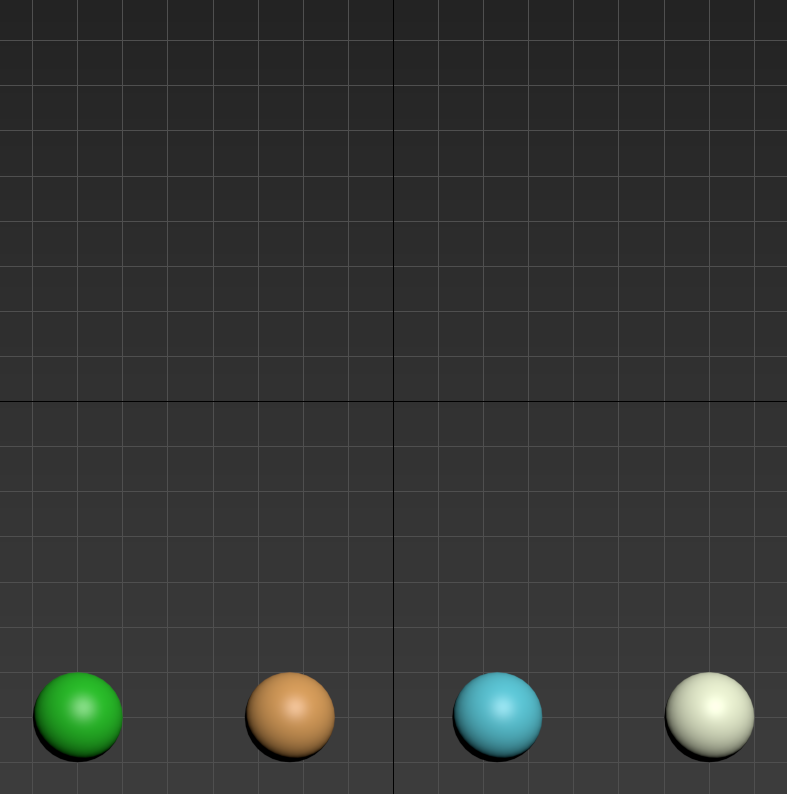
\includegraphics[width=\textwidth]{imagenes/Ejercicio 1/keyframes/0.png}
        \caption{Pelotas en el instante 0.}
    \end{subfigure}
    \hfill
    \begin{subfigure}[H]{0.48\textwidth}
        \centering
        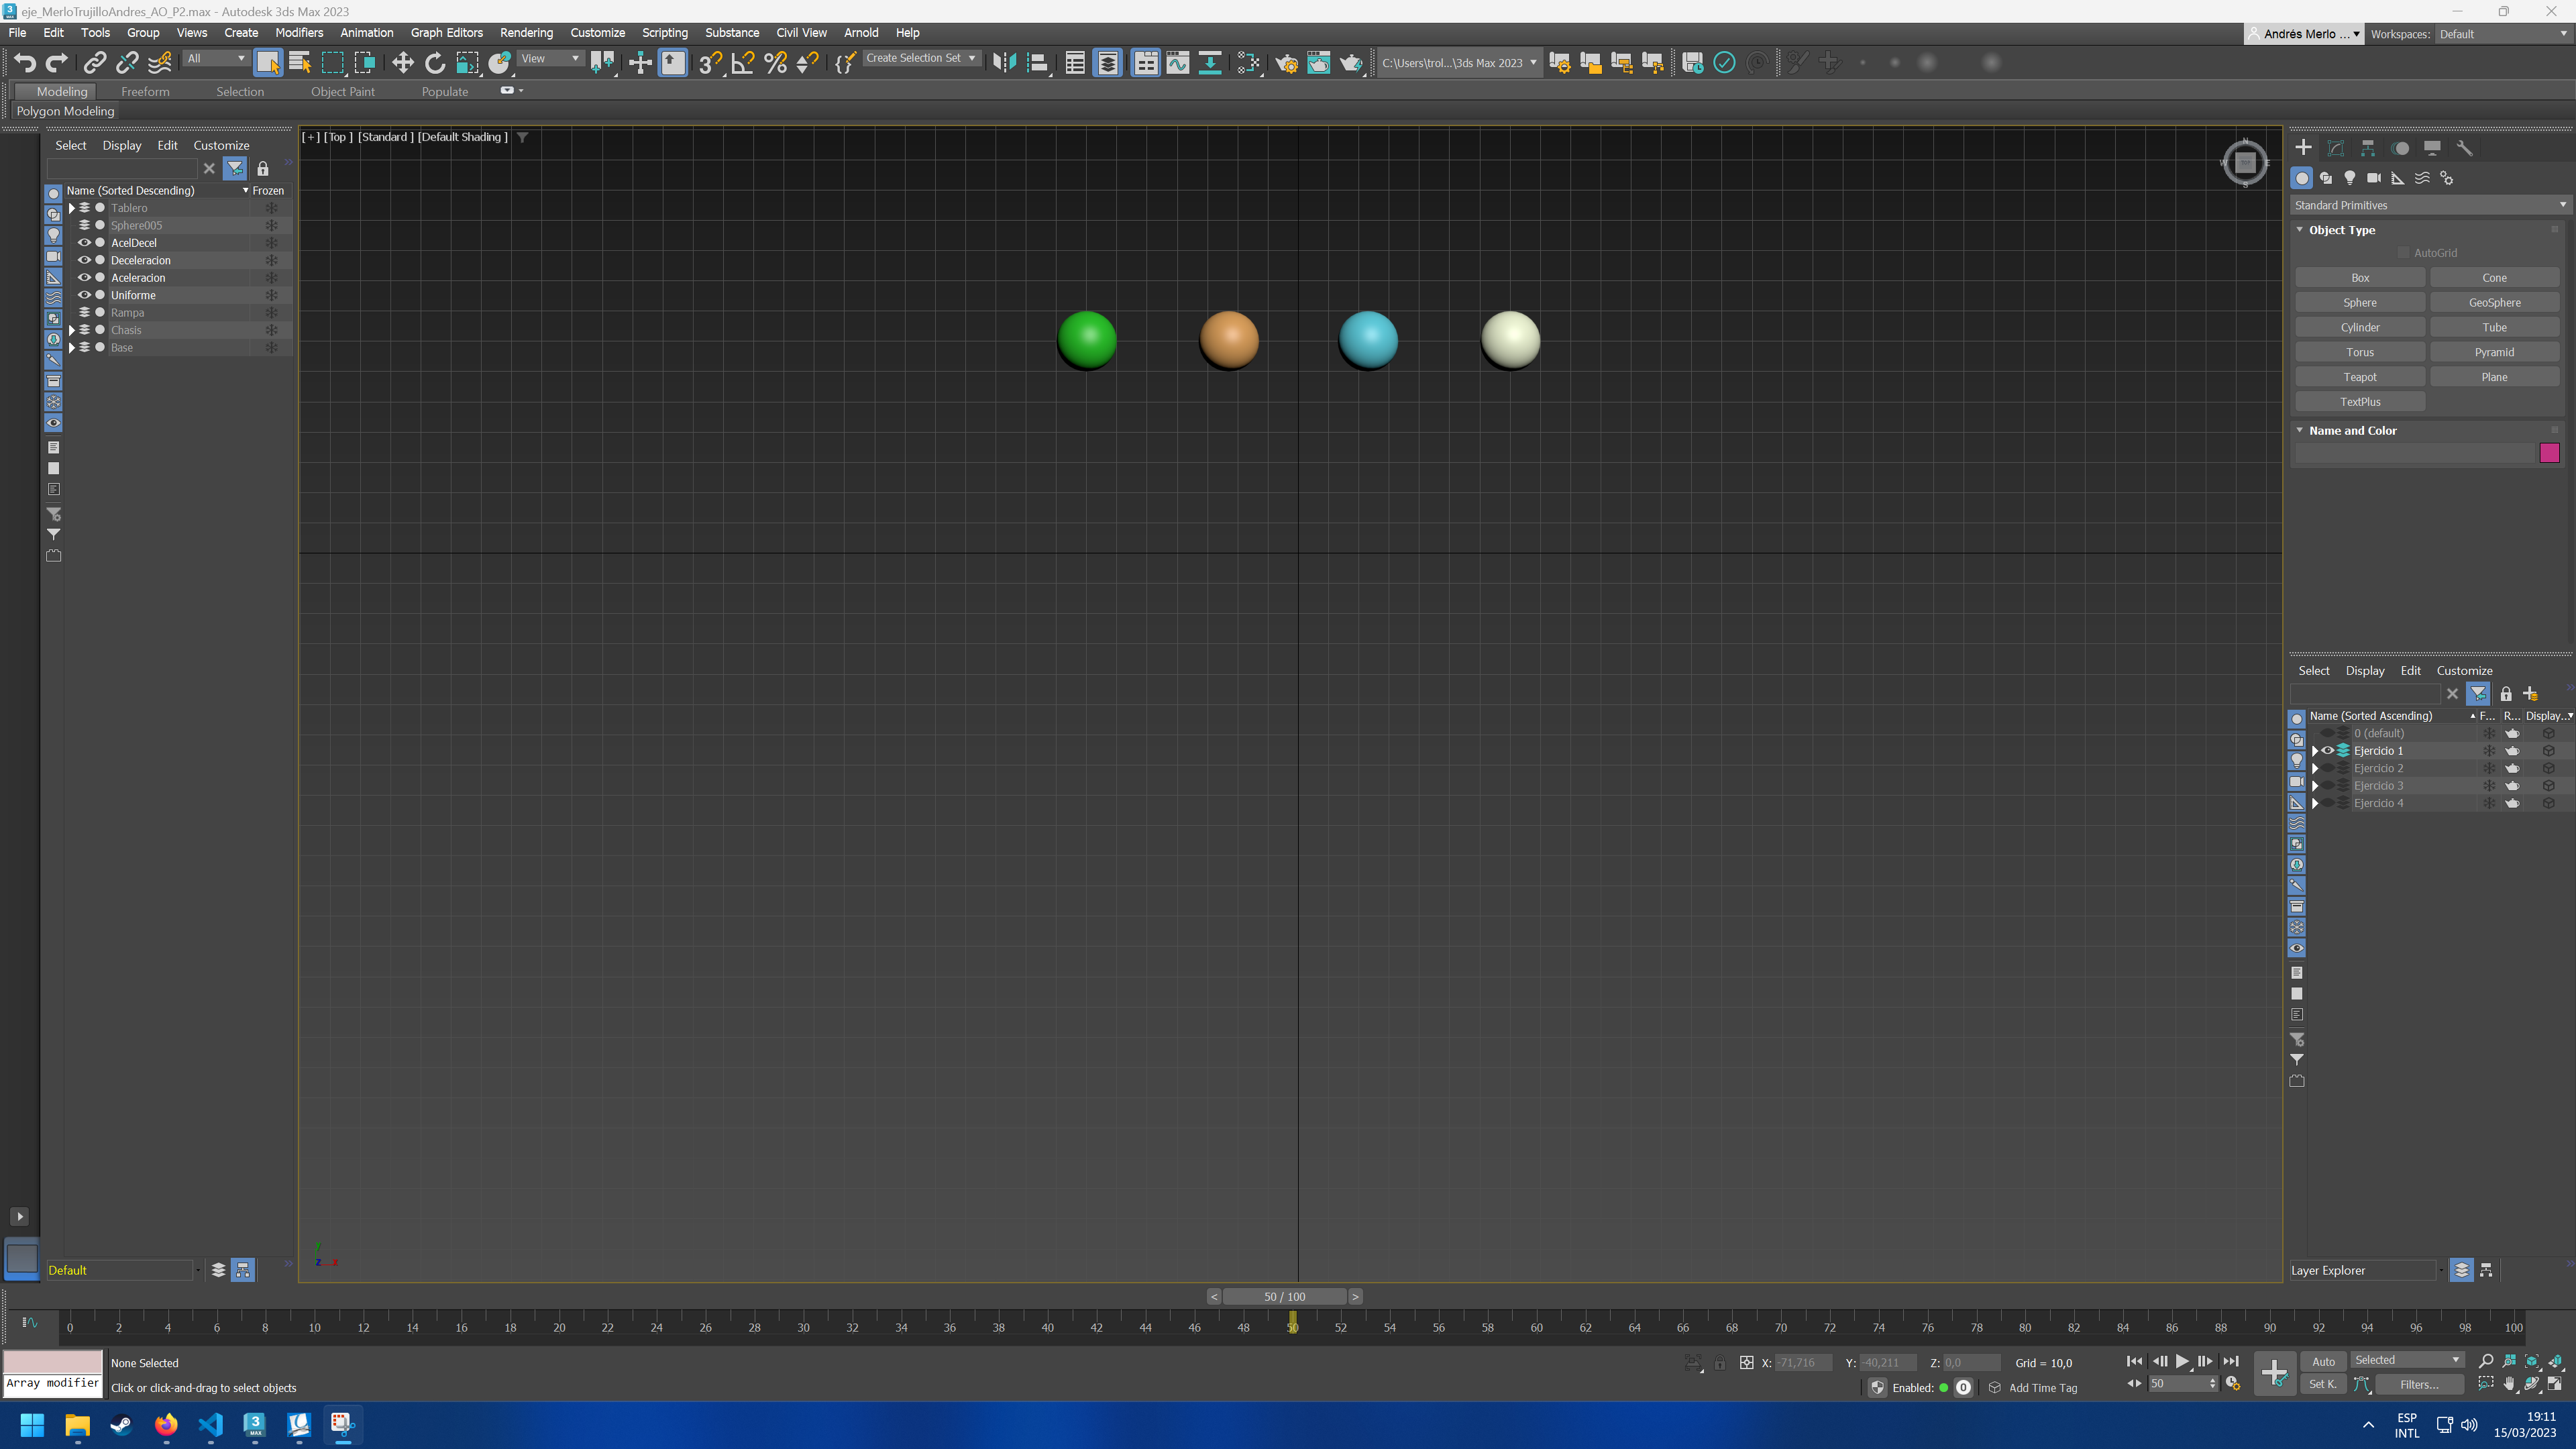
\includegraphics[width=\textwidth]{imagenes/Ejercicio 1/keyframes/50.png}
        \caption{Pelotas en el instante 50.}
    \end{subfigure}
\end{figure}

Estas animaciones las voy a dividir en subsecciones para explicar mejor como son las curvas.

\newpage

\subsection{Movimiento uniforme}

Para esta animación es necesario utilizar una curva lineal, que permita avanzar siempre la misma distancia en cada instante de tiempo. La función tiene la siguiente forma:

%foto de la curva
\begin{figure}[H]
    \centering
    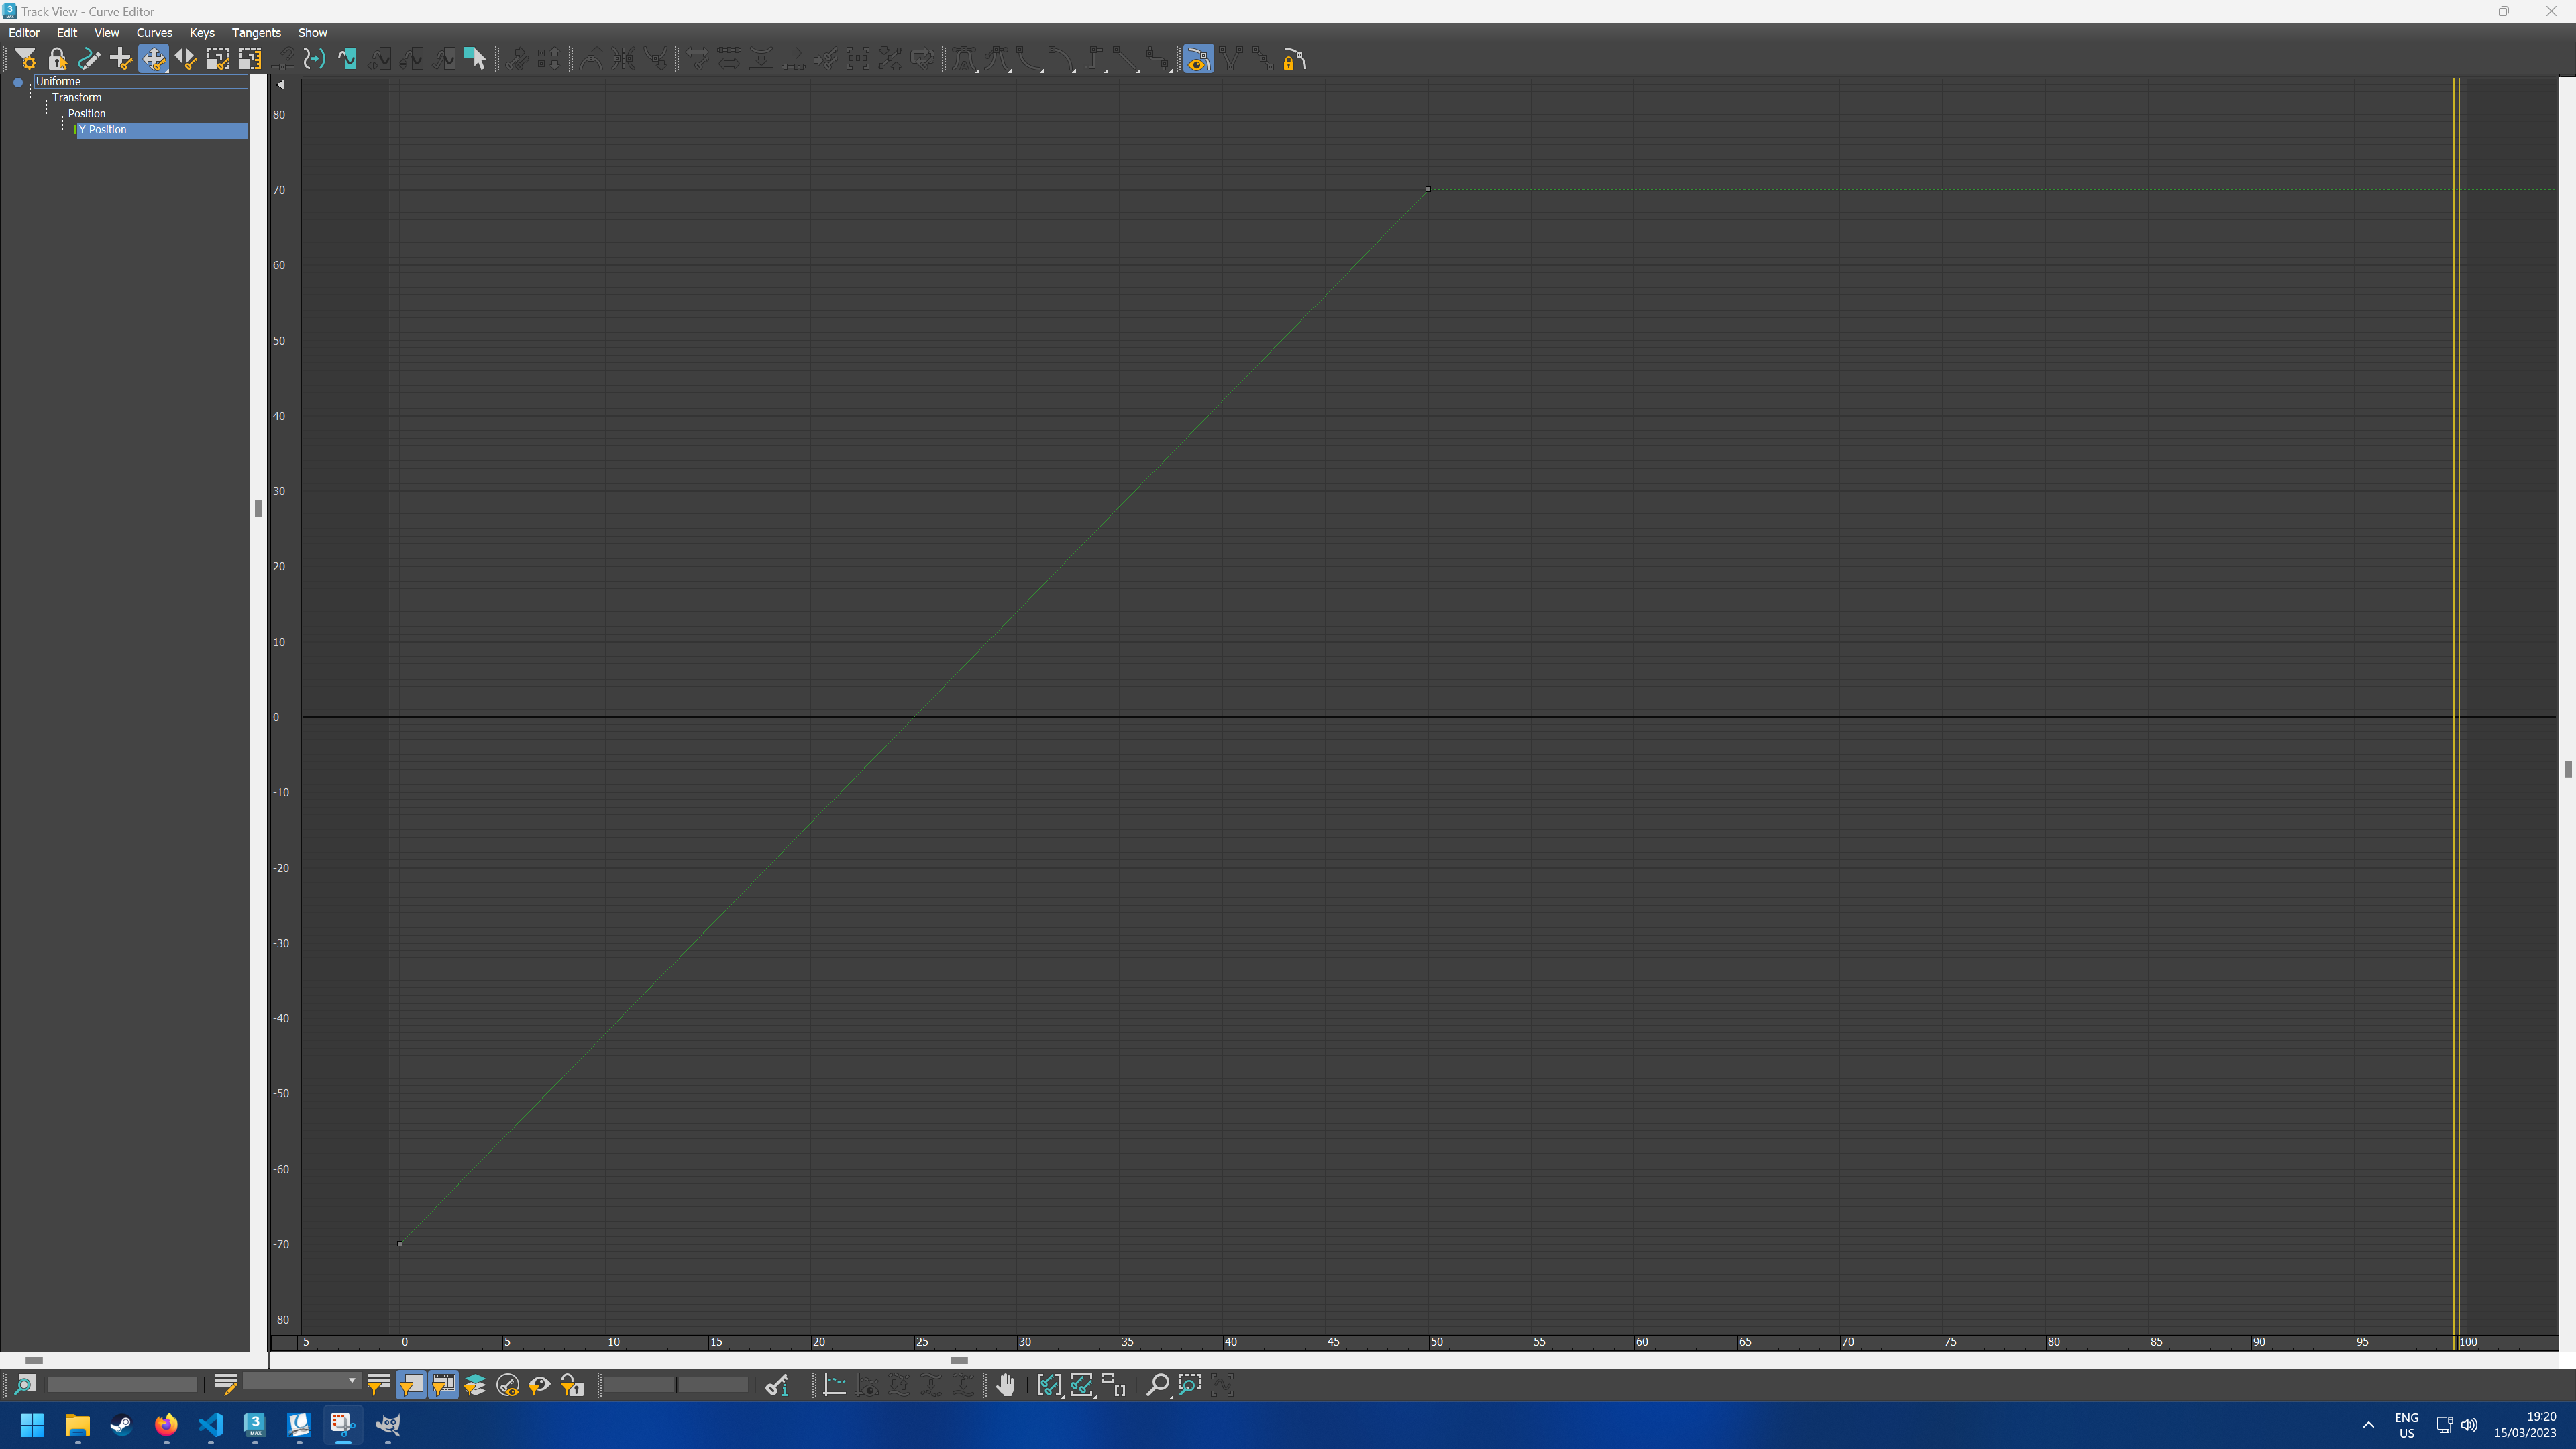
\includegraphics[width=0.6\textwidth]{imagenes/Ejercicio 1/curvas/uniforme.png}
    \caption{Curva de la pelota con movimiento uniforme.}
\end{figure}

En la animación se puede apreciar cómo la pelota mantiene su velocidad constante desde la posición inicial hasta la final.

\newpage

\subsection{Aceleración}

Para realizar esta animación se debe usar una curva de aceleración cuya pendiente sea creciente. Esto hará que la pelota recorra progresivamente una mayor distancia en la misma cantidad de tiempo.

\bigskip

La curva tiene la siguiente forma:

%foto de la grafica
\begin{figure}[H]
    \centering
    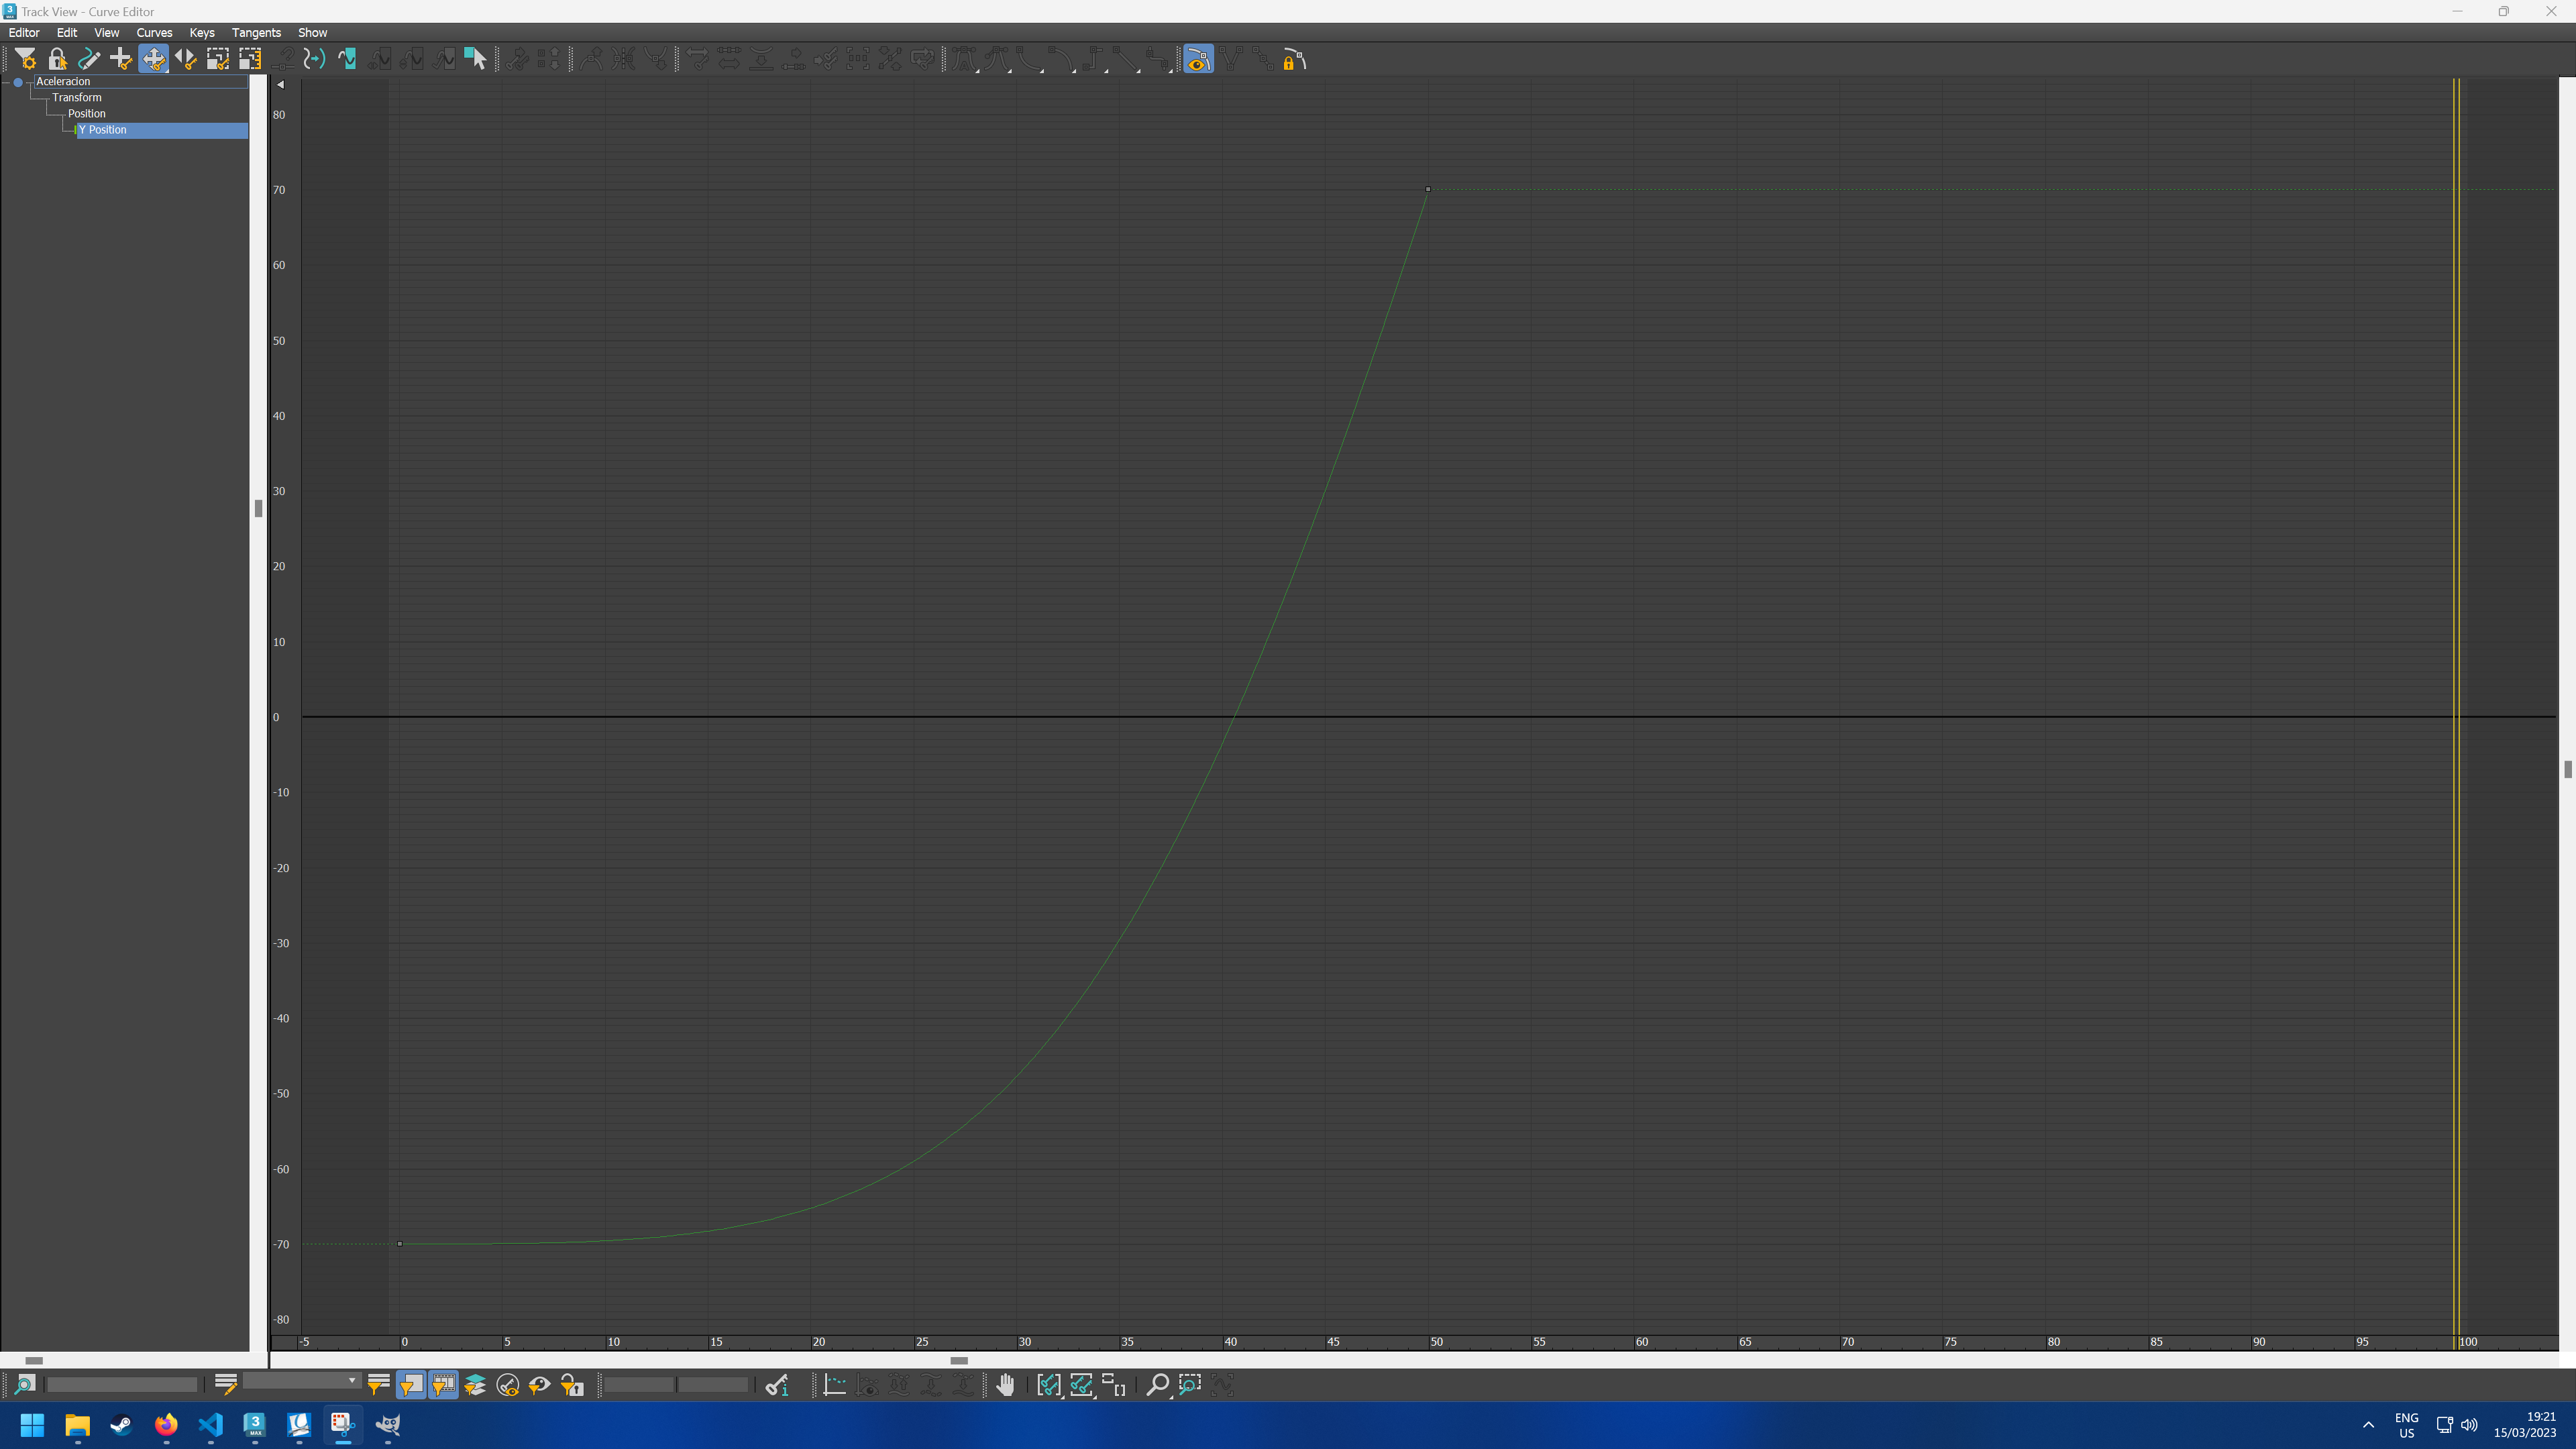
\includegraphics[width=0.6\textwidth]{imagenes/Ejercicio 1/curvas/aceleracion.png}
    \caption{Curva de la pelota que acelera.}
\end{figure}

En la animación se puede observar como la pelota acelera gradualmente hasta que se detiene abruptamente en el punto B.

\bigskip

Cabe decir que he modificado la forma de la curva para que se pueda apreciar con mayor claridad la aceleración en la animación, dado que la curva por defecto del programa no es lo suficientemente pronunciada como para apreciarlo.

\newpage

\subsection{Deceleración}

En este caso, se debe utilizar una curva de desaceleración, similar a la curva de aceleración, pero con una pendiente cada vez menor. Esto provocará que la pelota recorra una distancia cada vez menor en la misma cantidad de tiempo, logrando así que finalmente se detenga en el punto B.

\bigskip

La curva tiene la siguiente forma:

%foto de la curva
\begin{figure}[H]
    \centering
    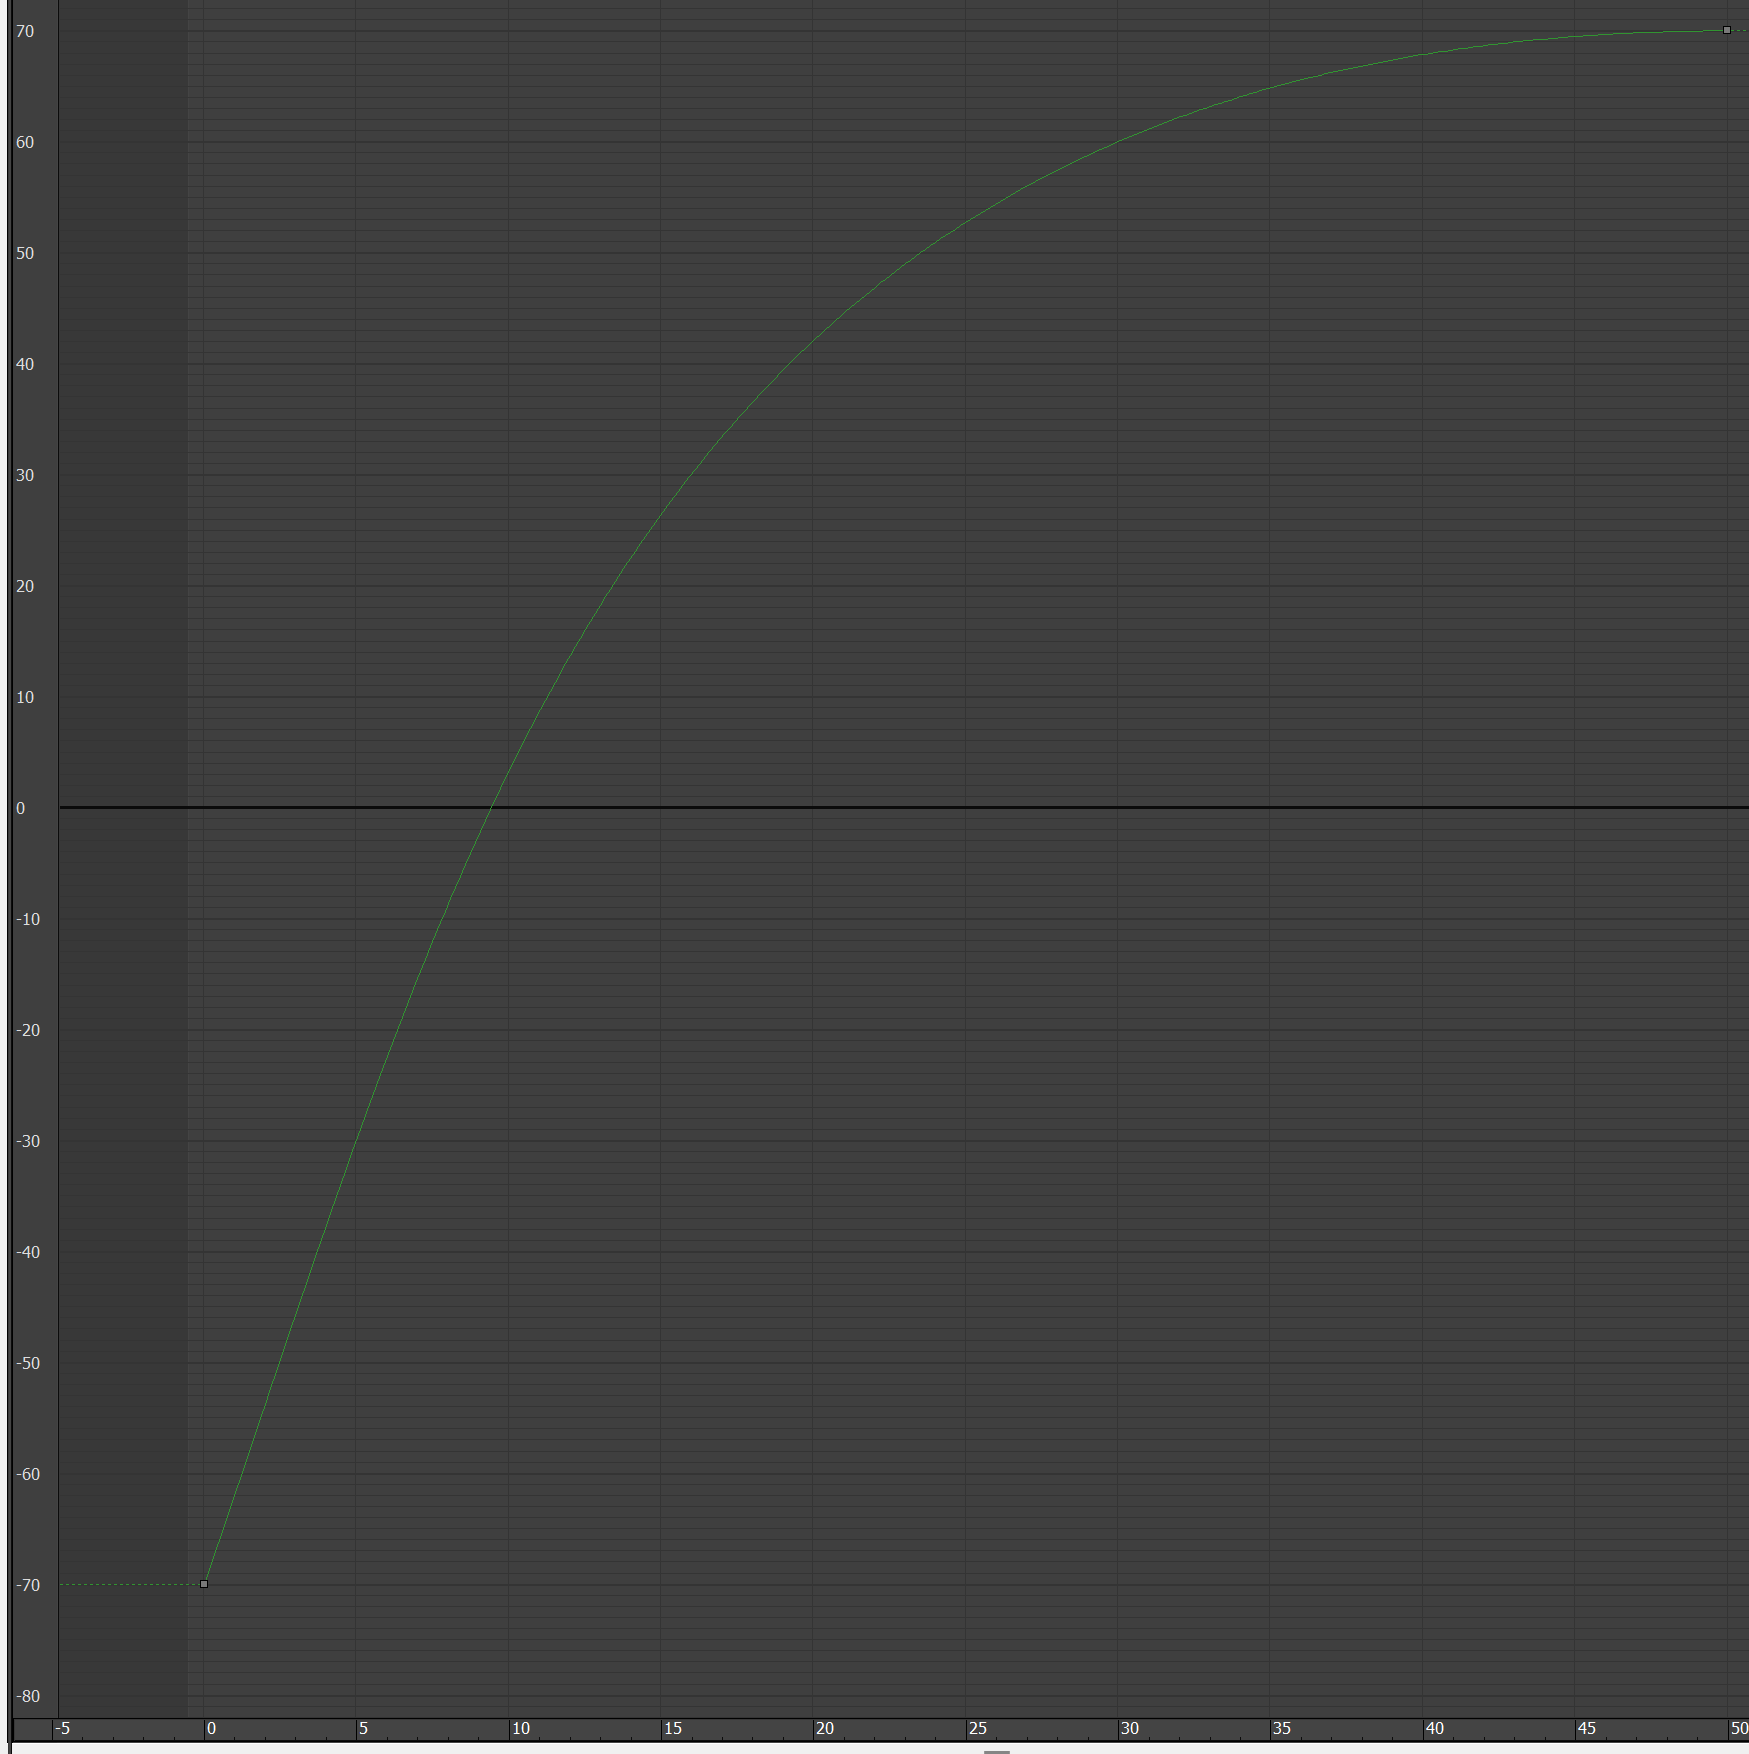
\includegraphics[width=0.6\textwidth]{imagenes/Ejercicio 1/curvas/deceleracion.png}
    \caption{Curva de la pelota que desacelera.}
\end{figure}

En la animación, la pelota comienza moviéndose a gran velocidad y a medida que se acerca a su posición final, disminuye su velocidad hasta detenerse por completo.

\bigskip

Al igual que con la aceleración, he modificado la curva para que el frenado sea más pronunciado.

\newpage

\subsection{Aceleración y deceleración}

Esta animación es el resultado de combinar las versiones de aceleración y deceleración, lo que provoca que la pelota acelere al salir del punto A y desacelere al acercarse al punto B.

\bigskip

La curva resultante es la unión de ambas versiones, con una pendiente que aumenta progresivamente hasta alcanzar un punto en el que comienza a disminuir.

Dicha curva es la siguiente:

%imagen de la curva
\begin{figure}[H]
    \centering
    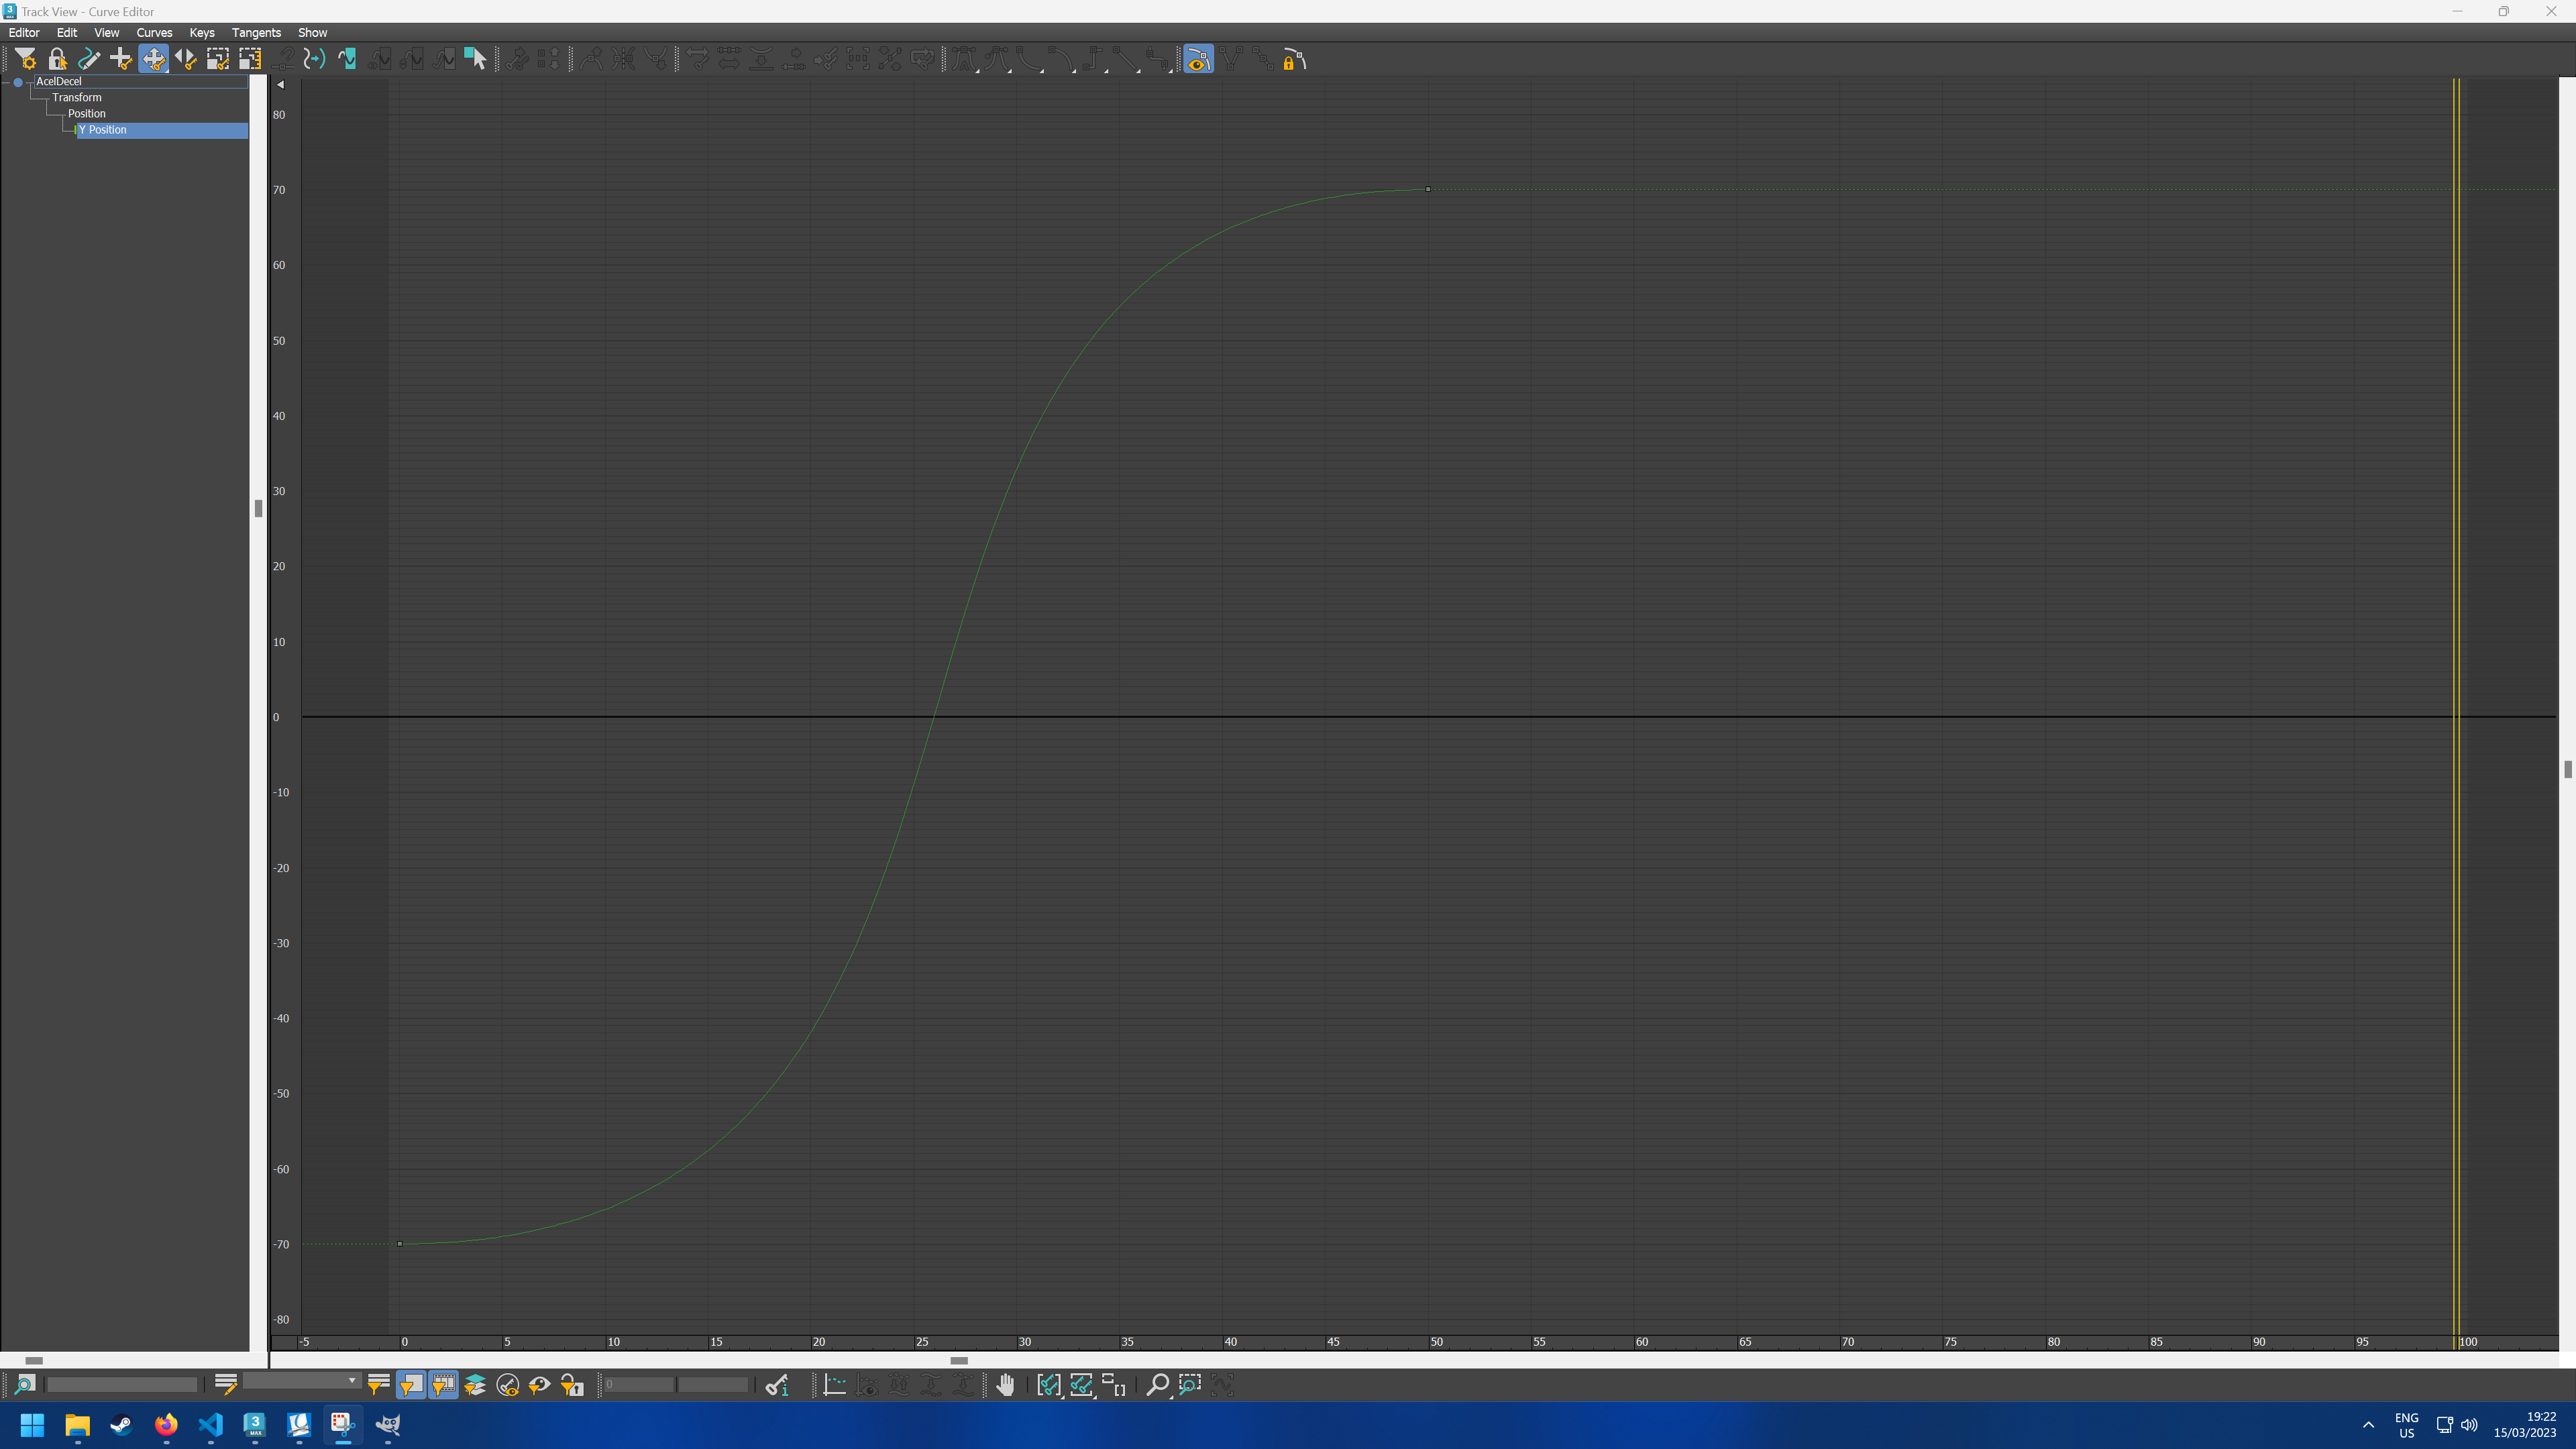
\includegraphics[width=0.6\textwidth]{imagenes/Ejercicio 1/curvas/aceldecel.png}
    \caption{Curva de la pelota que acelera y desacelera.}
\end{figure}

Como resultado, la pelota acelera al principio y comienza a desacelerar al acercarse al punto final. Además, al igual que en las subsecciones anteriores, he modificado la curva para que el resultado sea más fácil de apreciar.

\newpage

\section{Ejercicio 2 - Salto de coche}

En este ejercicio se pide animar un coche que parte desde una posición inicial, sube una rampa, la salta y finalmente frena al tocar el suelo.

% no se si poner como he hecho la rampa.
\bigskip

%reescribir esto
Cabe destacar que para animar la rotación necesaria para subir a la rampa, he cambiado el pivote del coche para que se sitúe justo en el eje de las ruedas traseras, ya que esto representa mejor el movimiento real al subir dicha rampa.

\bigskip

Además, para la jerarquía de objetos, he utilizado el cubo más grande del vehículo como padre y las ruedas y el cubo más pequeño como hijos.

\bigskip

La animación consiste en 8 \textit{keyframes}, que son los siguientes:

\begin{enumerate}
    \item \textbf{Instante 0:} El vehículo se encuentra en la posición inicial y está listo para acelerar.
    \item \textbf{Instante 19:} El vehículo ha acelerado.
    \item \textbf{Instante 32:} El vehículo se encuentra en el instante anterior de subir la rampa.
    \item \textbf{Instante 34:} El vehículo ha subido la rampa y se encuentra al principio de la misma.
    \item \textbf{Instante 39:} El vehículo se encuentra en el instante anterior de estar en el aire; es decir, se encuentra tocando el final de la rampa solo con la rueda trasera.
    \item \textbf{Instante 50:} El vehículo se encuentra en el punto más alto del lanzamiento y ya recto (paralelo al suelo).
    \item \textbf{Instante 62:} El vehículo ha tocado el suelo después del salto y va a comenzar a frenar.
    \item \textbf{Instante 86:} El vehículo ha frenado y se encuentra parado.
\end{enumerate}

\bigskip

A modo visual, los \textit{keyframes} son los siguientes:

%fotos de los keyframes

\begin{figure}[H]
    \centering
    \begin{subfigure}[H]{0.48\textwidth}
        \centering
        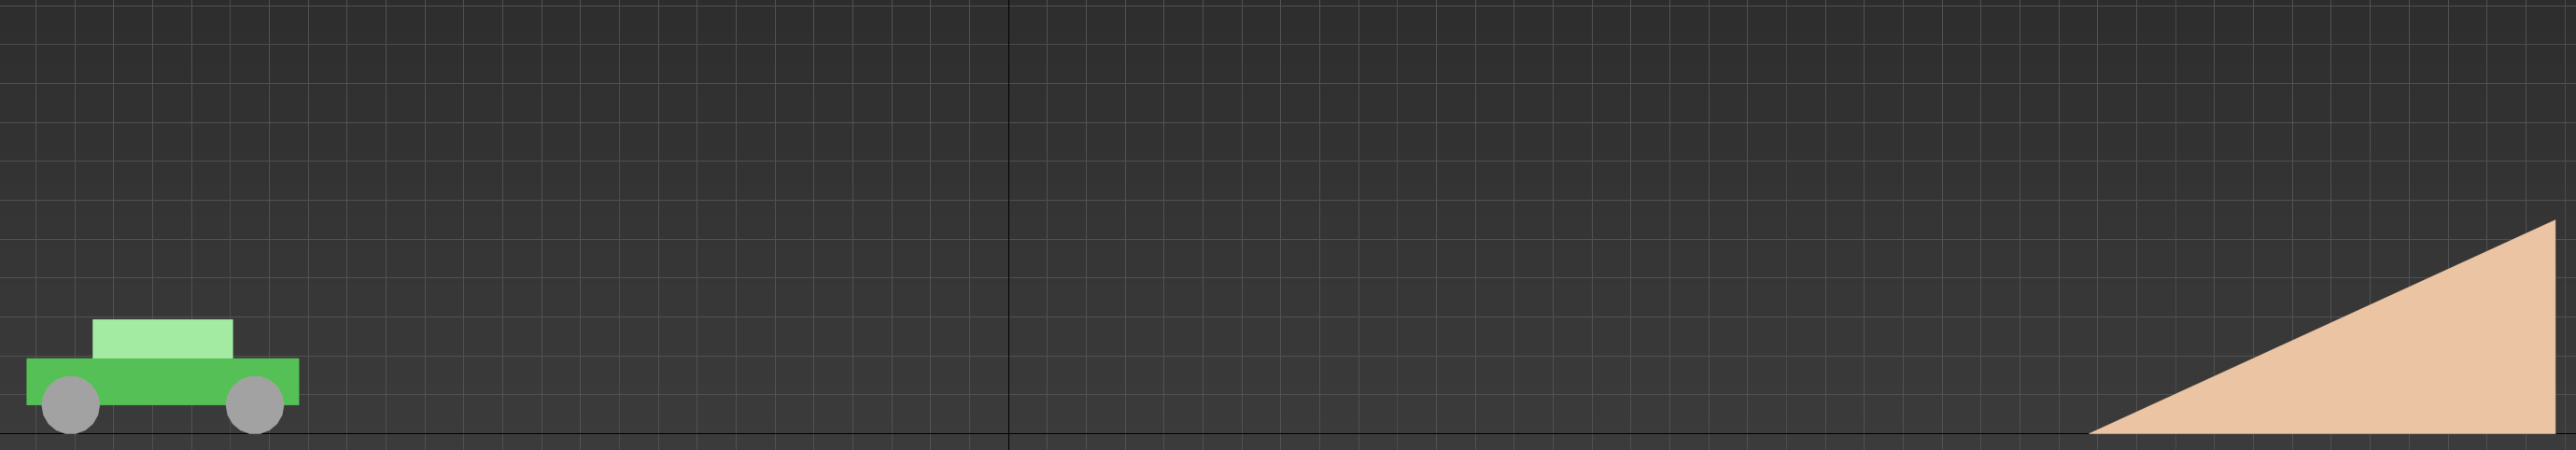
\includegraphics[width=\textwidth]{imagenes/Ejercicio2/corregidas/keyframes/0.png}
        \caption{Vehículo en el instante 0.}
    \end{subfigure}
    \hfill
    \begin{subfigure}[H]{0.48\textwidth}
        \centering
        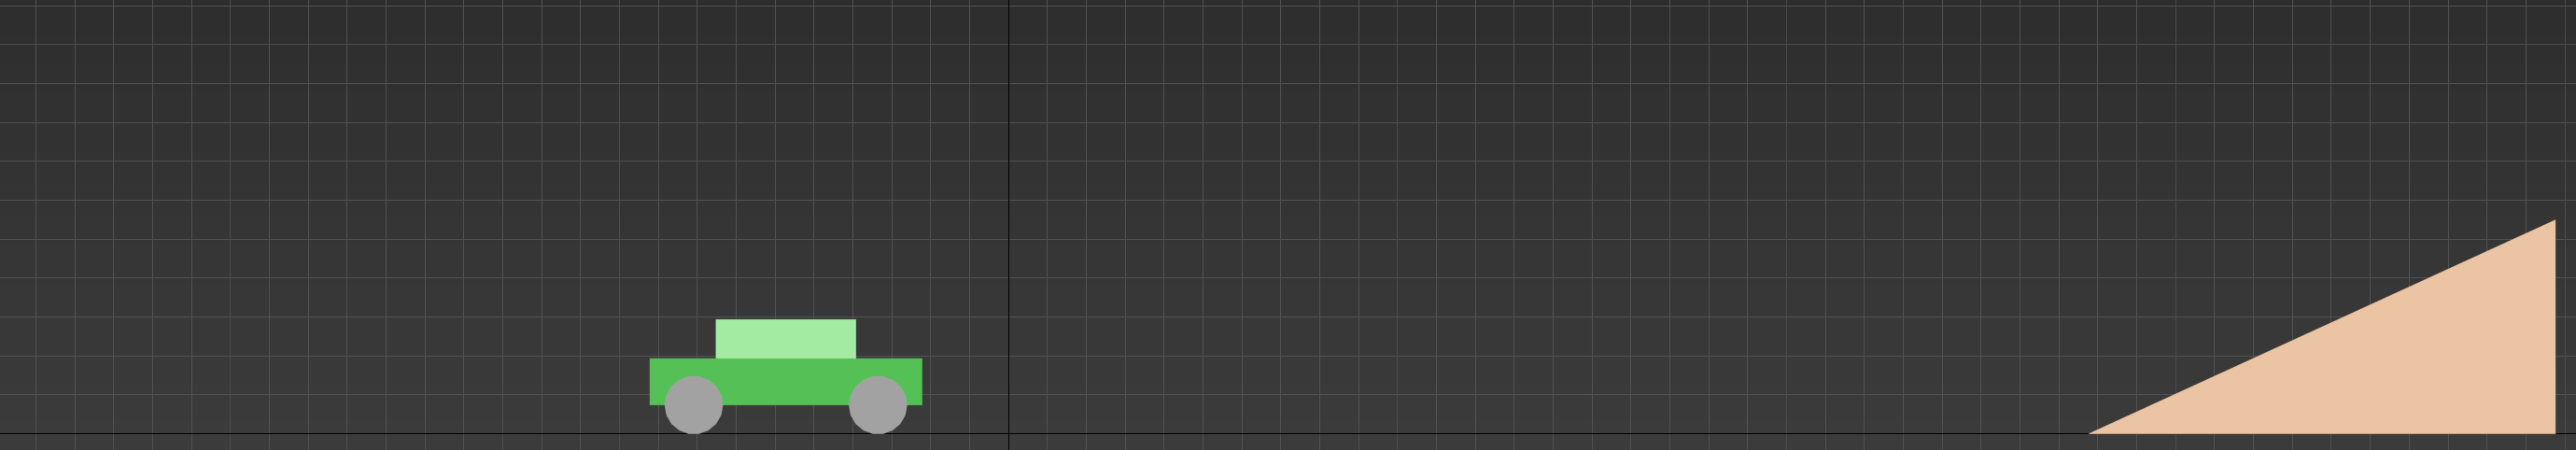
\includegraphics[width=\textwidth]{imagenes/Ejercicio2/corregidas/keyframes/19.png}
        \caption{Vehículo en el instante 19.}
    \end{subfigure}
    % \hfill
    \par\bigskip
    \begin{subfigure}[H]{0.48\textwidth}
        \centering
        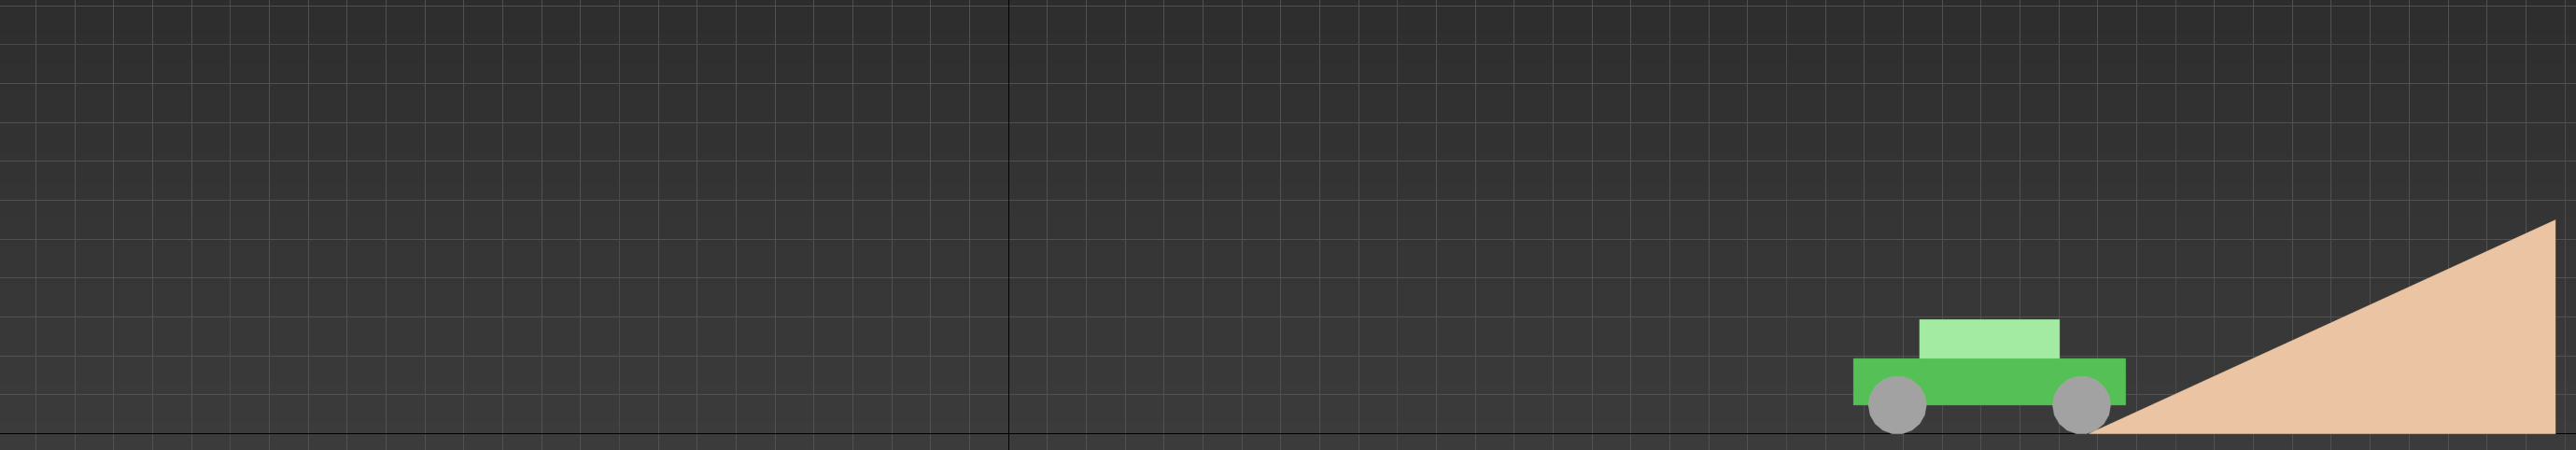
\includegraphics[width=\textwidth]{imagenes/Ejercicio2/corregidas/keyframes/32.png}
        \caption{Vehículo en el instante 32.}
    \end{subfigure}
    \hfill
    \begin{subfigure}[H]{0.48\textwidth}
        \centering
        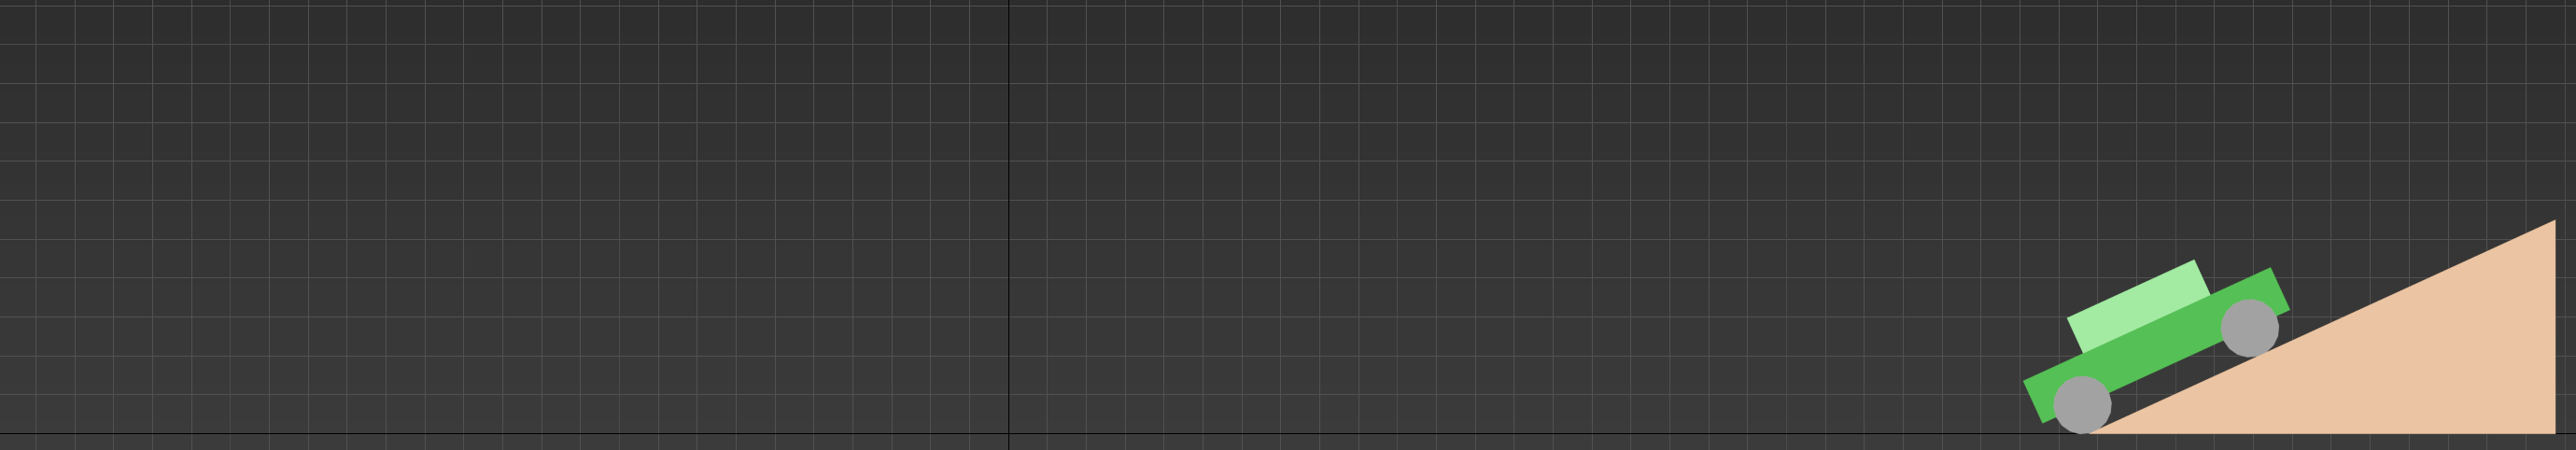
\includegraphics[width=\textwidth]{imagenes/Ejercicio2/corregidas/keyframes/34.png}
        \caption{Vehículo en el instante 34.}
    \end{subfigure}
    % \hfill
    \par\bigskip
    \begin{subfigure}[H]{0.48\textwidth}
        \centering
        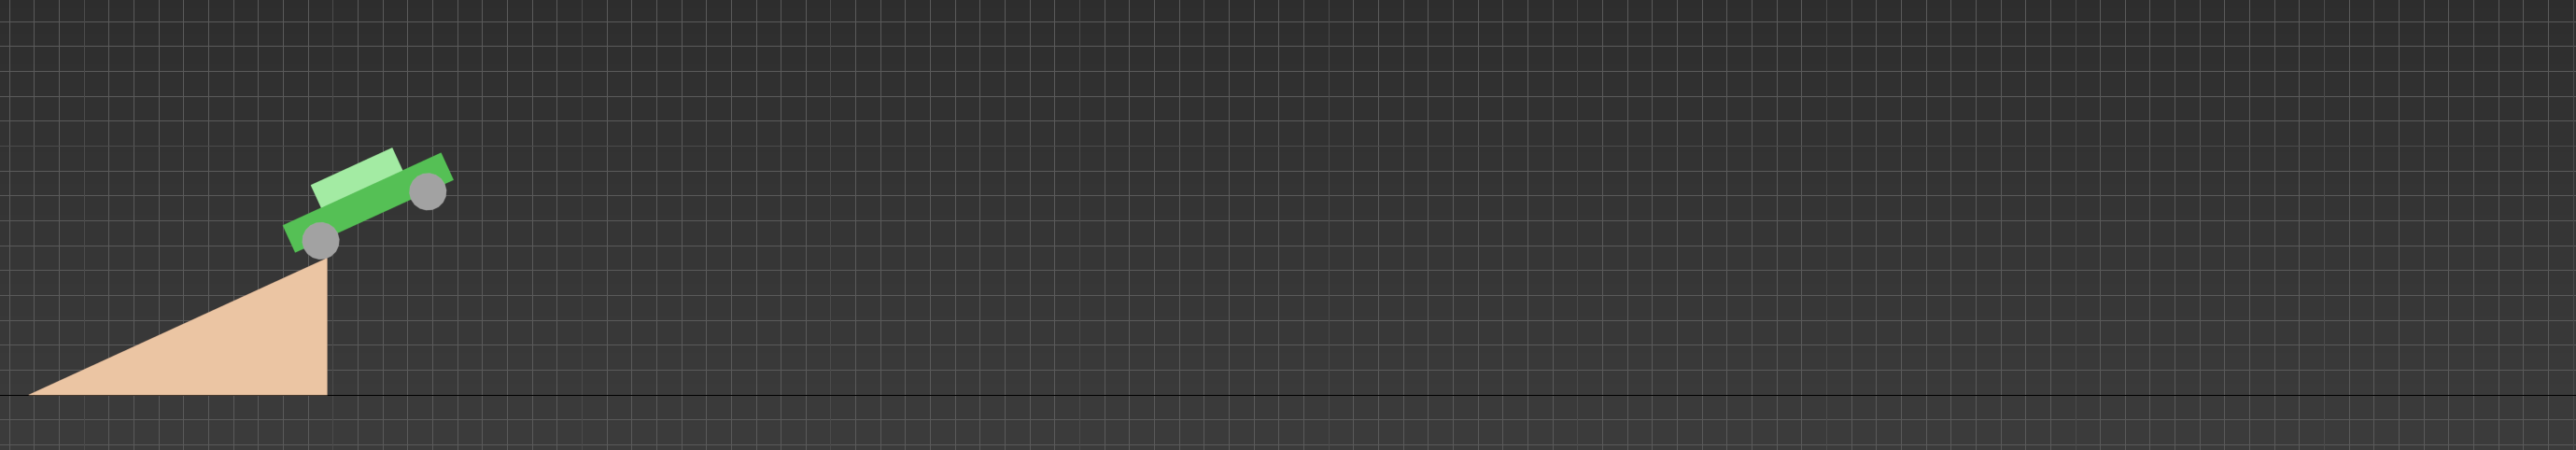
\includegraphics[width=\textwidth]{imagenes/Ejercicio2/corregidas/keyframes/39.png}
        \caption{Vehículo en el instante 39.}
    \end{subfigure}
    \hfill
    \begin{subfigure}[H]{0.48\textwidth}
        \centering
        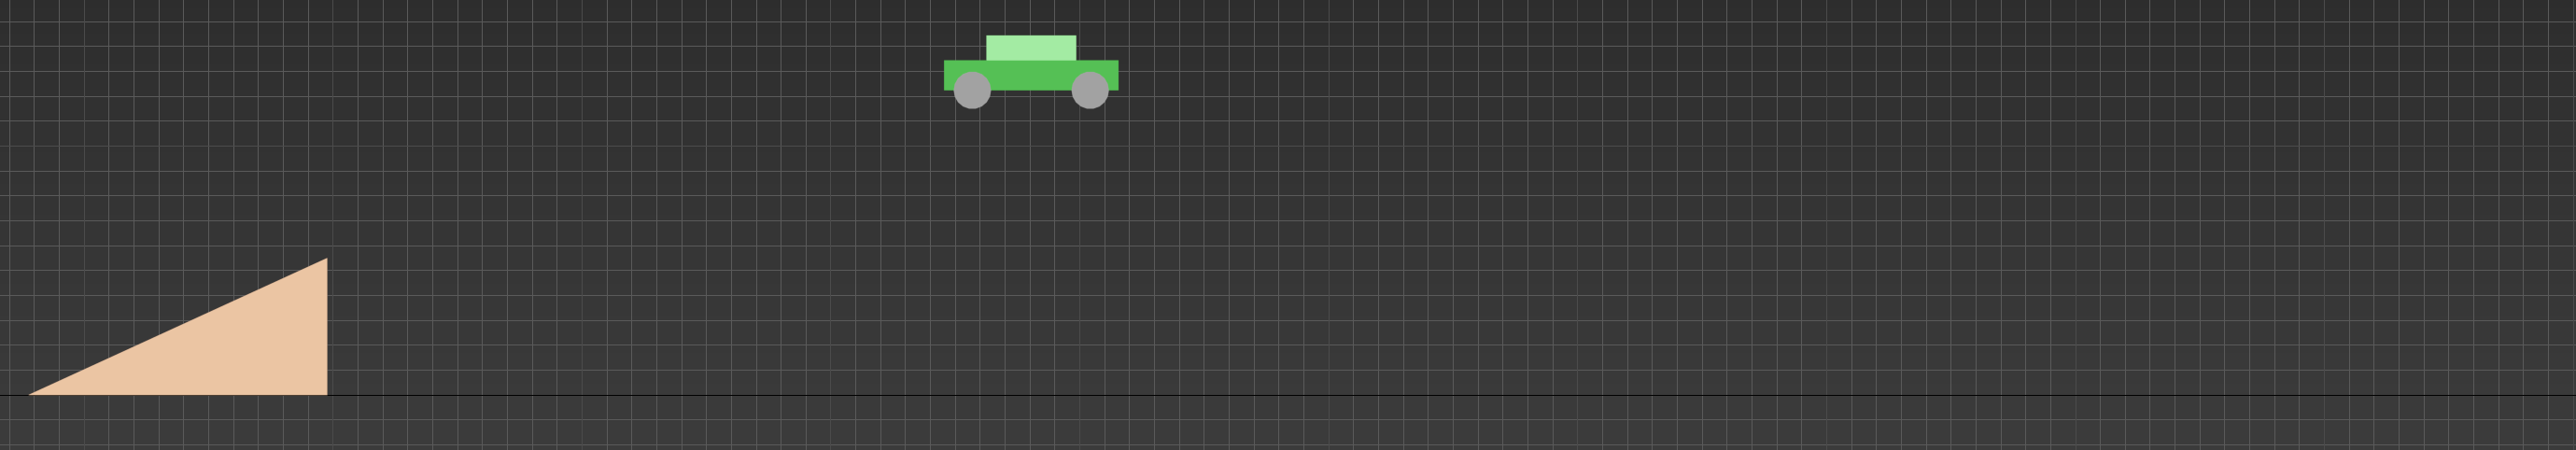
\includegraphics[width=\textwidth]{imagenes/Ejercicio2/corregidas/keyframes/50.png}
        \caption{Vehículo en el instante 50.}
    \end{subfigure}
    % \hfill
    \par\bigskip
    \begin{subfigure}[H]{0.48\textwidth}
        \centering
        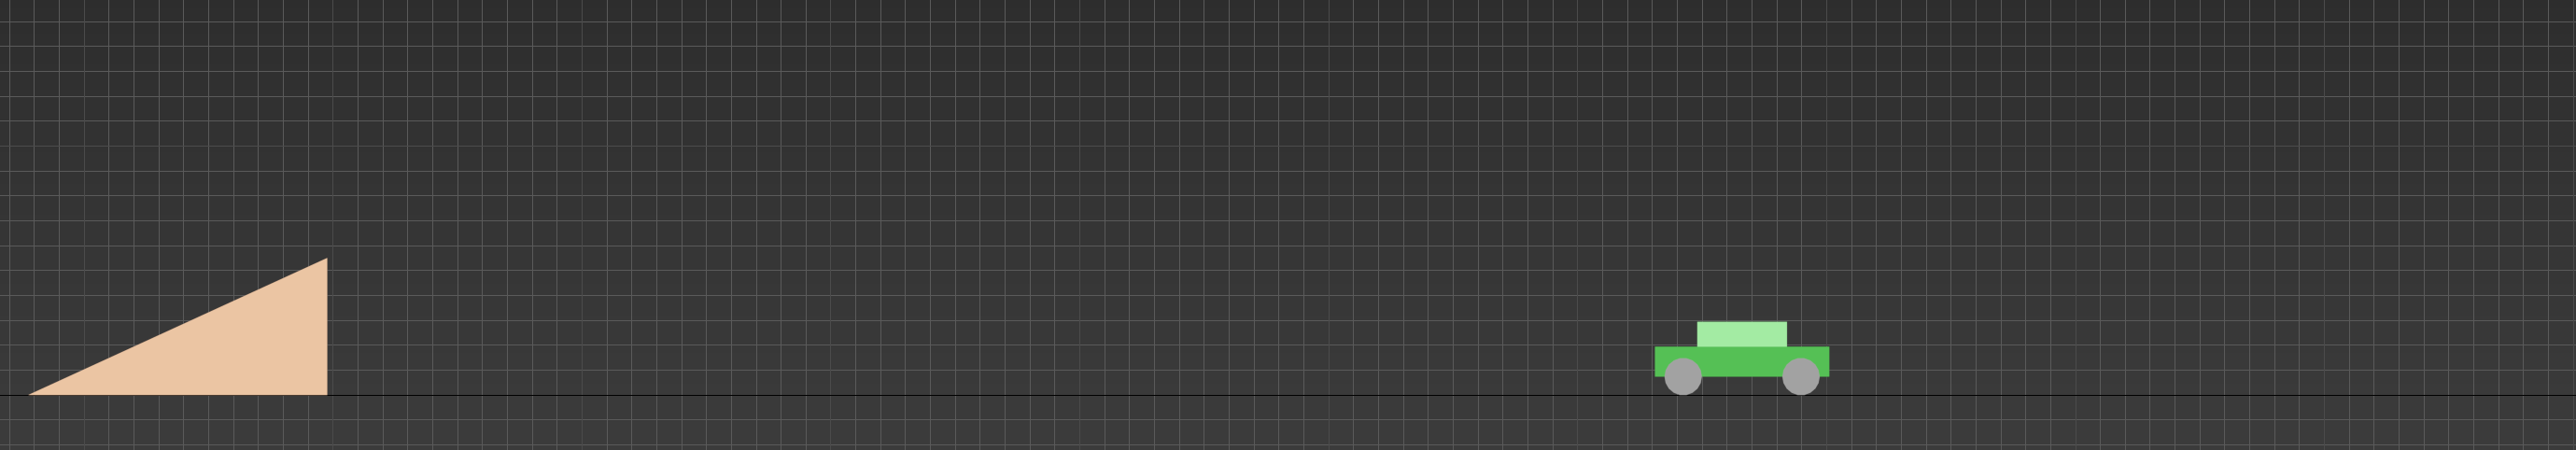
\includegraphics[width=\textwidth]{imagenes/Ejercicio2/corregidas/keyframes/62.png}
        \caption{Vehículo en el instante 62.}
    \end{subfigure}
    \hfill
    \begin{subfigure}[H]{0.48\textwidth}
        \centering
        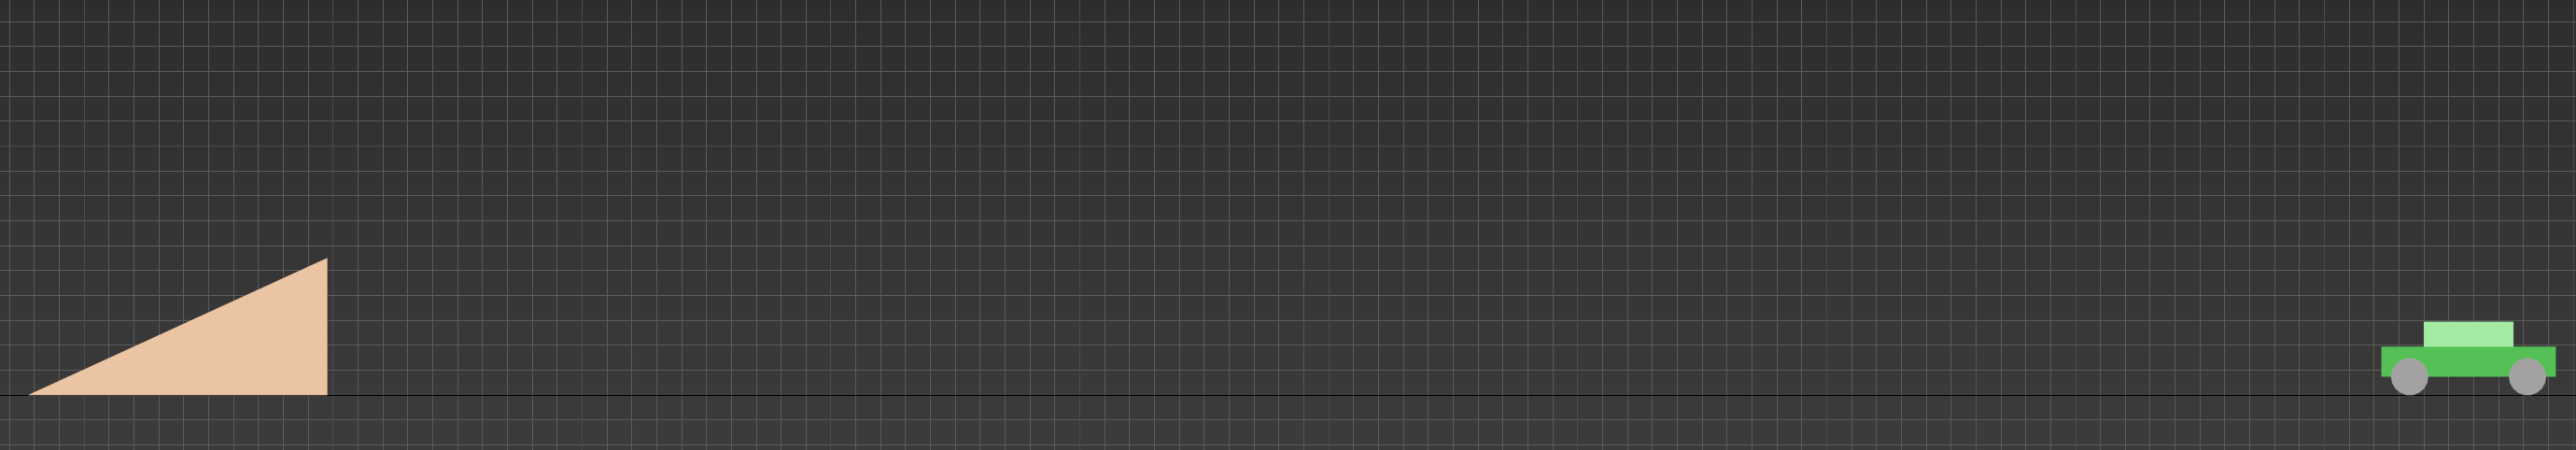
\includegraphics[width=\textwidth]{imagenes/Ejercicio2/corregidas/keyframes/86.png}
        \caption{Vehículo en el instante 86.}
    \end{subfigure}
    \caption{\textit{Keyframes} para animar el coche.}
\end{figure}

\newpage

Y las curvas utilizadas para la animación son:
%fotos de las curvas, separadas por partes (si no son muchas)
\begin{figure}[H]
    \centering
    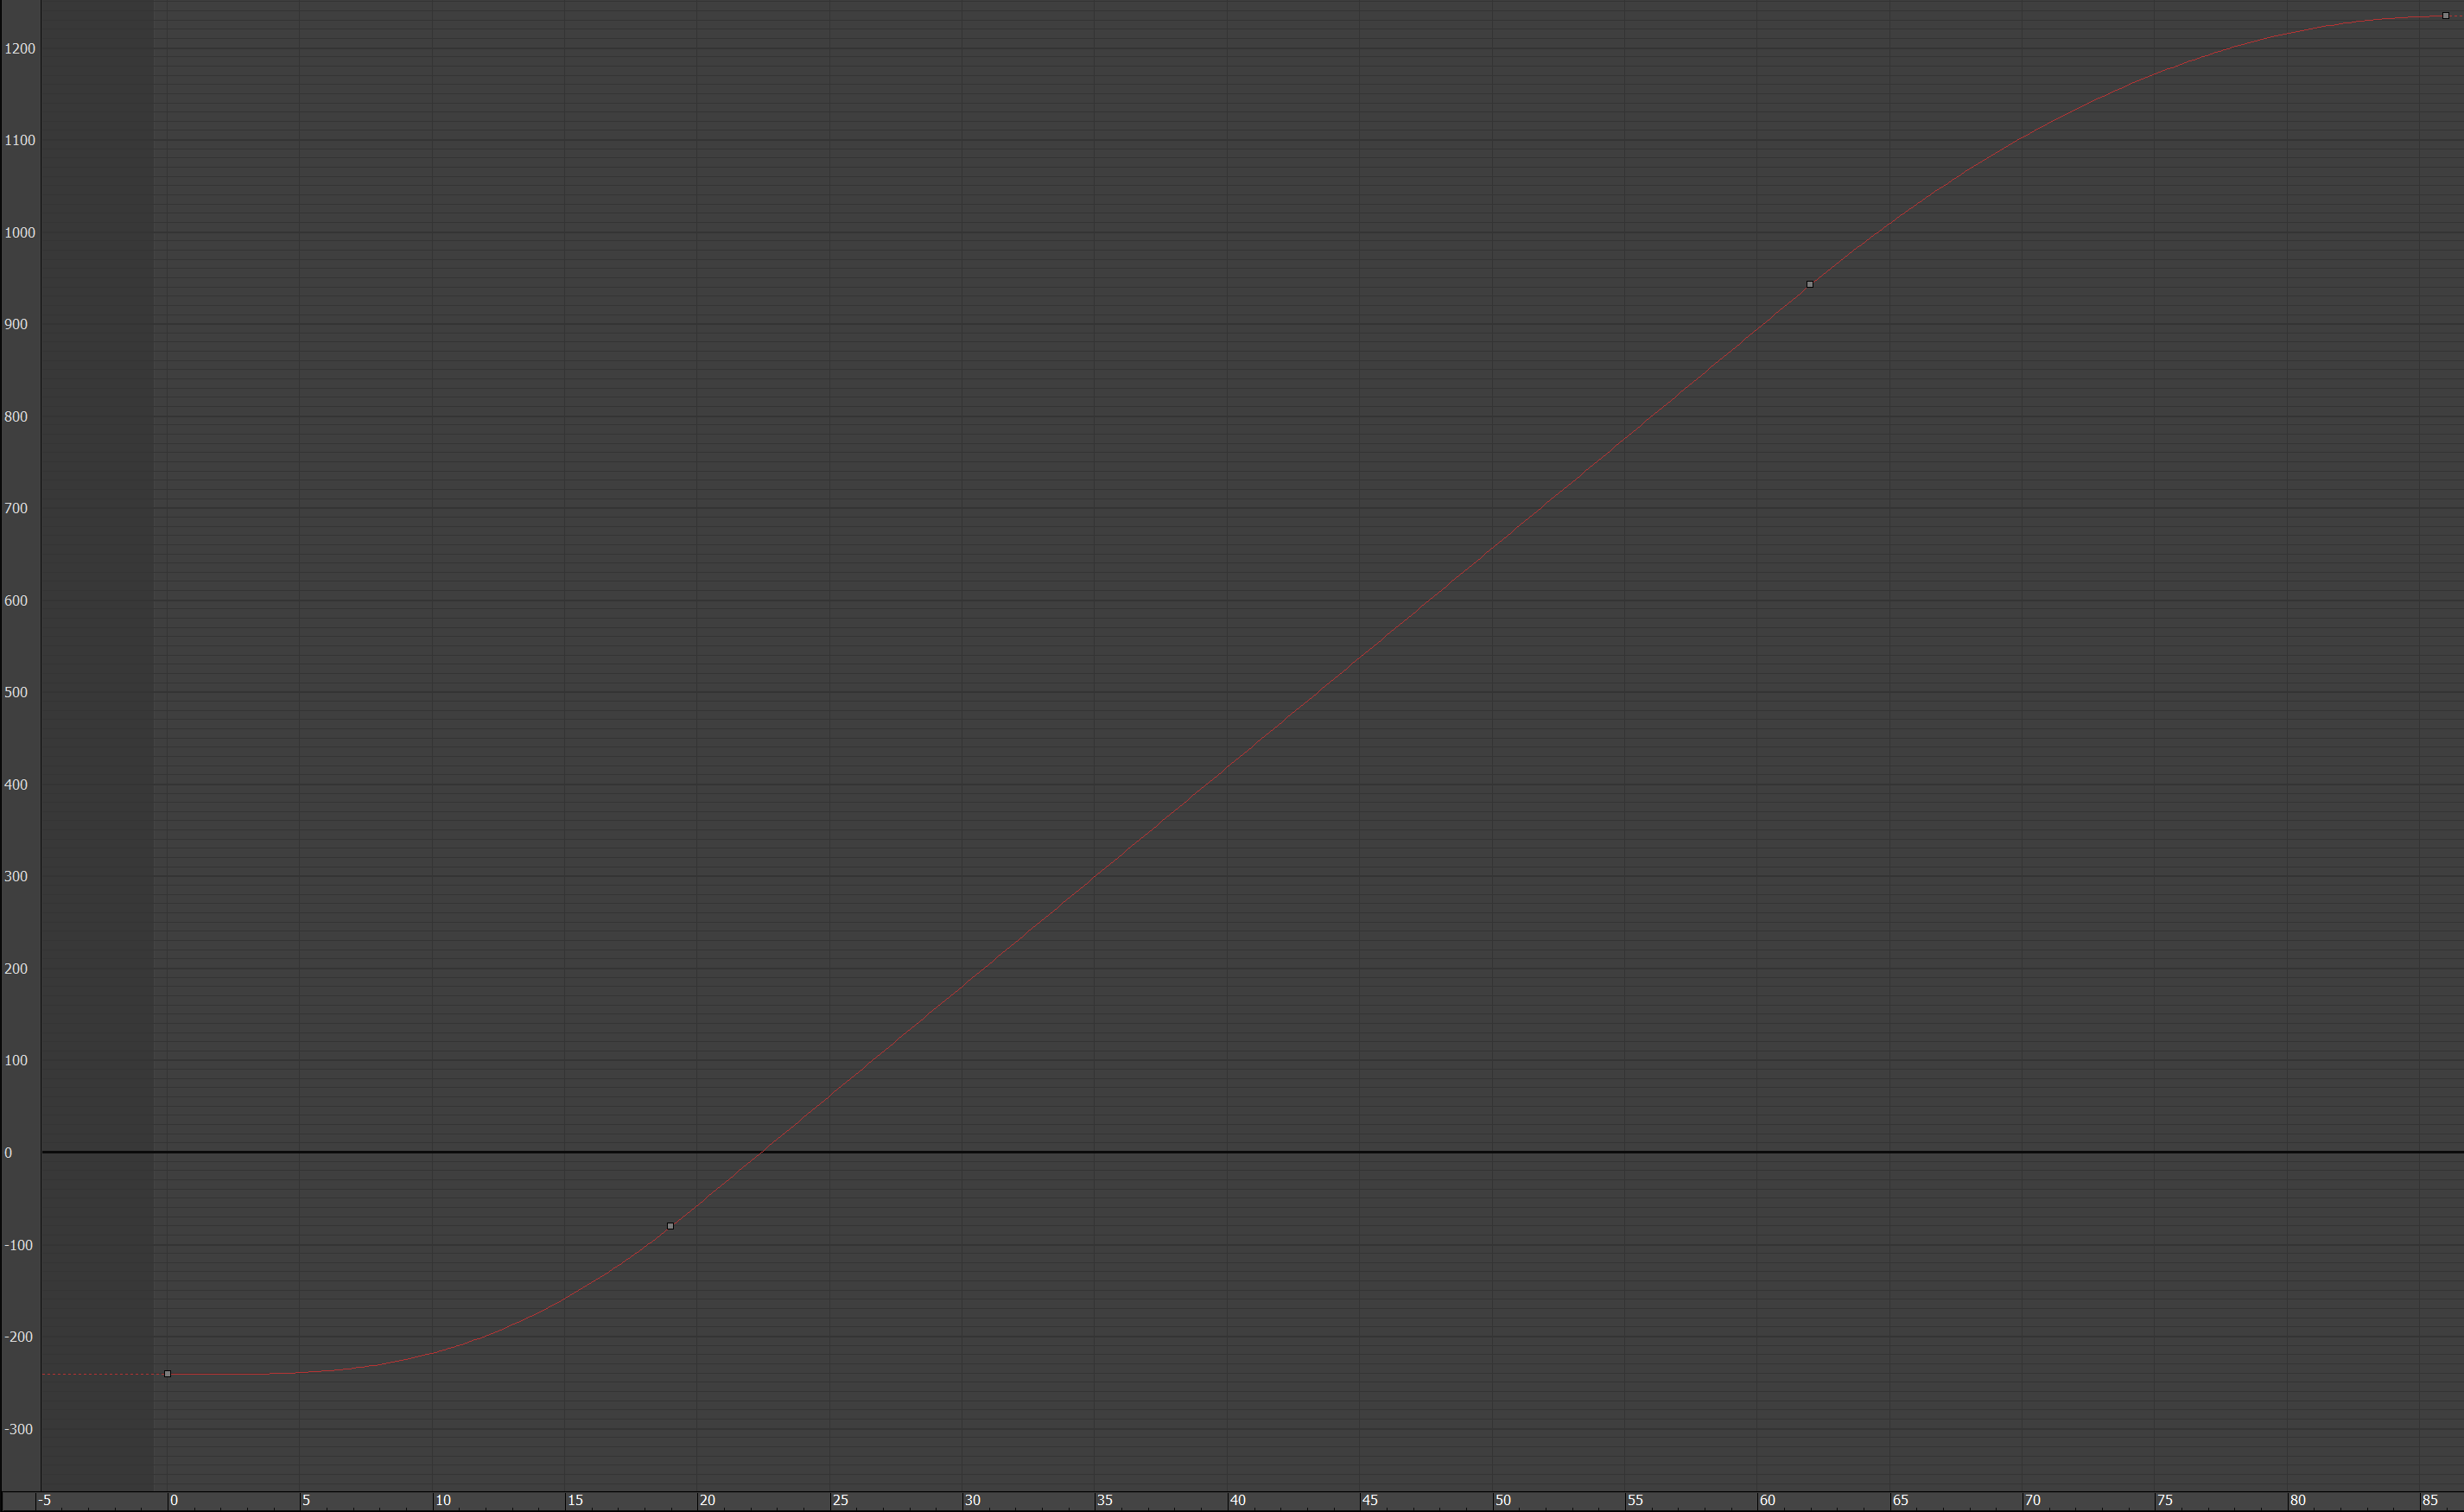
\includegraphics[width=0.8\textwidth]{imagenes/Ejercicio2/corregidas/curvas/red.png}
    \caption{Curva referente a la posición del vehículo en el eje X.}
\end{figure}

Como se puede ver en la curva roja (posición en el eje X), al principio tiene forma exponencial creciente para simular la aceleración, seguida de un tramo lineal hasta la parte de frenado, donde la curva tiene forma exponencial decreciente para que el coche frene y se detenga.

\begin{figure}[H]
    \centering
    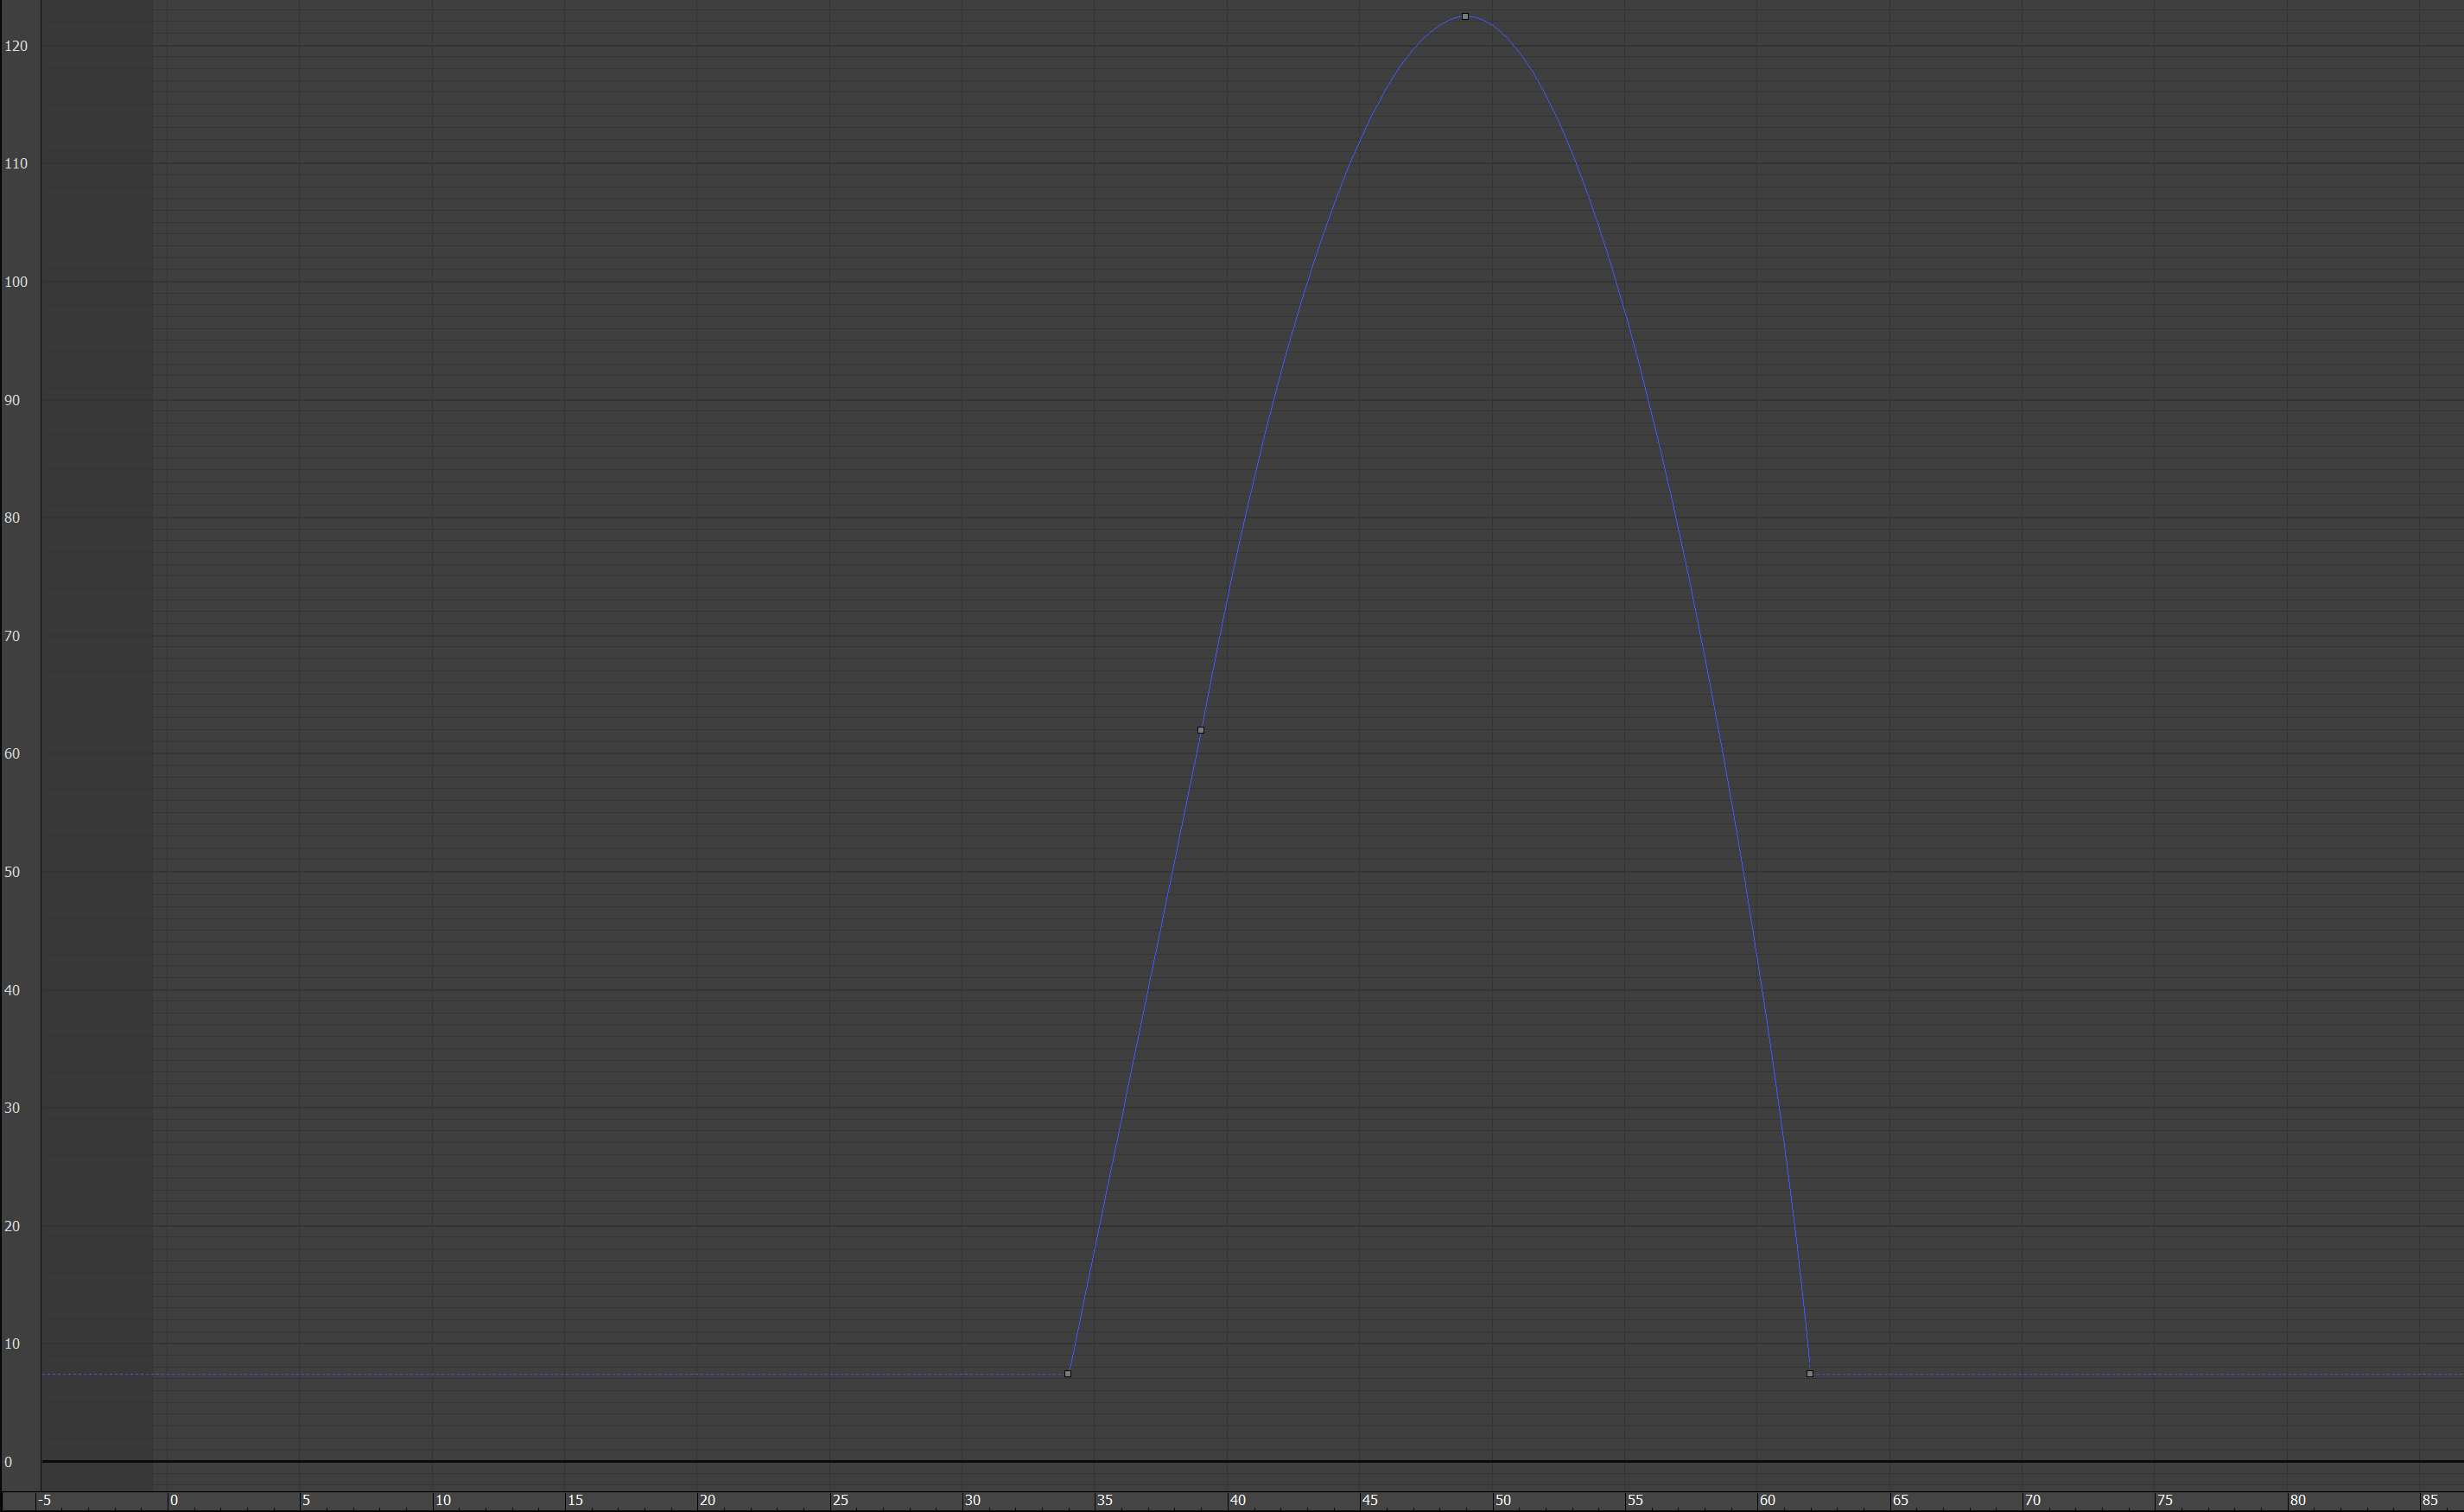
\includegraphics[width=0.8\textwidth]{imagenes/Ejercicio2/corregidas/curvas/blue.png}
    \caption{Curva referente a la posición del vehículo en el eje Z.}
\end{figure}

En cuanto a la curva azul (Posición en el eje Z), se utiliza para animar la subida a la rampa y la trayectoria que sigue el vehículo cuando sale despedido de ella. Durante la subida, la curva es lineal con la misma pendiente que la rampa, mientras que durante el lanzamiento se utiliza una combinación de dos funciones exponenciales para simular la fuerza que ejerce la gravedad en la subida y la bajada. El \textit{keyframe} entre la subida de la rampa y el salto es imprescindible porque la trayectoria, al seguir una parábola, haría que el coche no subiera correctamente la rampa o podría darse el caso de que la trayectoria fuese recta, haciendo que no fuese realista. 

\bigskip

Cabe destacar que la forma de esta curva afecta directamente a la animación resultante; es decir, si se hubiera utilizado una curva lineal, el lanzamiento habría tenido una forma triangular.

\begin{figure}[H]
    \centering
    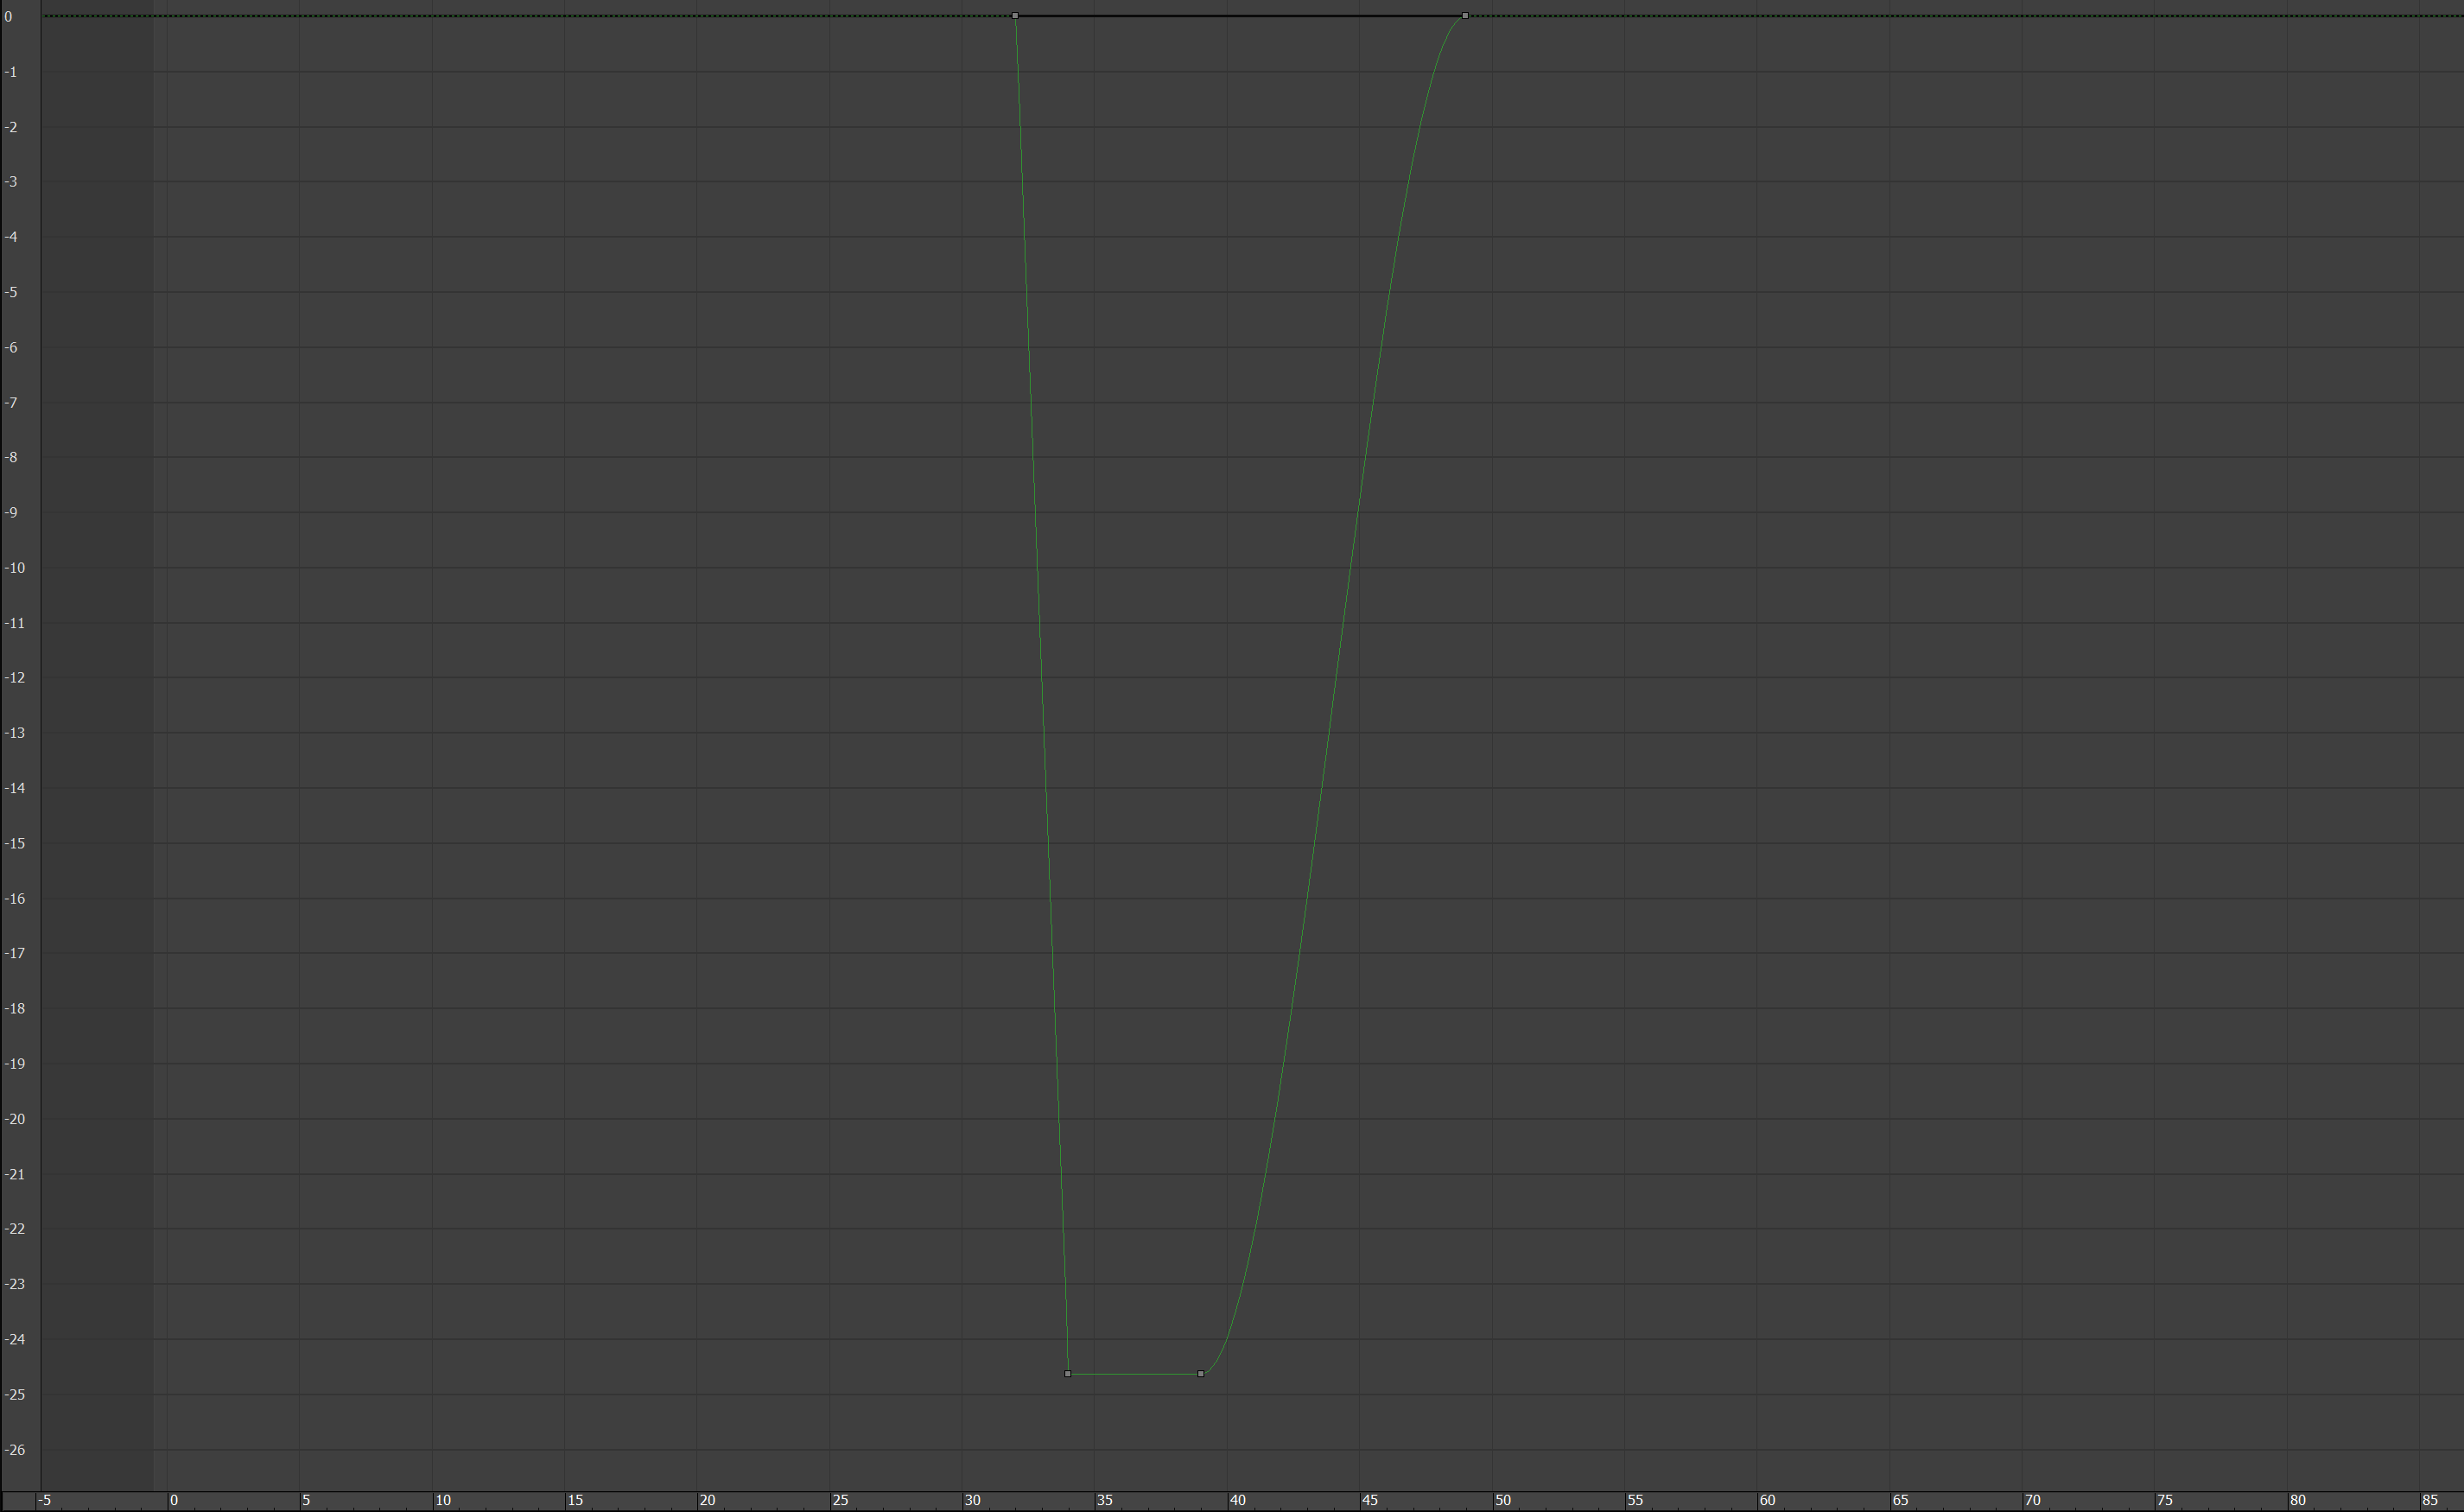
\includegraphics[width=0.8\textwidth]{imagenes/Ejercicio2/corregidas/curvas/green.png}
    \caption{Curva referente a la rotación del vehículo en el eje Y.}
\end{figure}

En cuanto a la curva verde (Rotación en el eje Y), se utiliza para rotar el vehículo durante el cambio de pendiente a la subida de la rampa y para enderezarlo durante el lanzamiento.


\section{Ejercicio 3 - Pelota botando}

En este ejercicio se pide animar una pelota que rebota varias veces sobre una mesa y que finalmente cae al suelo.

\bigskip

La mesa la he realizado usando 5 cubos: uno grande para el tablero y otros 4 del mismo tamaño para hacer las patas. Además, la jerarquía utilizada ha sido de dejar como padre al tablero y como hijos las patas.

\bigskip

En cuanto a la animación, he utilizado un factor de 2 para la altura del rebote y la distancia recorrida entre ellos, lo que significa que en cada salto su altura y distancia se reducen a la mitad. La única excepción a esto es en el primer lanzamiento y en el recorrido horizontal para caer al suelo, ya que al probar a seguirlo el resultado era menos realista. 

\bigskip

El movimiento horizontal podría haberse implementado con menos \textit{keyframes}, pero como he querido simular la pérdida de velocidad en cada acción que realiza la pelota, he necesitado incluir más \textit{keyframes} de manera obligatoria. 

\bigskip

Asimismo, el penúltimo \textit{keyframe} del movimiento horizontal (cuando la pelota va a caer al suelo) puede parecer que no sea necesario, al tener una pendiente muy similar al segmento anterior, pero he deseado simular que ha perdido velocidad después de todos los rebotes, sin seguir el factor de 2, que hacía que perdiera demasiada velocidad. Entonces, tampoco se puede eliminar, al ser una parte importante de la animación.

\bigskip

Esta animación la he realizado usando 10 \textit{keyframes}, que son:

\begin{enumerate}
    \item \textbf{Instante 0:} La pelota se encuentra en el aire, lista para ser lanzada a la mesa.
    \item \textbf{Instante 15:} La pelota ha tocado la mesa por primera vez.
    \item \textbf{Instantes 25, 42, 54:} La pelota ha rebotado y se encuentra en el aire.
    \item \textbf{Instantes 35, 49, 59:} La pelota ha tocado de nuevo el tablero de la mesa.
    \item \textbf{Instante 71:} La pelota se encuentra en el borde de la mesa, justo antes de que se caiga al suelo.
    \item \textbf{Instante 84:} La pelota ha caído y se encuentra en el suelo.
\end{enumerate}

\bigskip

% imagenes con los keyframes
\begin{figure}[H]
    \centering
    \begin{subfigure}[H]{0.48\textwidth}
        \centering
        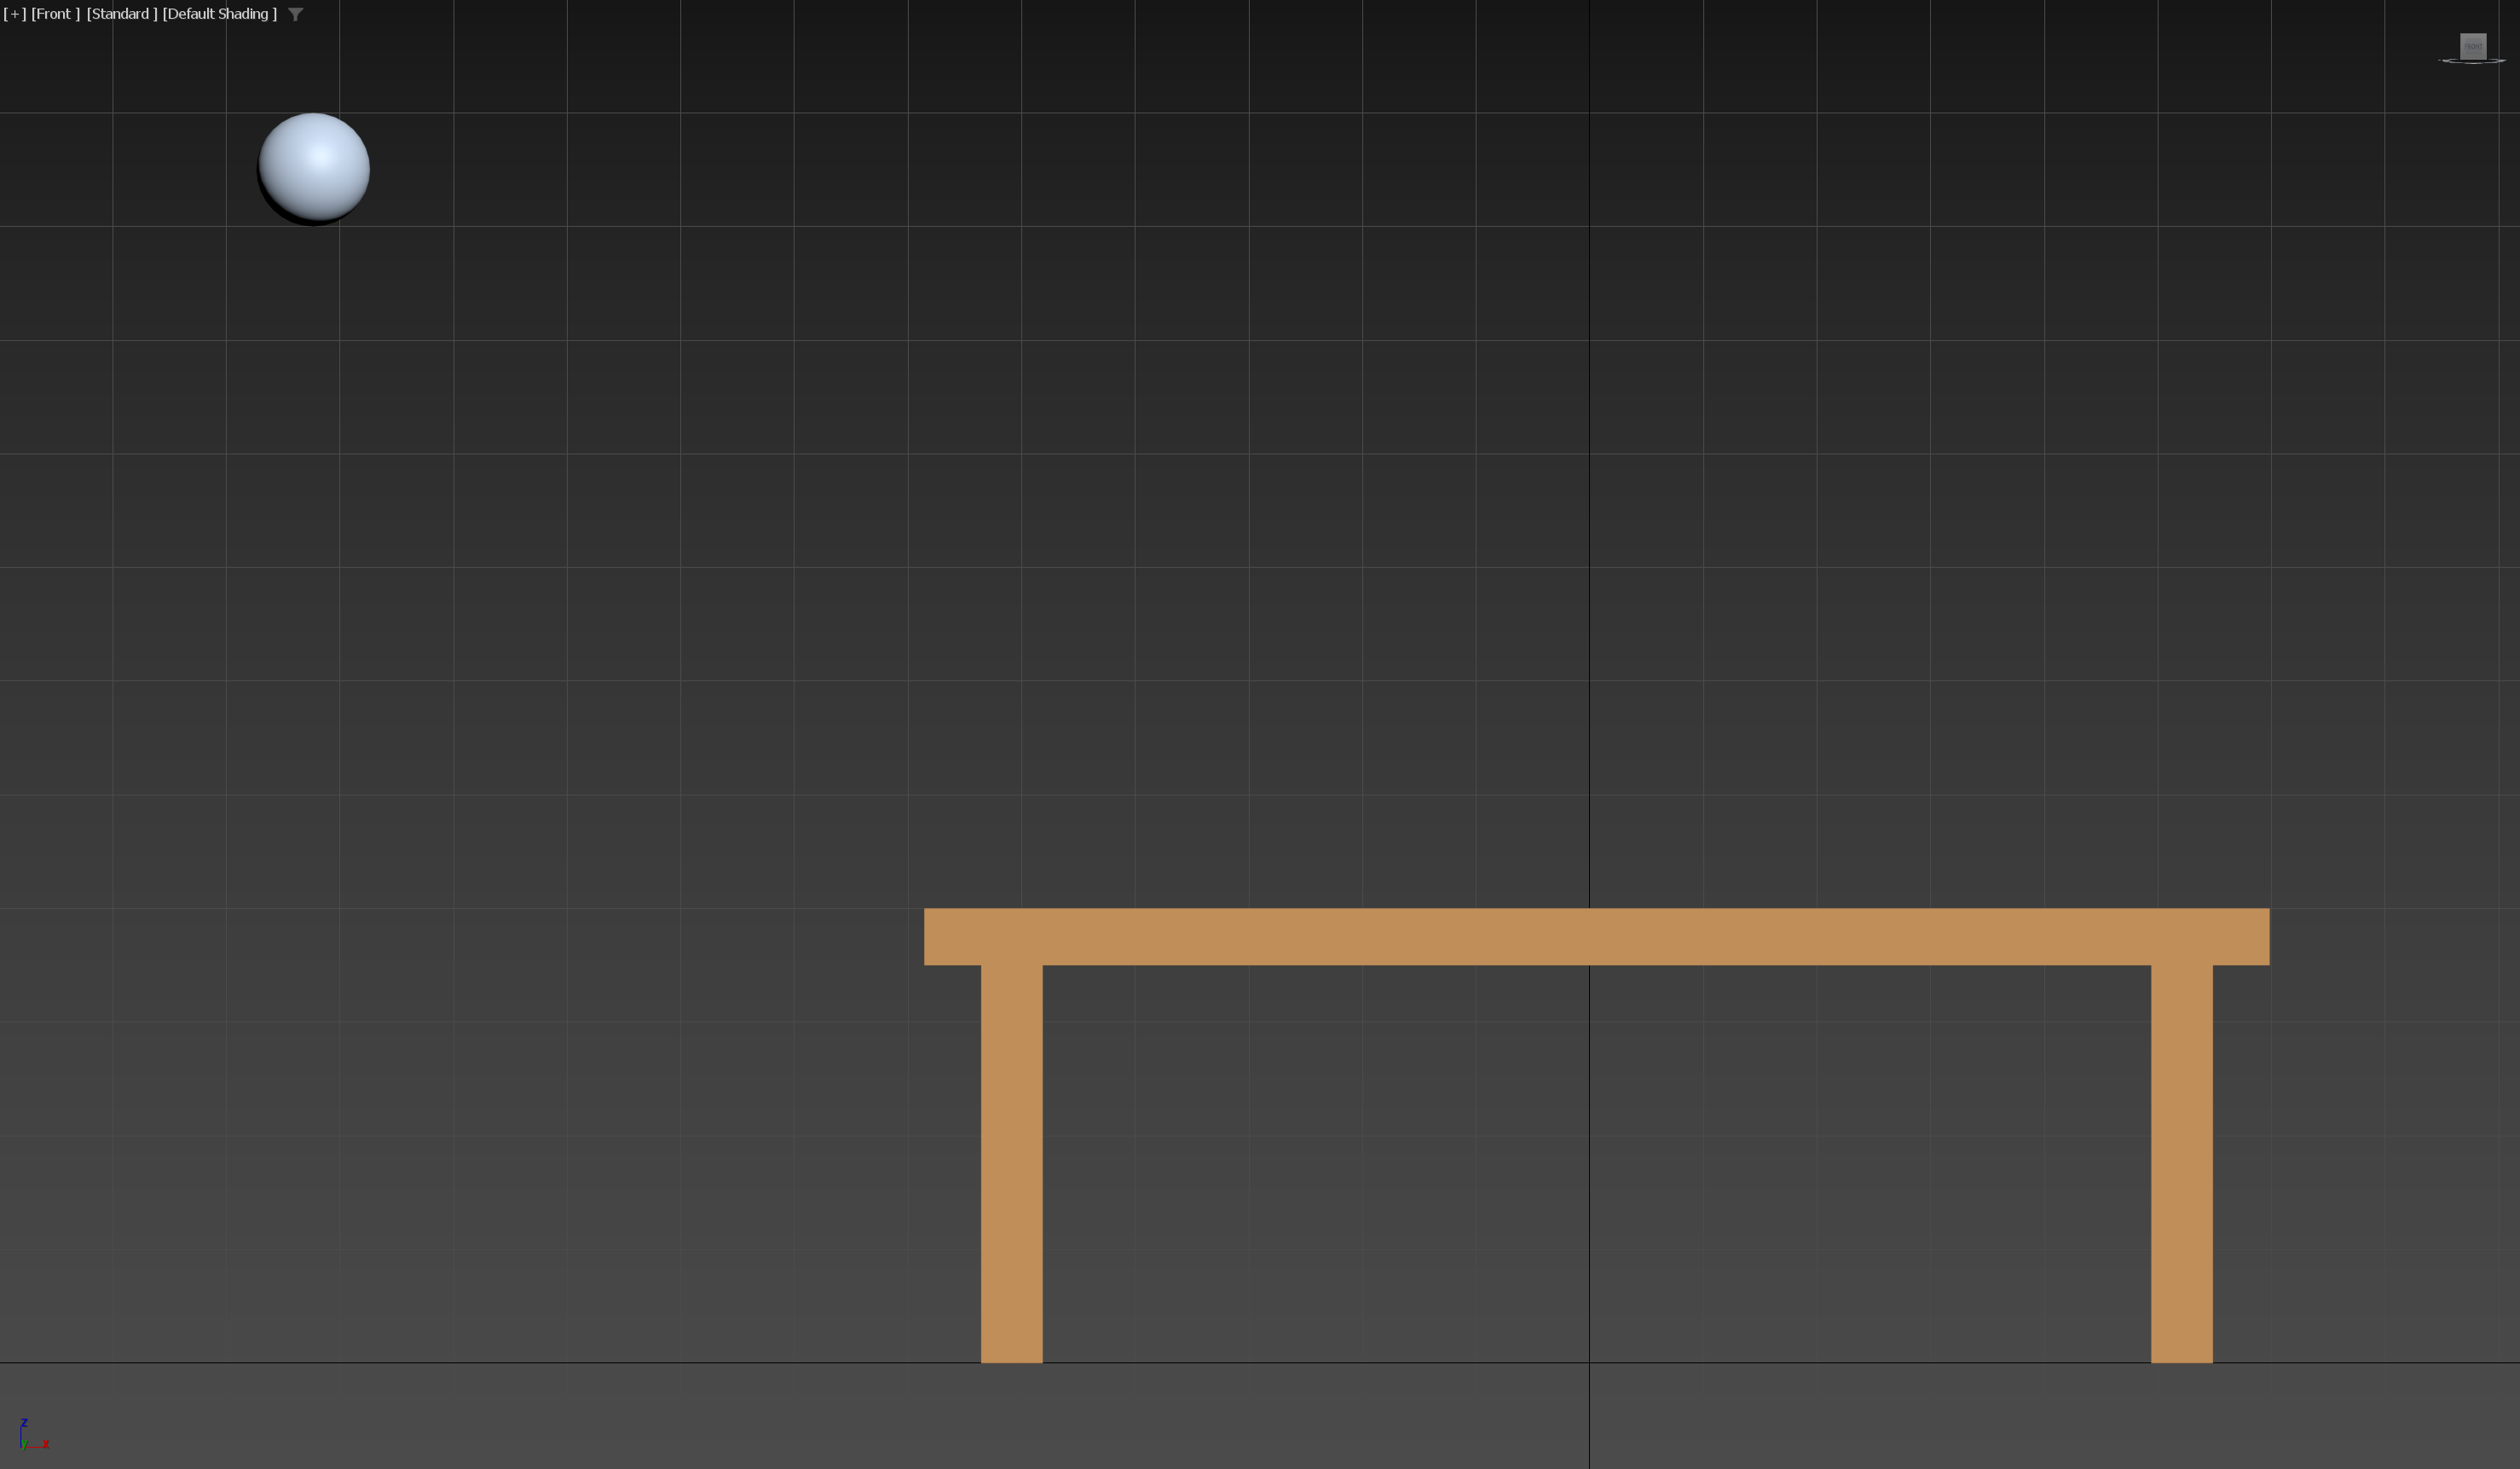
\includegraphics[width=\textwidth]{imagenes/Ejercicio3/keyframes/0.png}
        \caption{Pelota en el instante 0.}
    \end{subfigure}
    \hfill
    \begin{subfigure}[H]{0.48\textwidth}
        \centering
        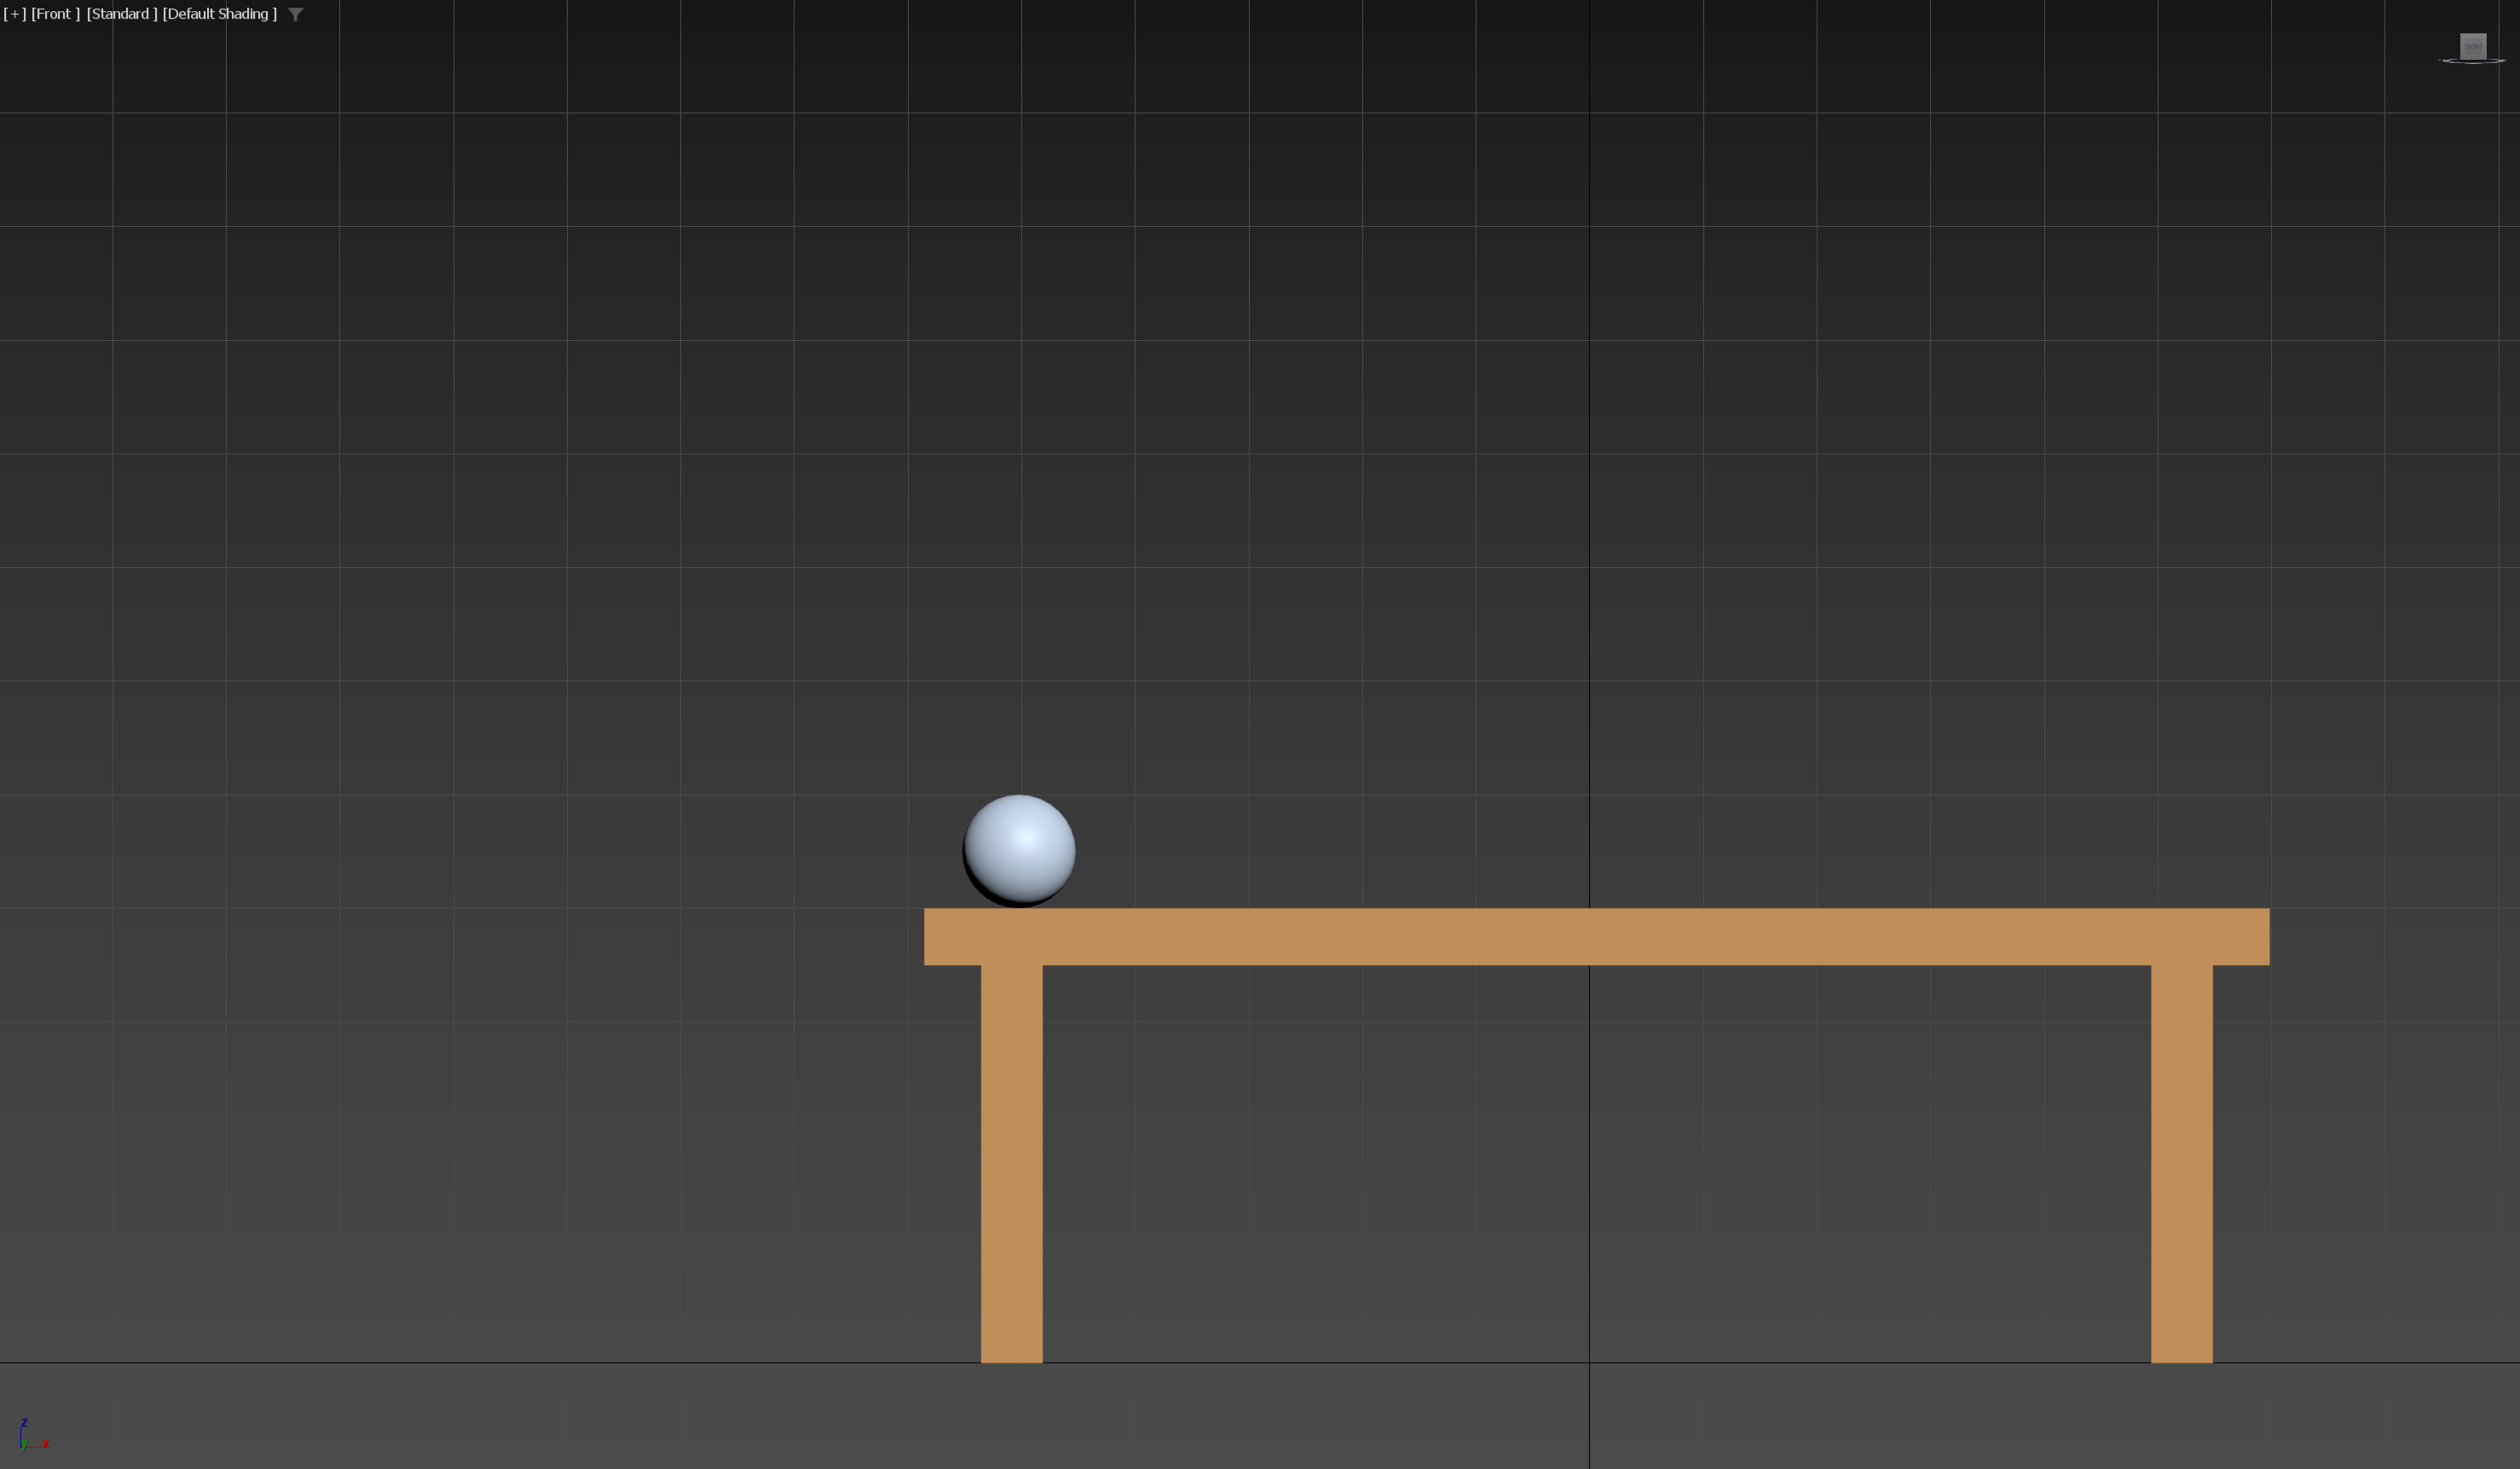
\includegraphics[width=\textwidth]{imagenes/Ejercicio3/keyframes/15.png}
        \caption{Pelota en el instante 15.}
    \end{subfigure}
    % \hfill
    \par\bigskip
    \begin{subfigure}[H]{0.48\textwidth}
        \centering
        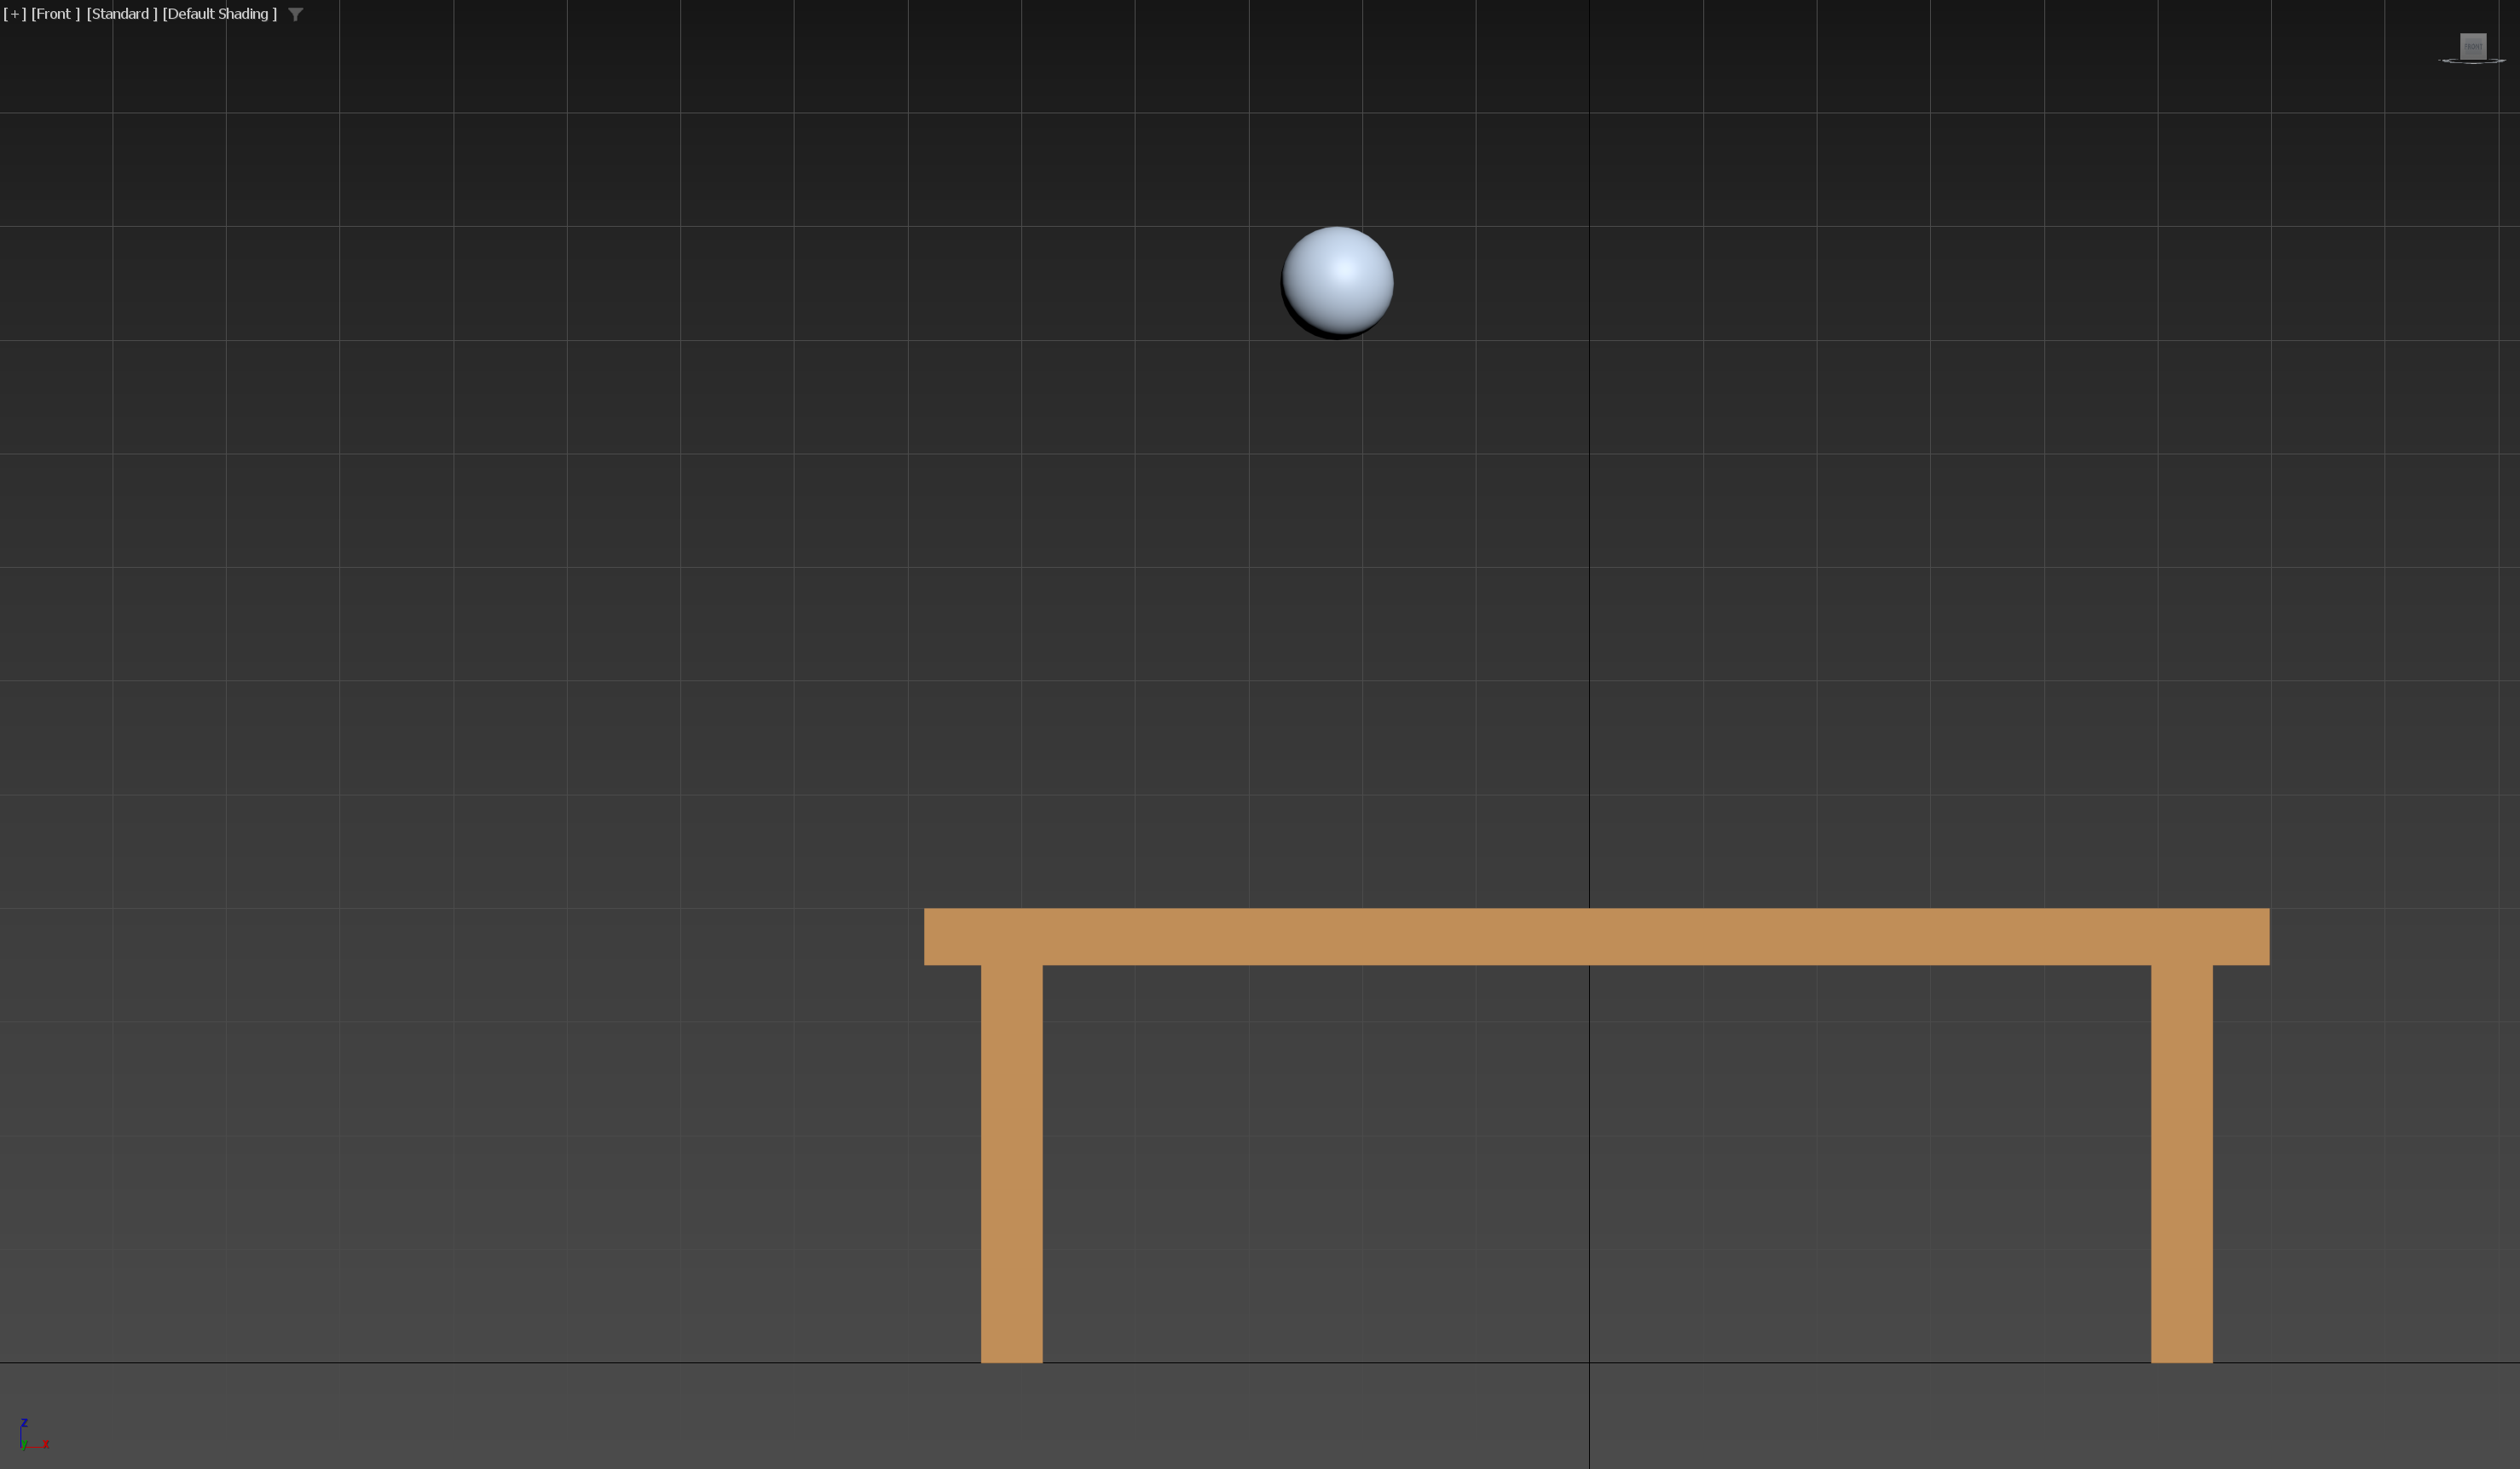
\includegraphics[width=\textwidth]{imagenes/Ejercicio3/keyframes/25.png}
        \caption{Pelota en el instante 25.}
    \end{subfigure}
    \hfill
    \begin{subfigure}[H]{0.48\textwidth}
        \centering
        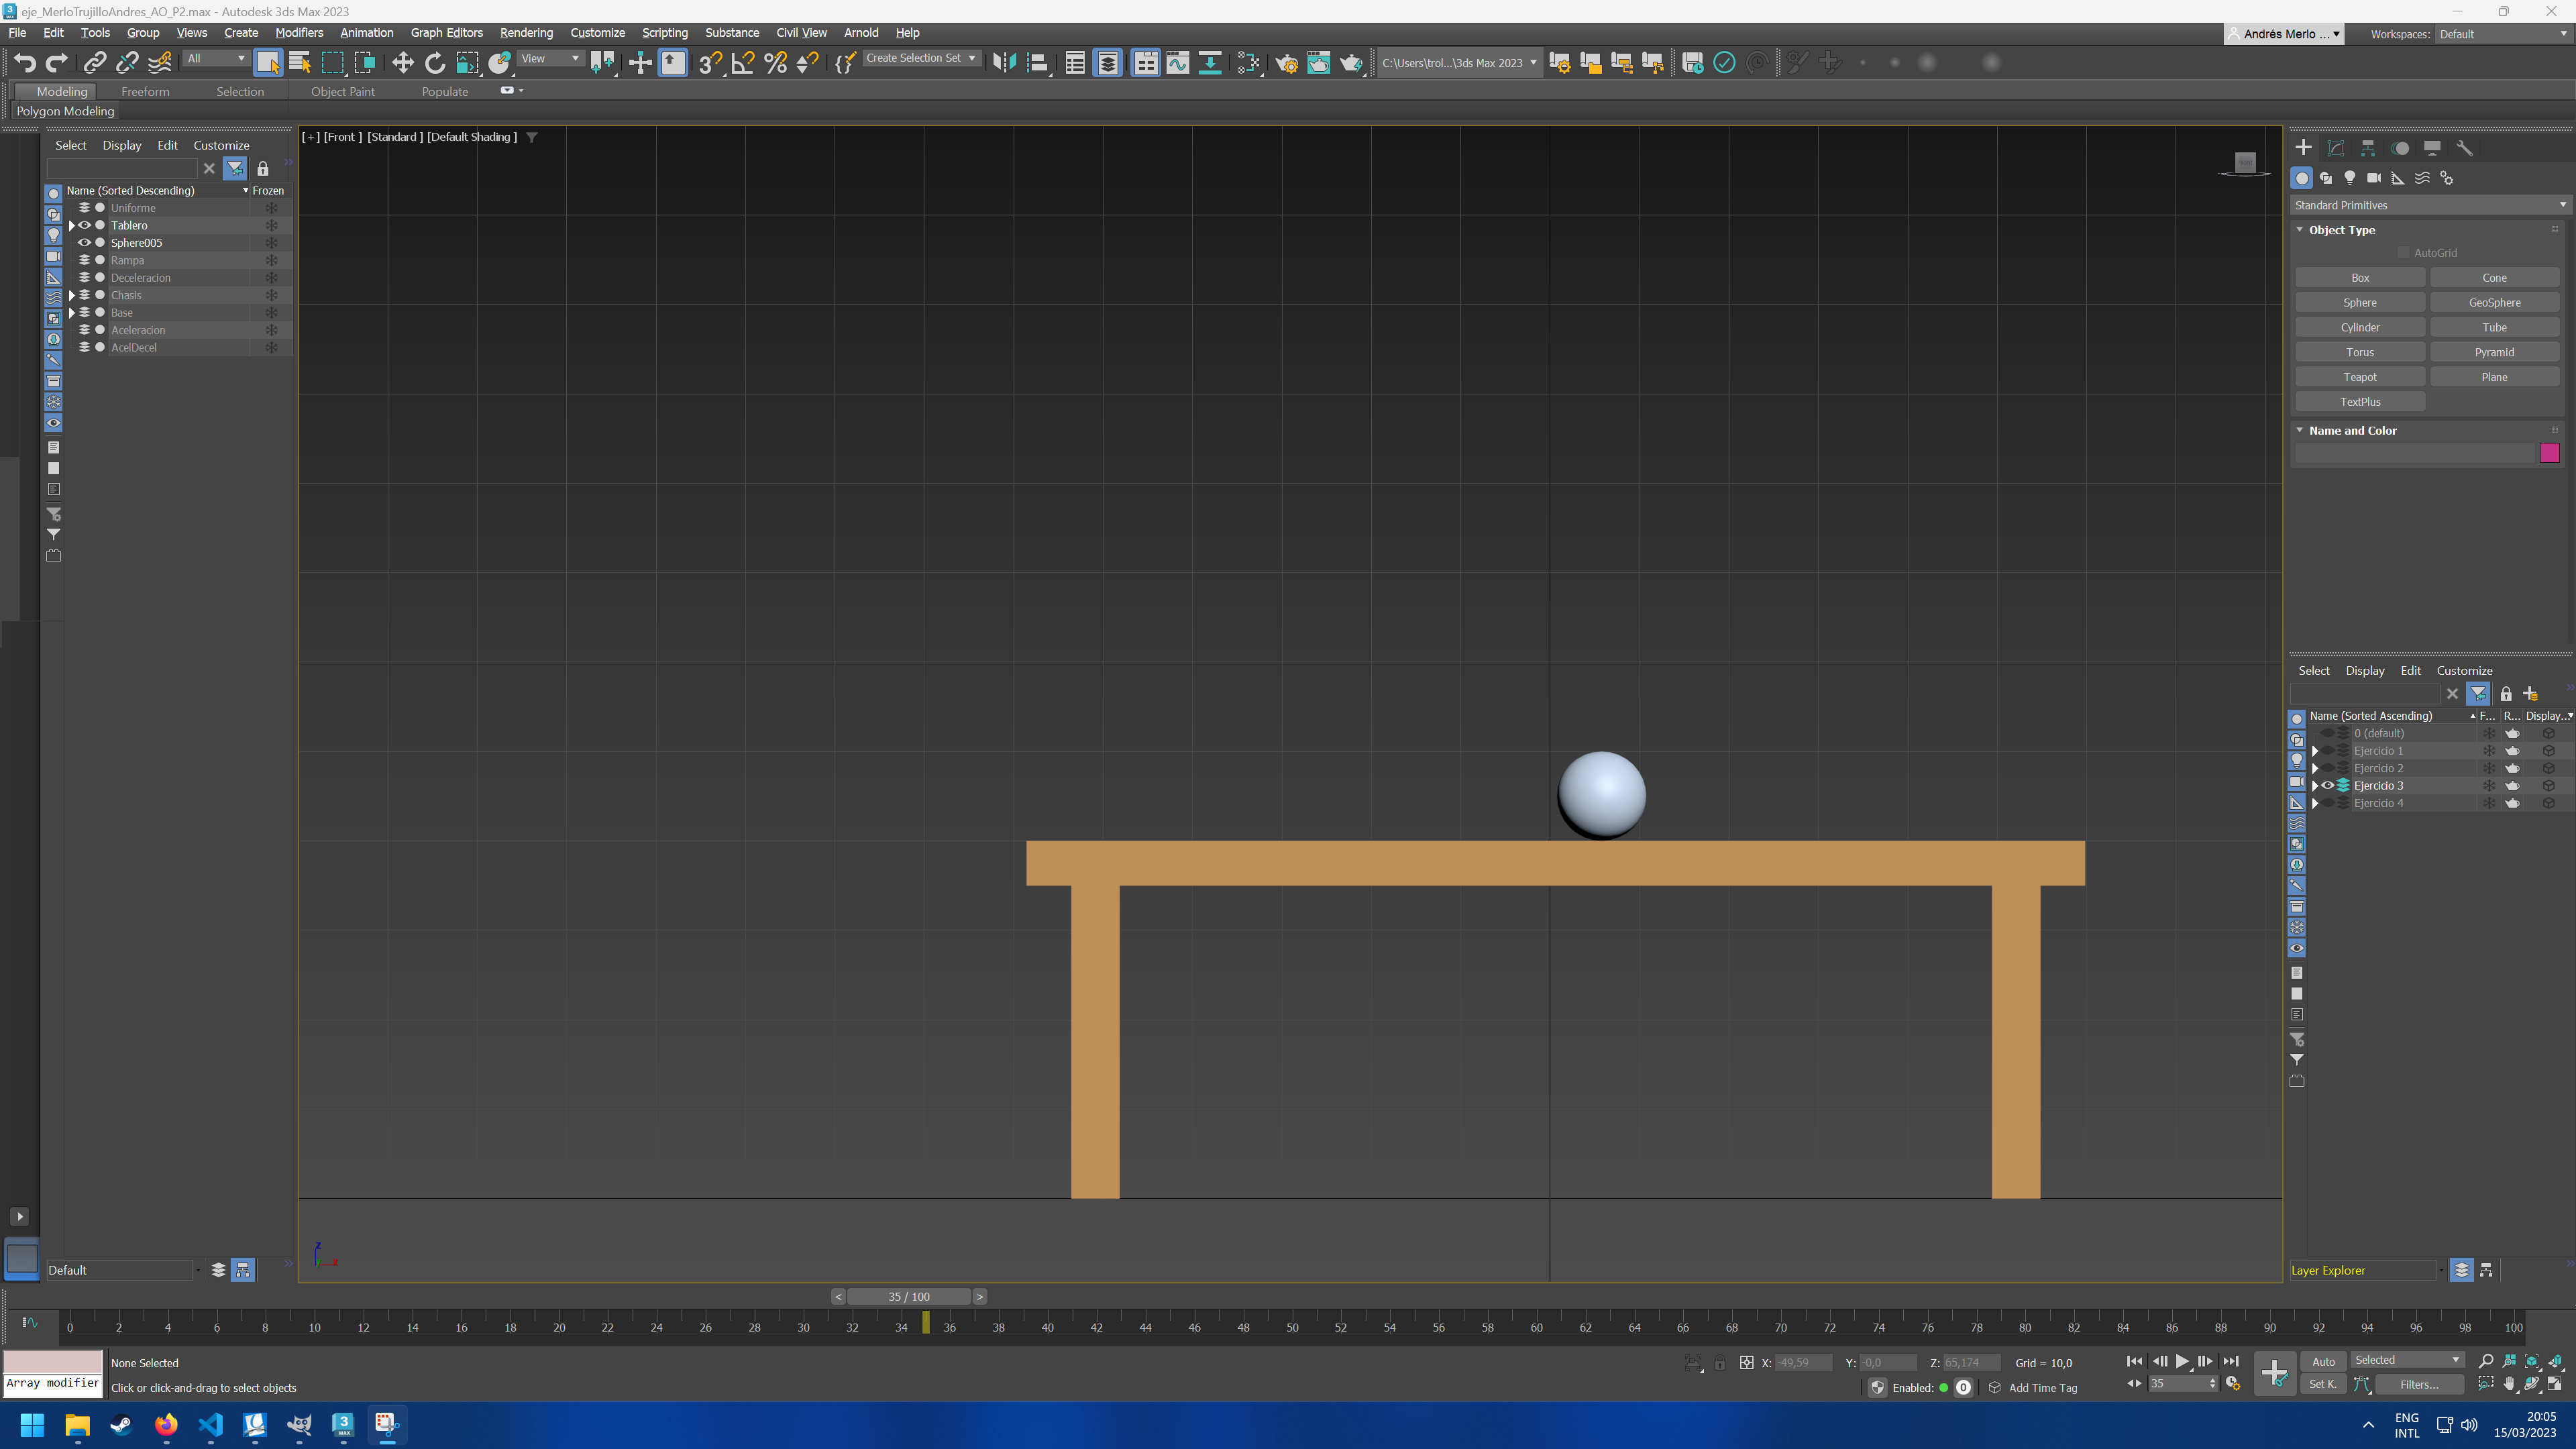
\includegraphics[width=\textwidth]{imagenes/Ejercicio3/keyframes/35.png}
        \caption{Pelota en el instante 35.}
    \end{subfigure}
    % \hfill
    \par\bigskip
    \begin{subfigure}[H]{0.48\textwidth}
        \centering
        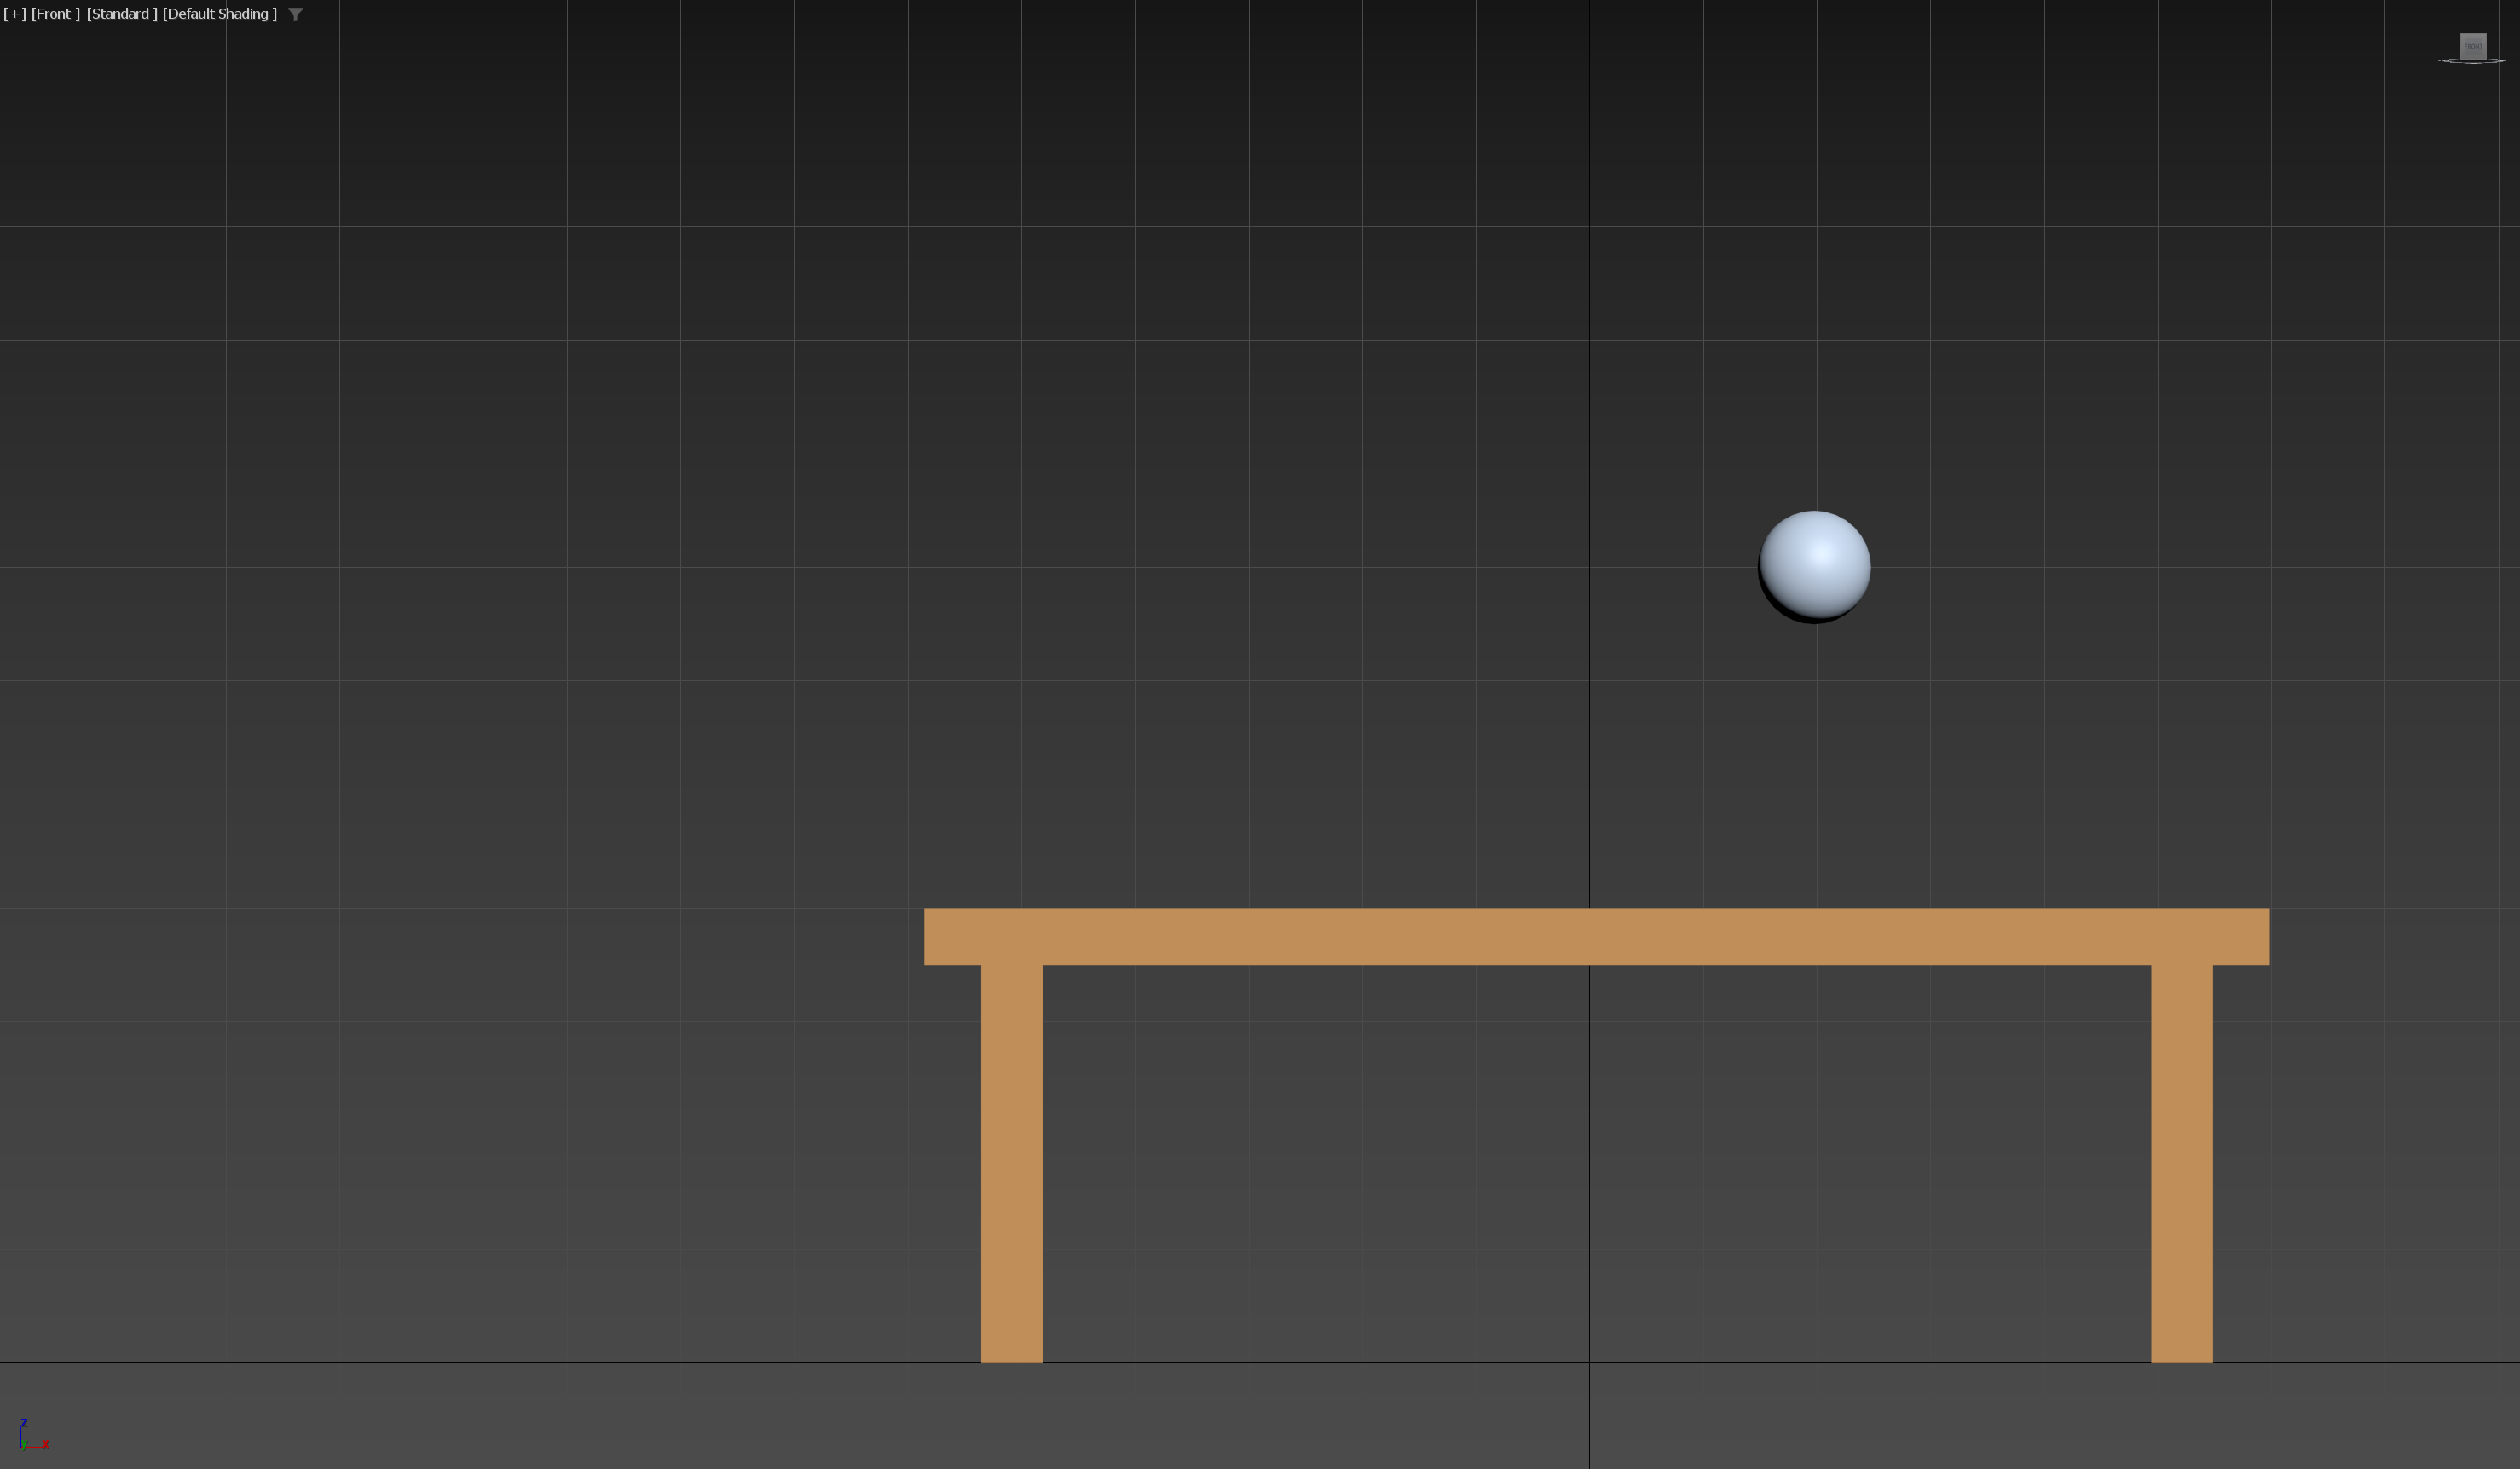
\includegraphics[width=\textwidth]{imagenes/Ejercicio3/keyframes/42.png}
        \caption{Pelota en el instante 42.}
    \end{subfigure}
    \hfill
    \begin{subfigure}[H]{0.48\textwidth}
        \centering
        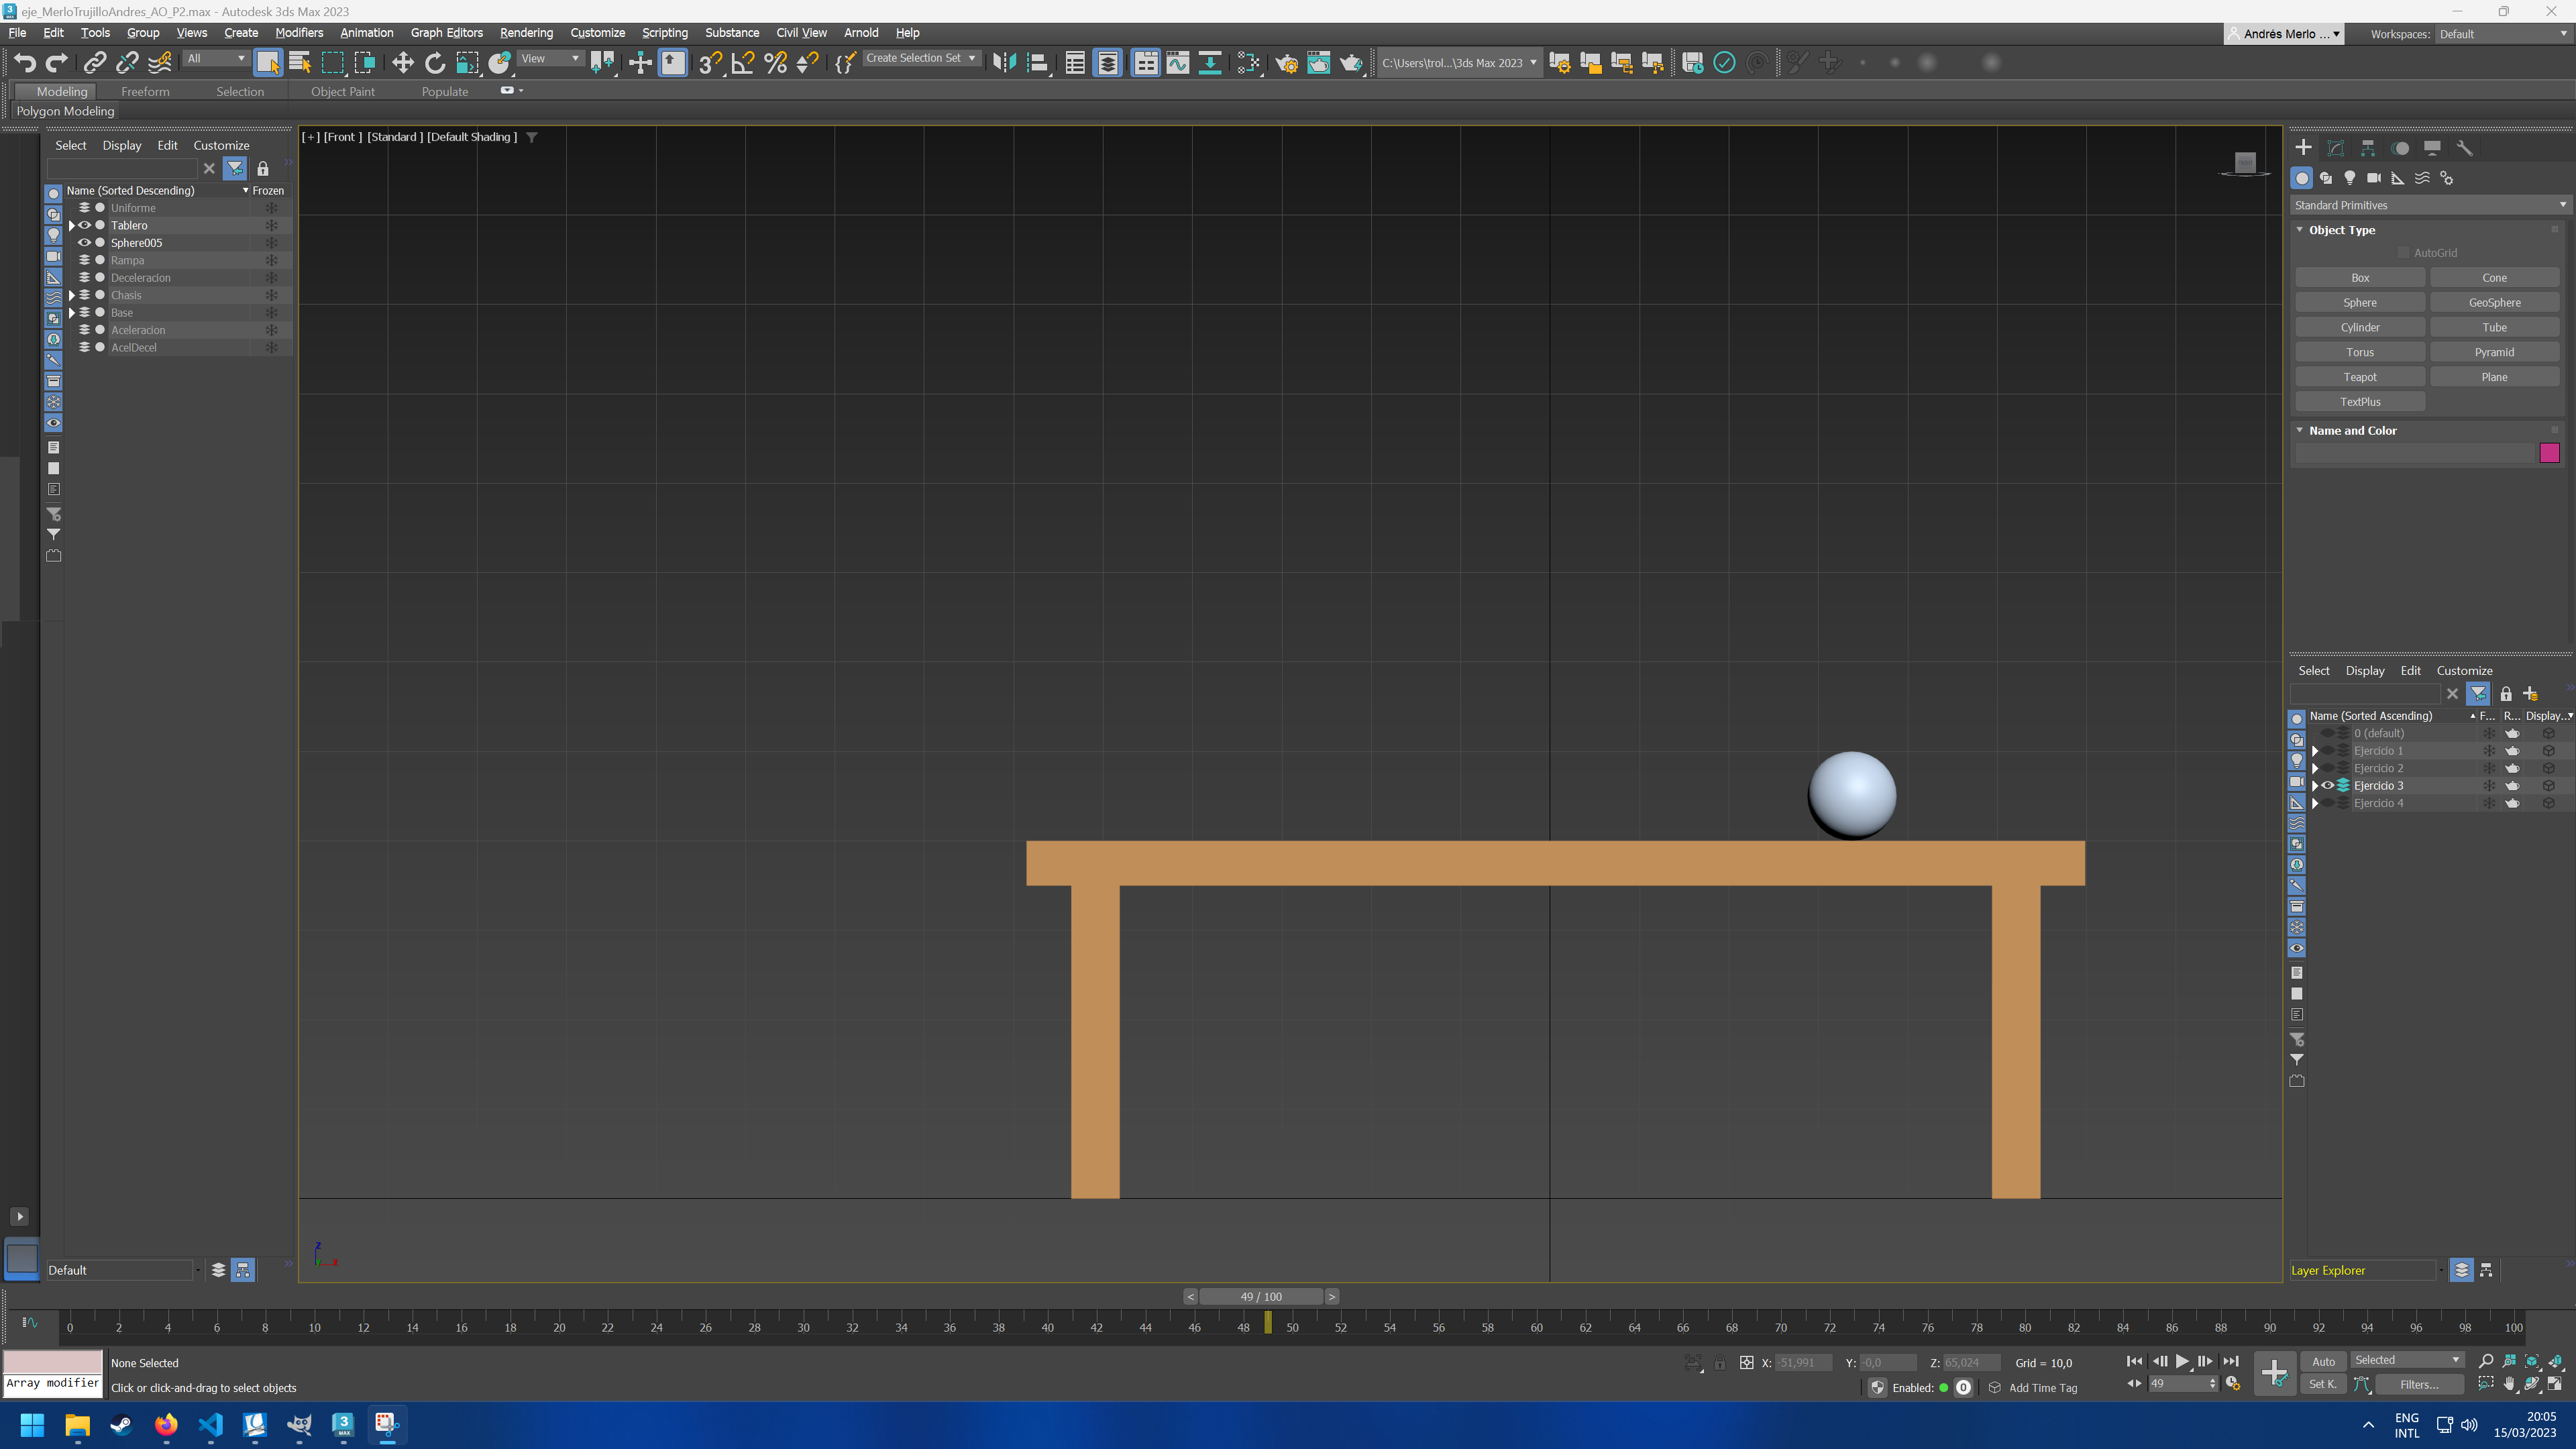
\includegraphics[width=\textwidth]{imagenes/Ejercicio3/keyframes/49.png}
        \caption{Pelota en el instante 49.}
    \end{subfigure}
    % \hfill
    \par\bigskip
    \begin{subfigure}[H]{0.48\textwidth}
        \centering
        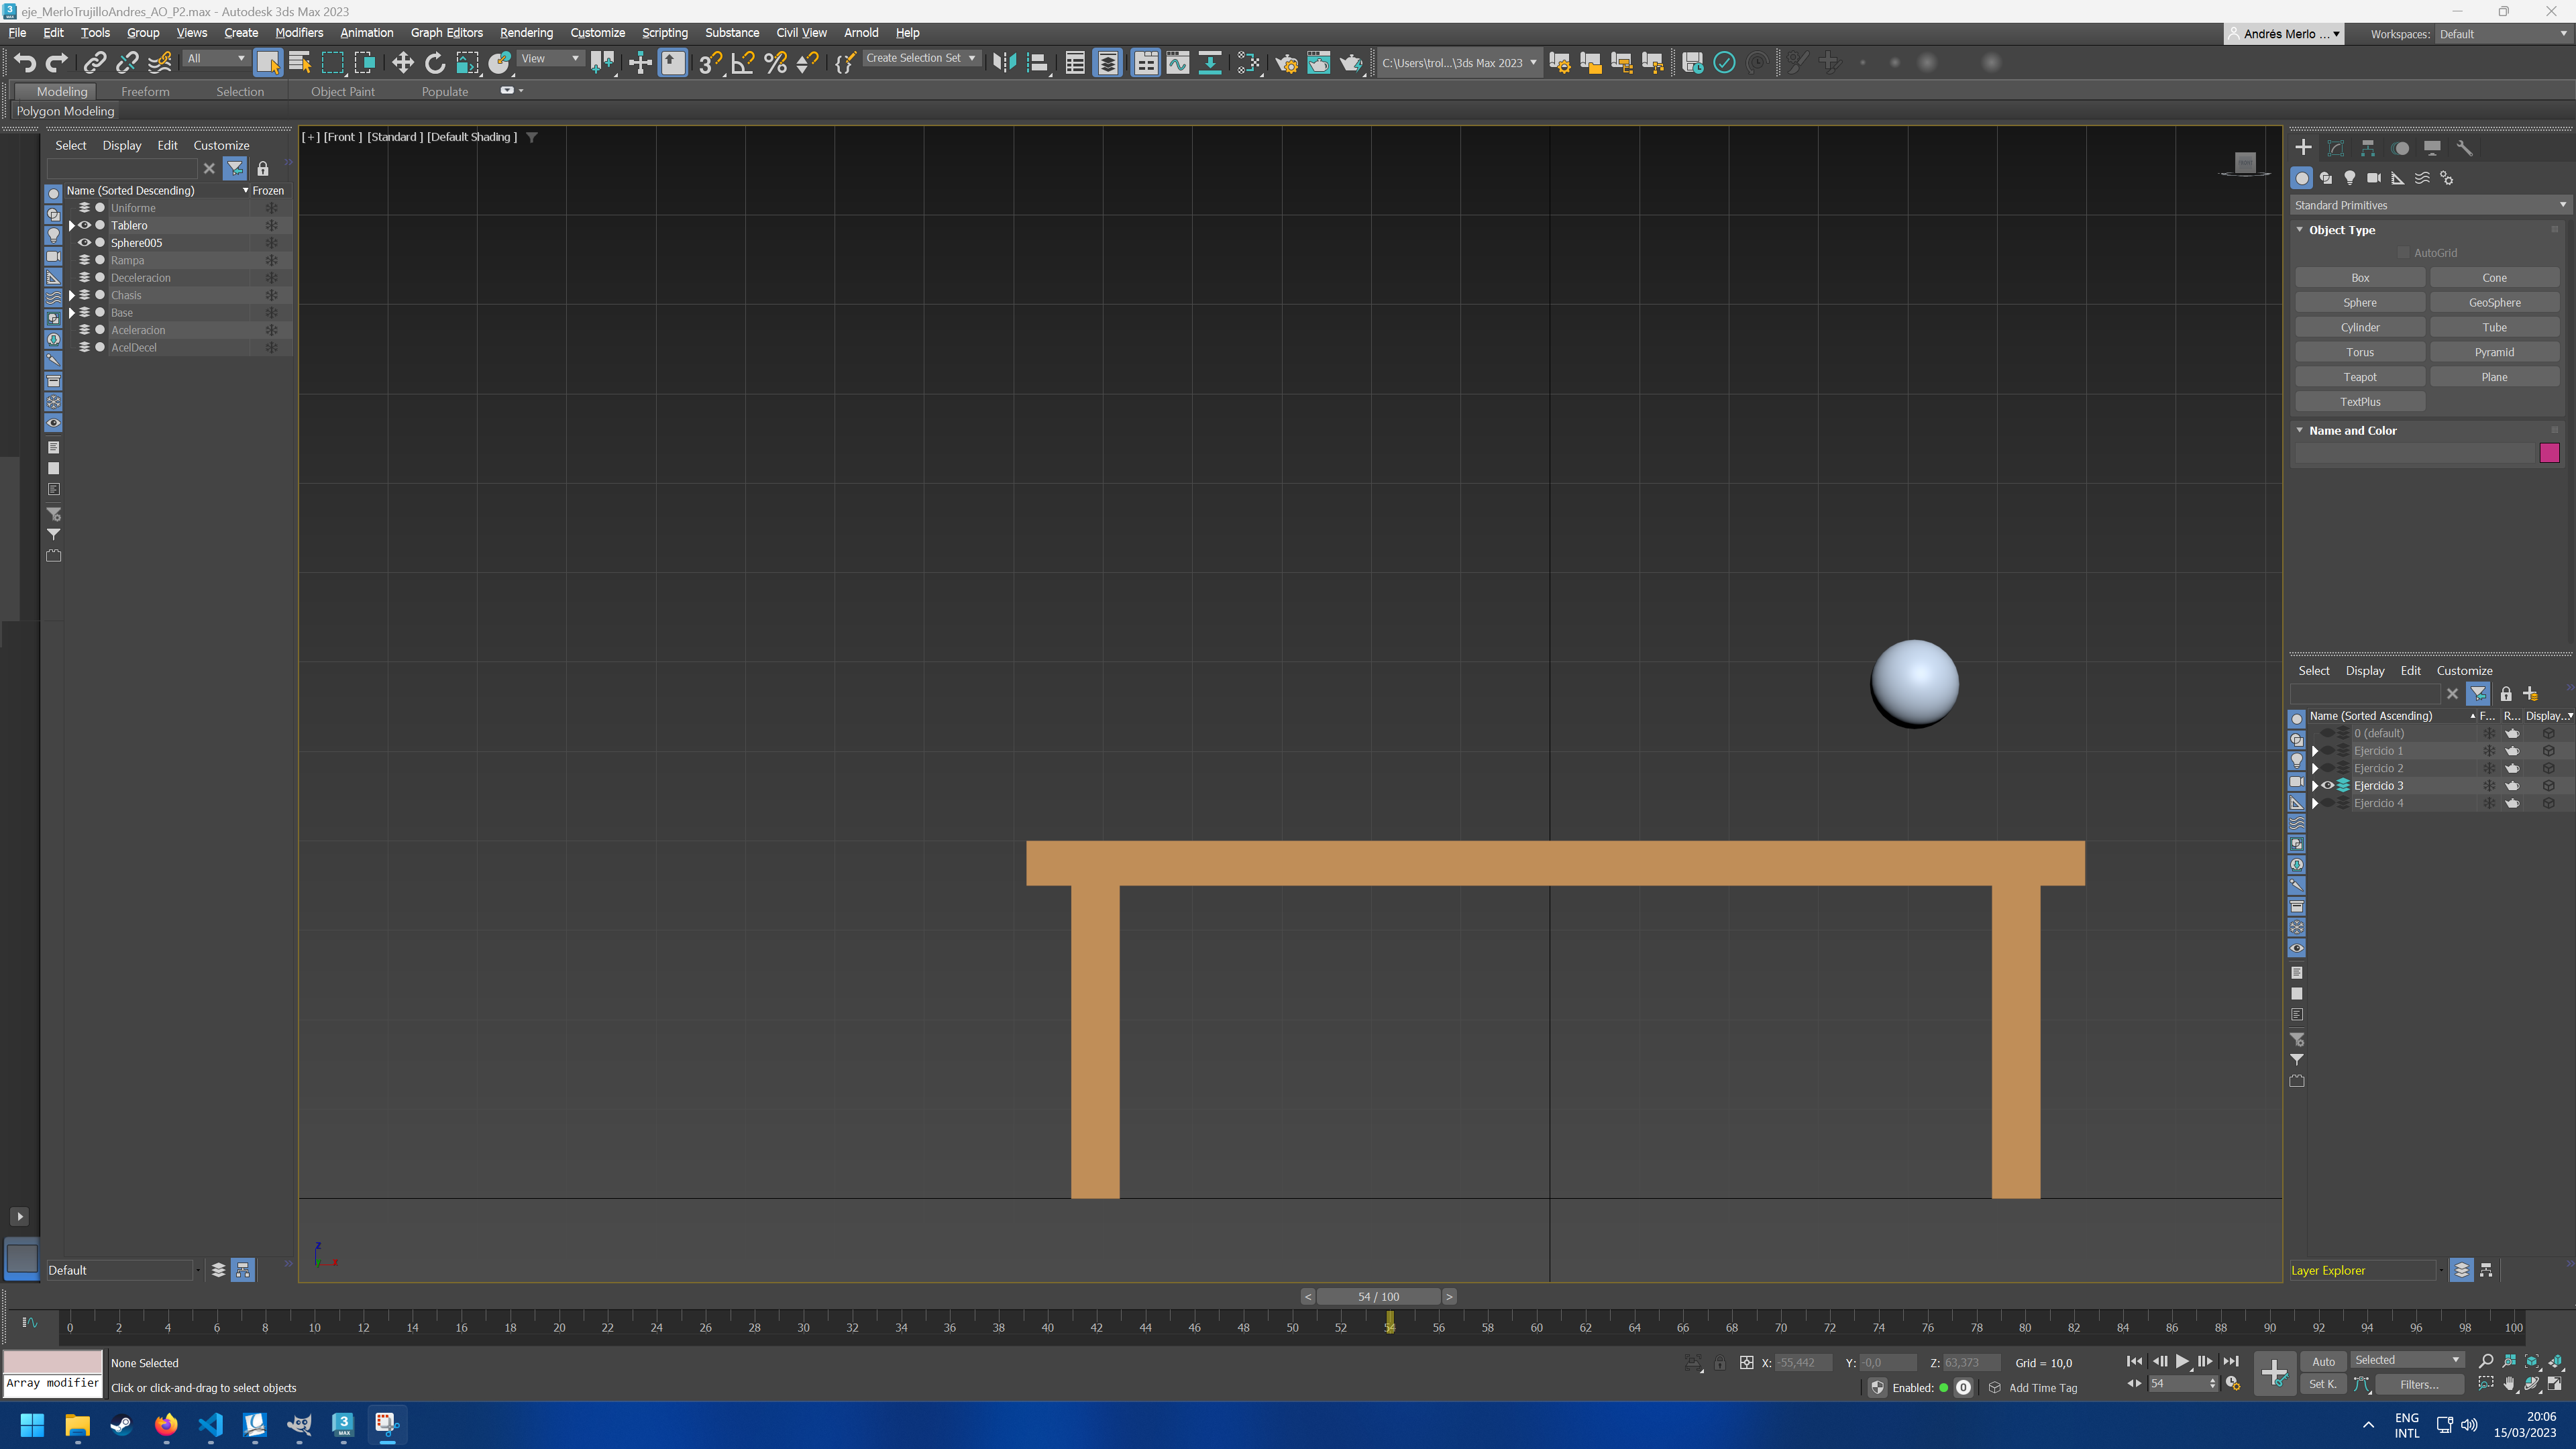
\includegraphics[width=\textwidth]{imagenes/Ejercicio3/keyframes/54.png}
        \caption{Pelota en el instante 54.}
    \end{subfigure}
    \hfill
    \begin{subfigure}[H]{0.48\textwidth}
        \centering
        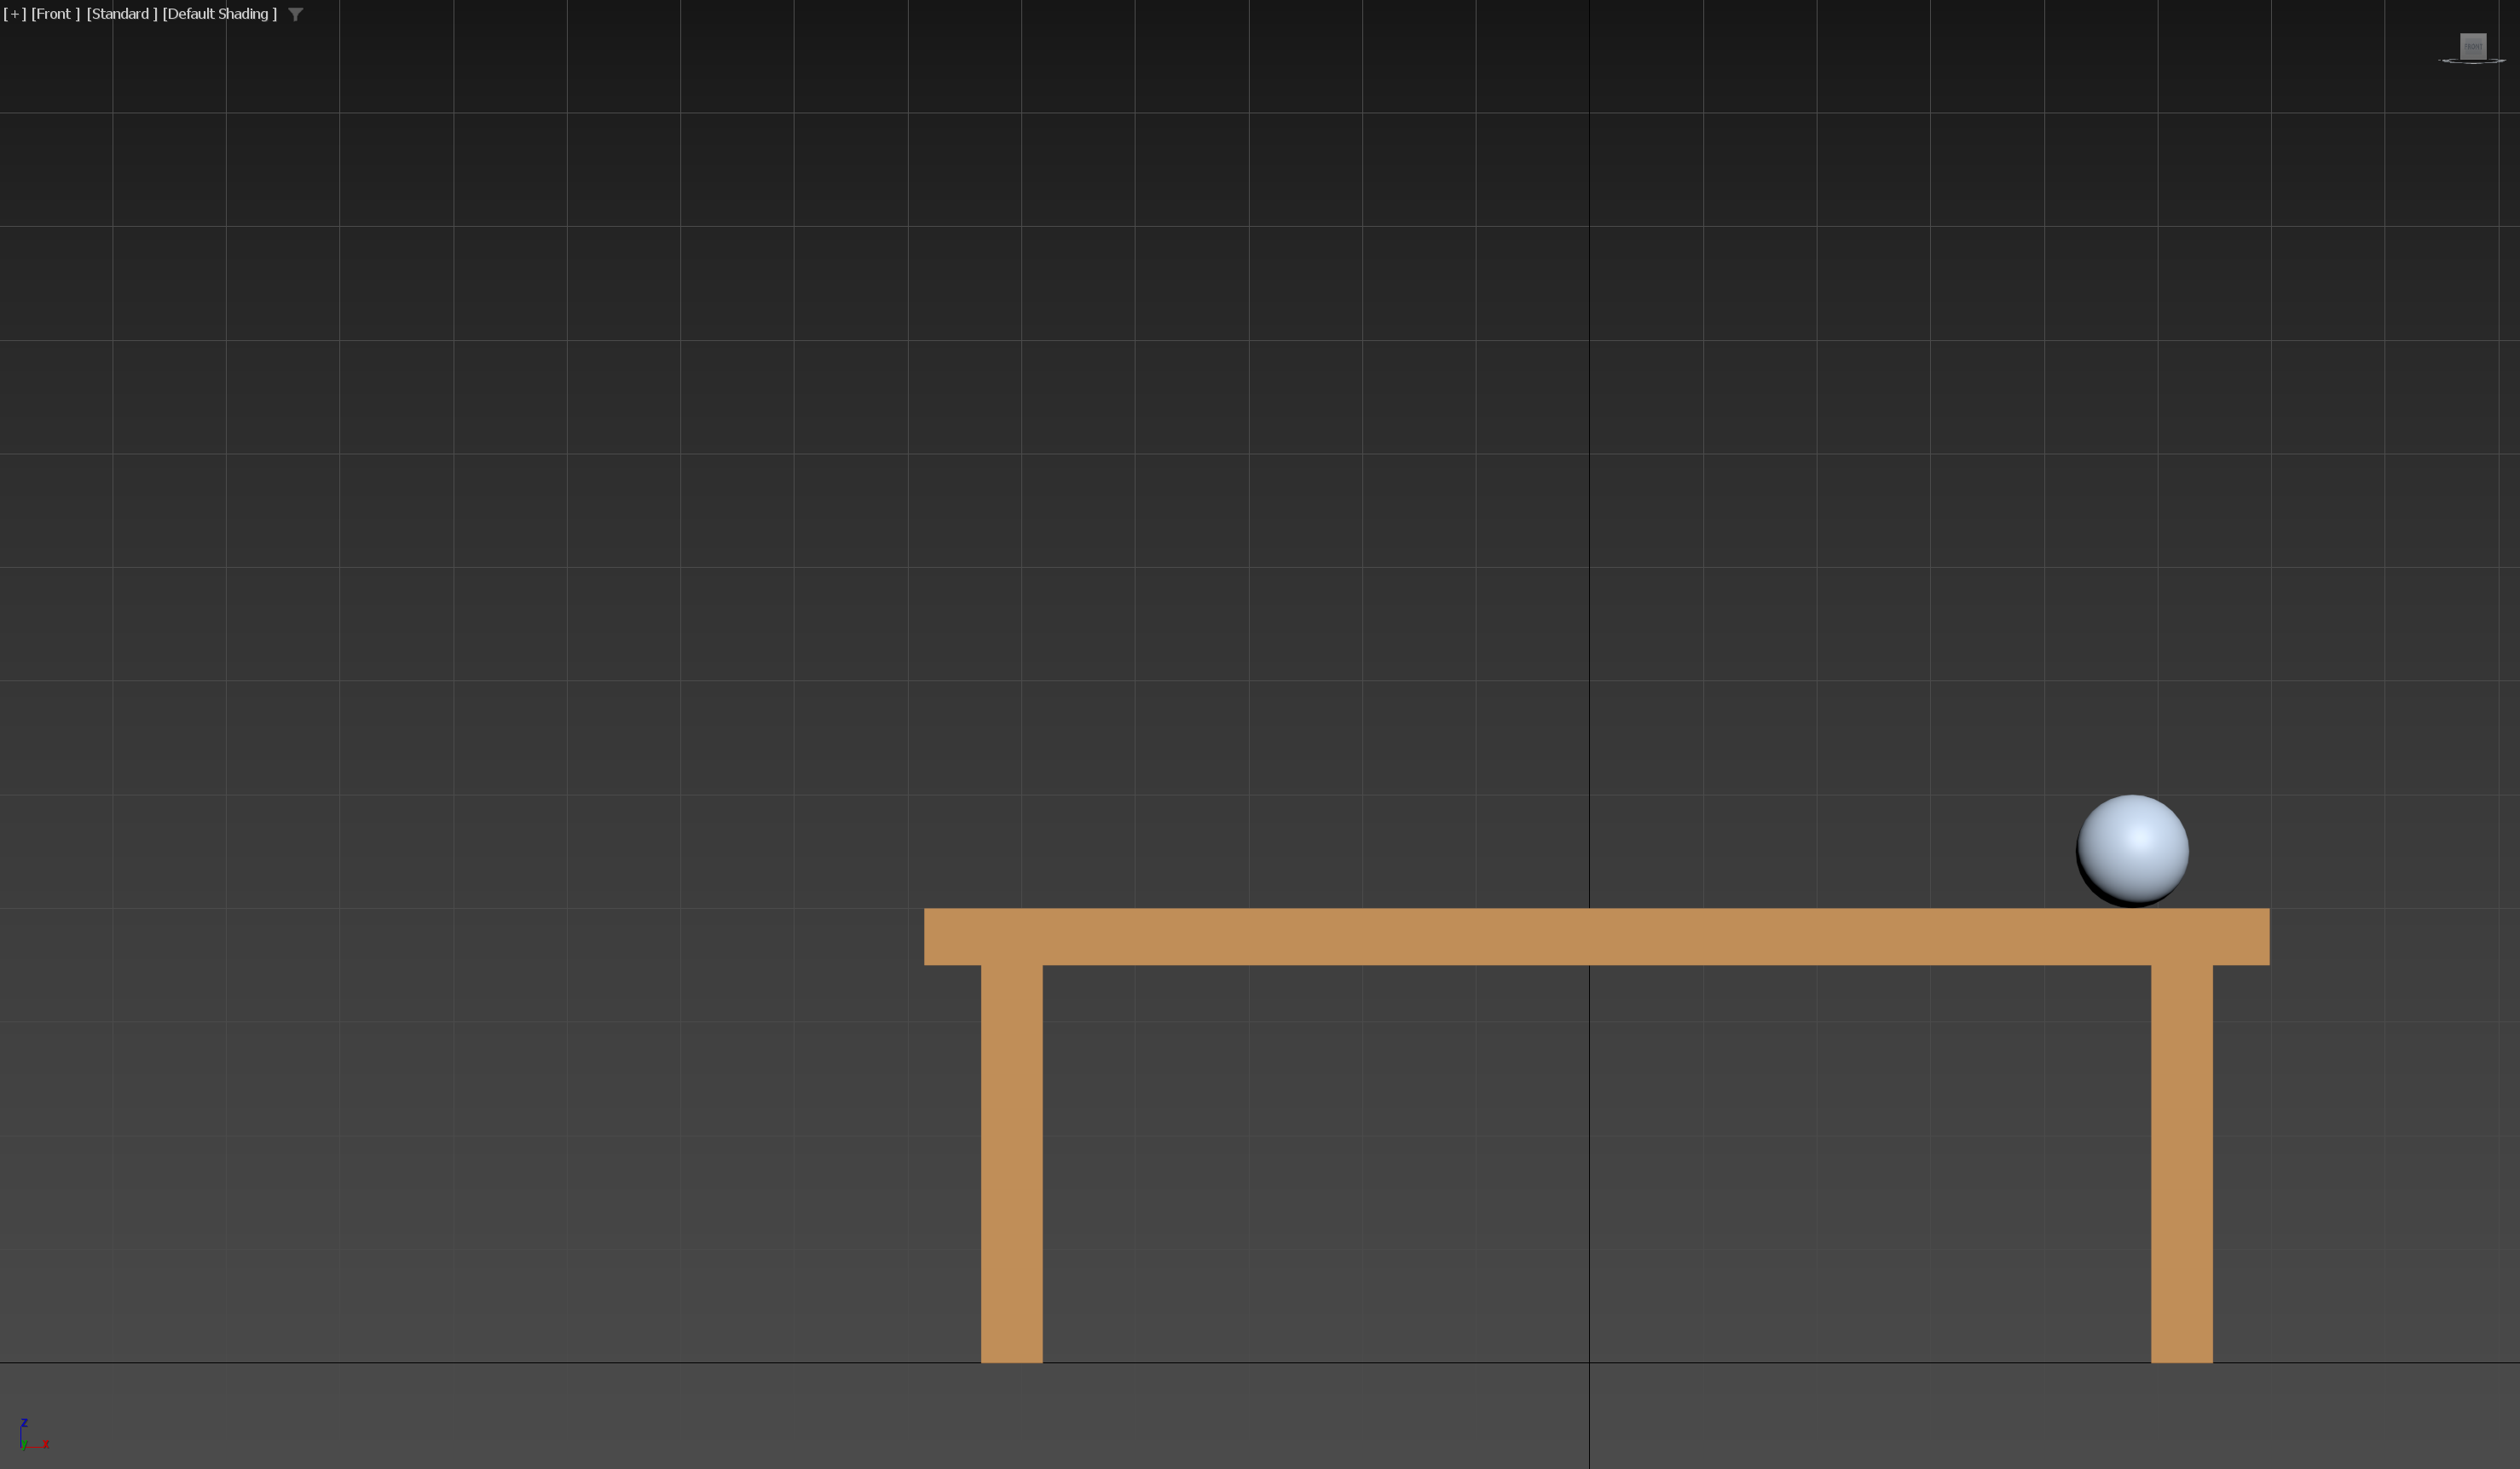
\includegraphics[width=\textwidth]{imagenes/Ejercicio3/keyframes/59.png}
        \caption{Pelota en el instante 59.}
    \end{subfigure}
    % \hfill
\end{figure}

\newpage
\begin{figure}[H]\ContinuedFloat
    \centering
    \begin{subfigure}[H]{0.48\textwidth}
        \centering
        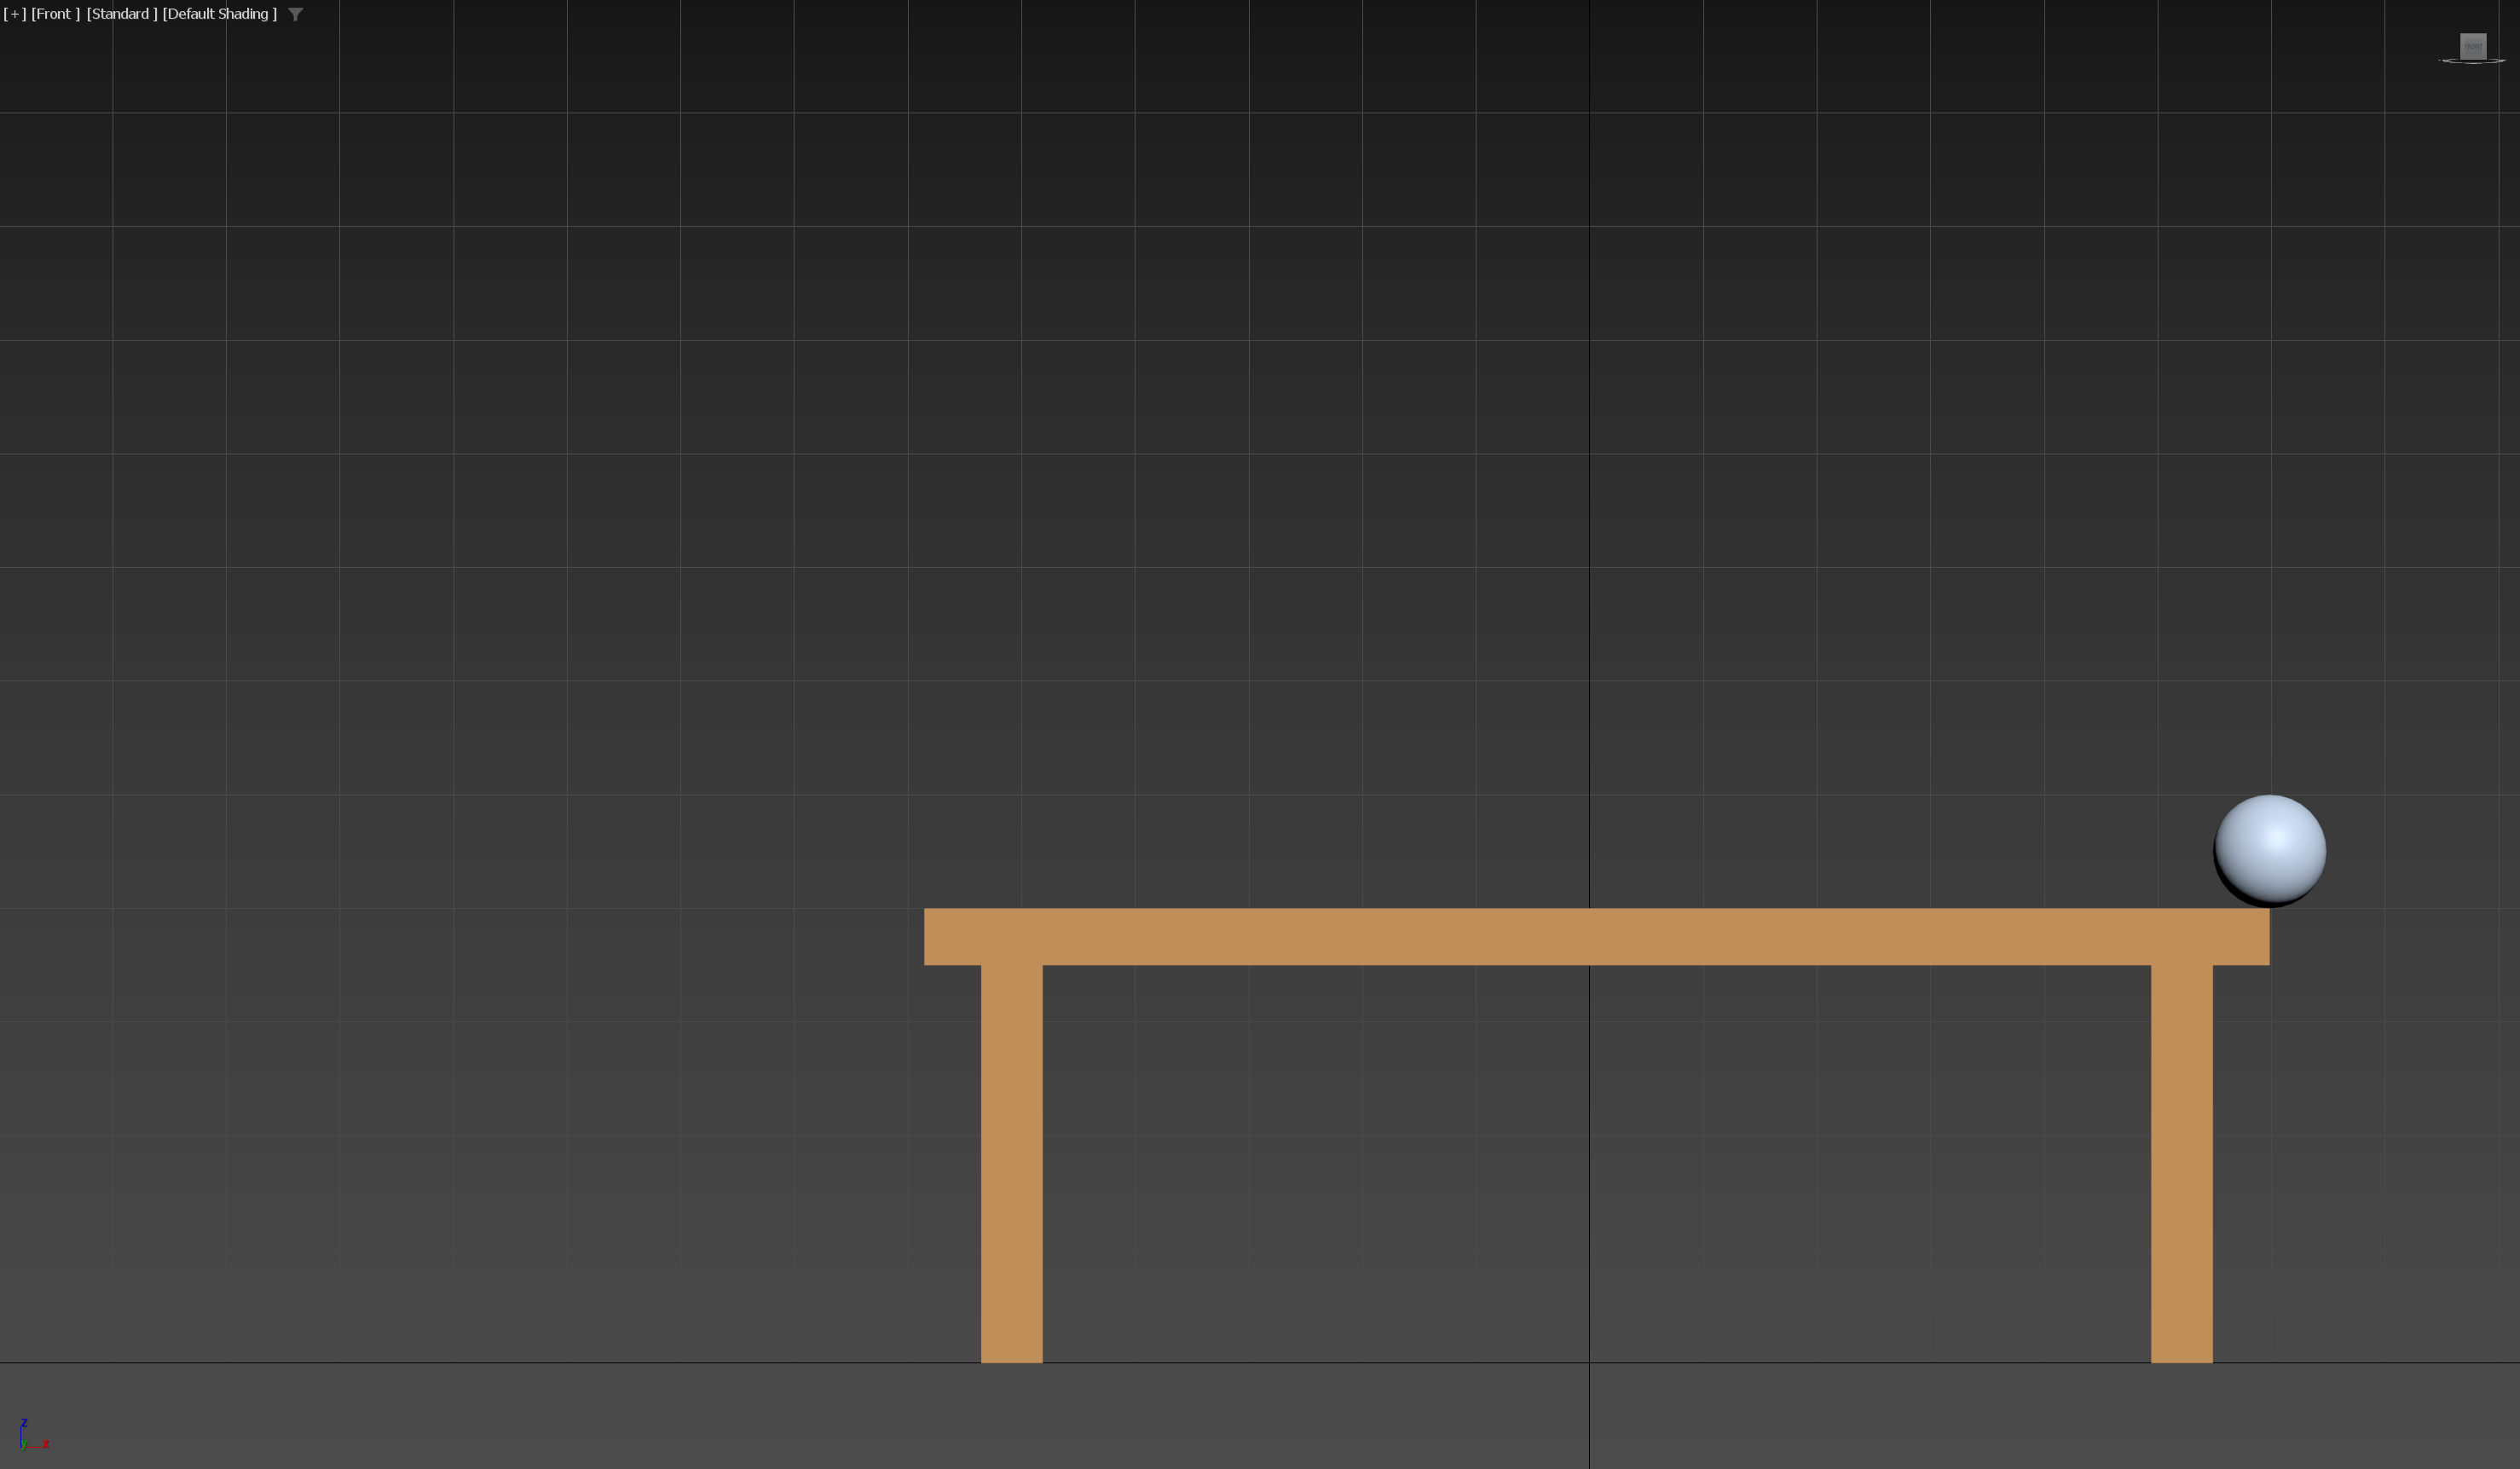
\includegraphics[width=\textwidth]{imagenes/Ejercicio3/keyframes/71.png}
        % \setcounter{subfigure}{9}
        \caption{Pelota en el instante 71.}
    \end{subfigure}
    \hfill
    \begin{subfigure}[H]{0.48\textwidth}
        \centering
        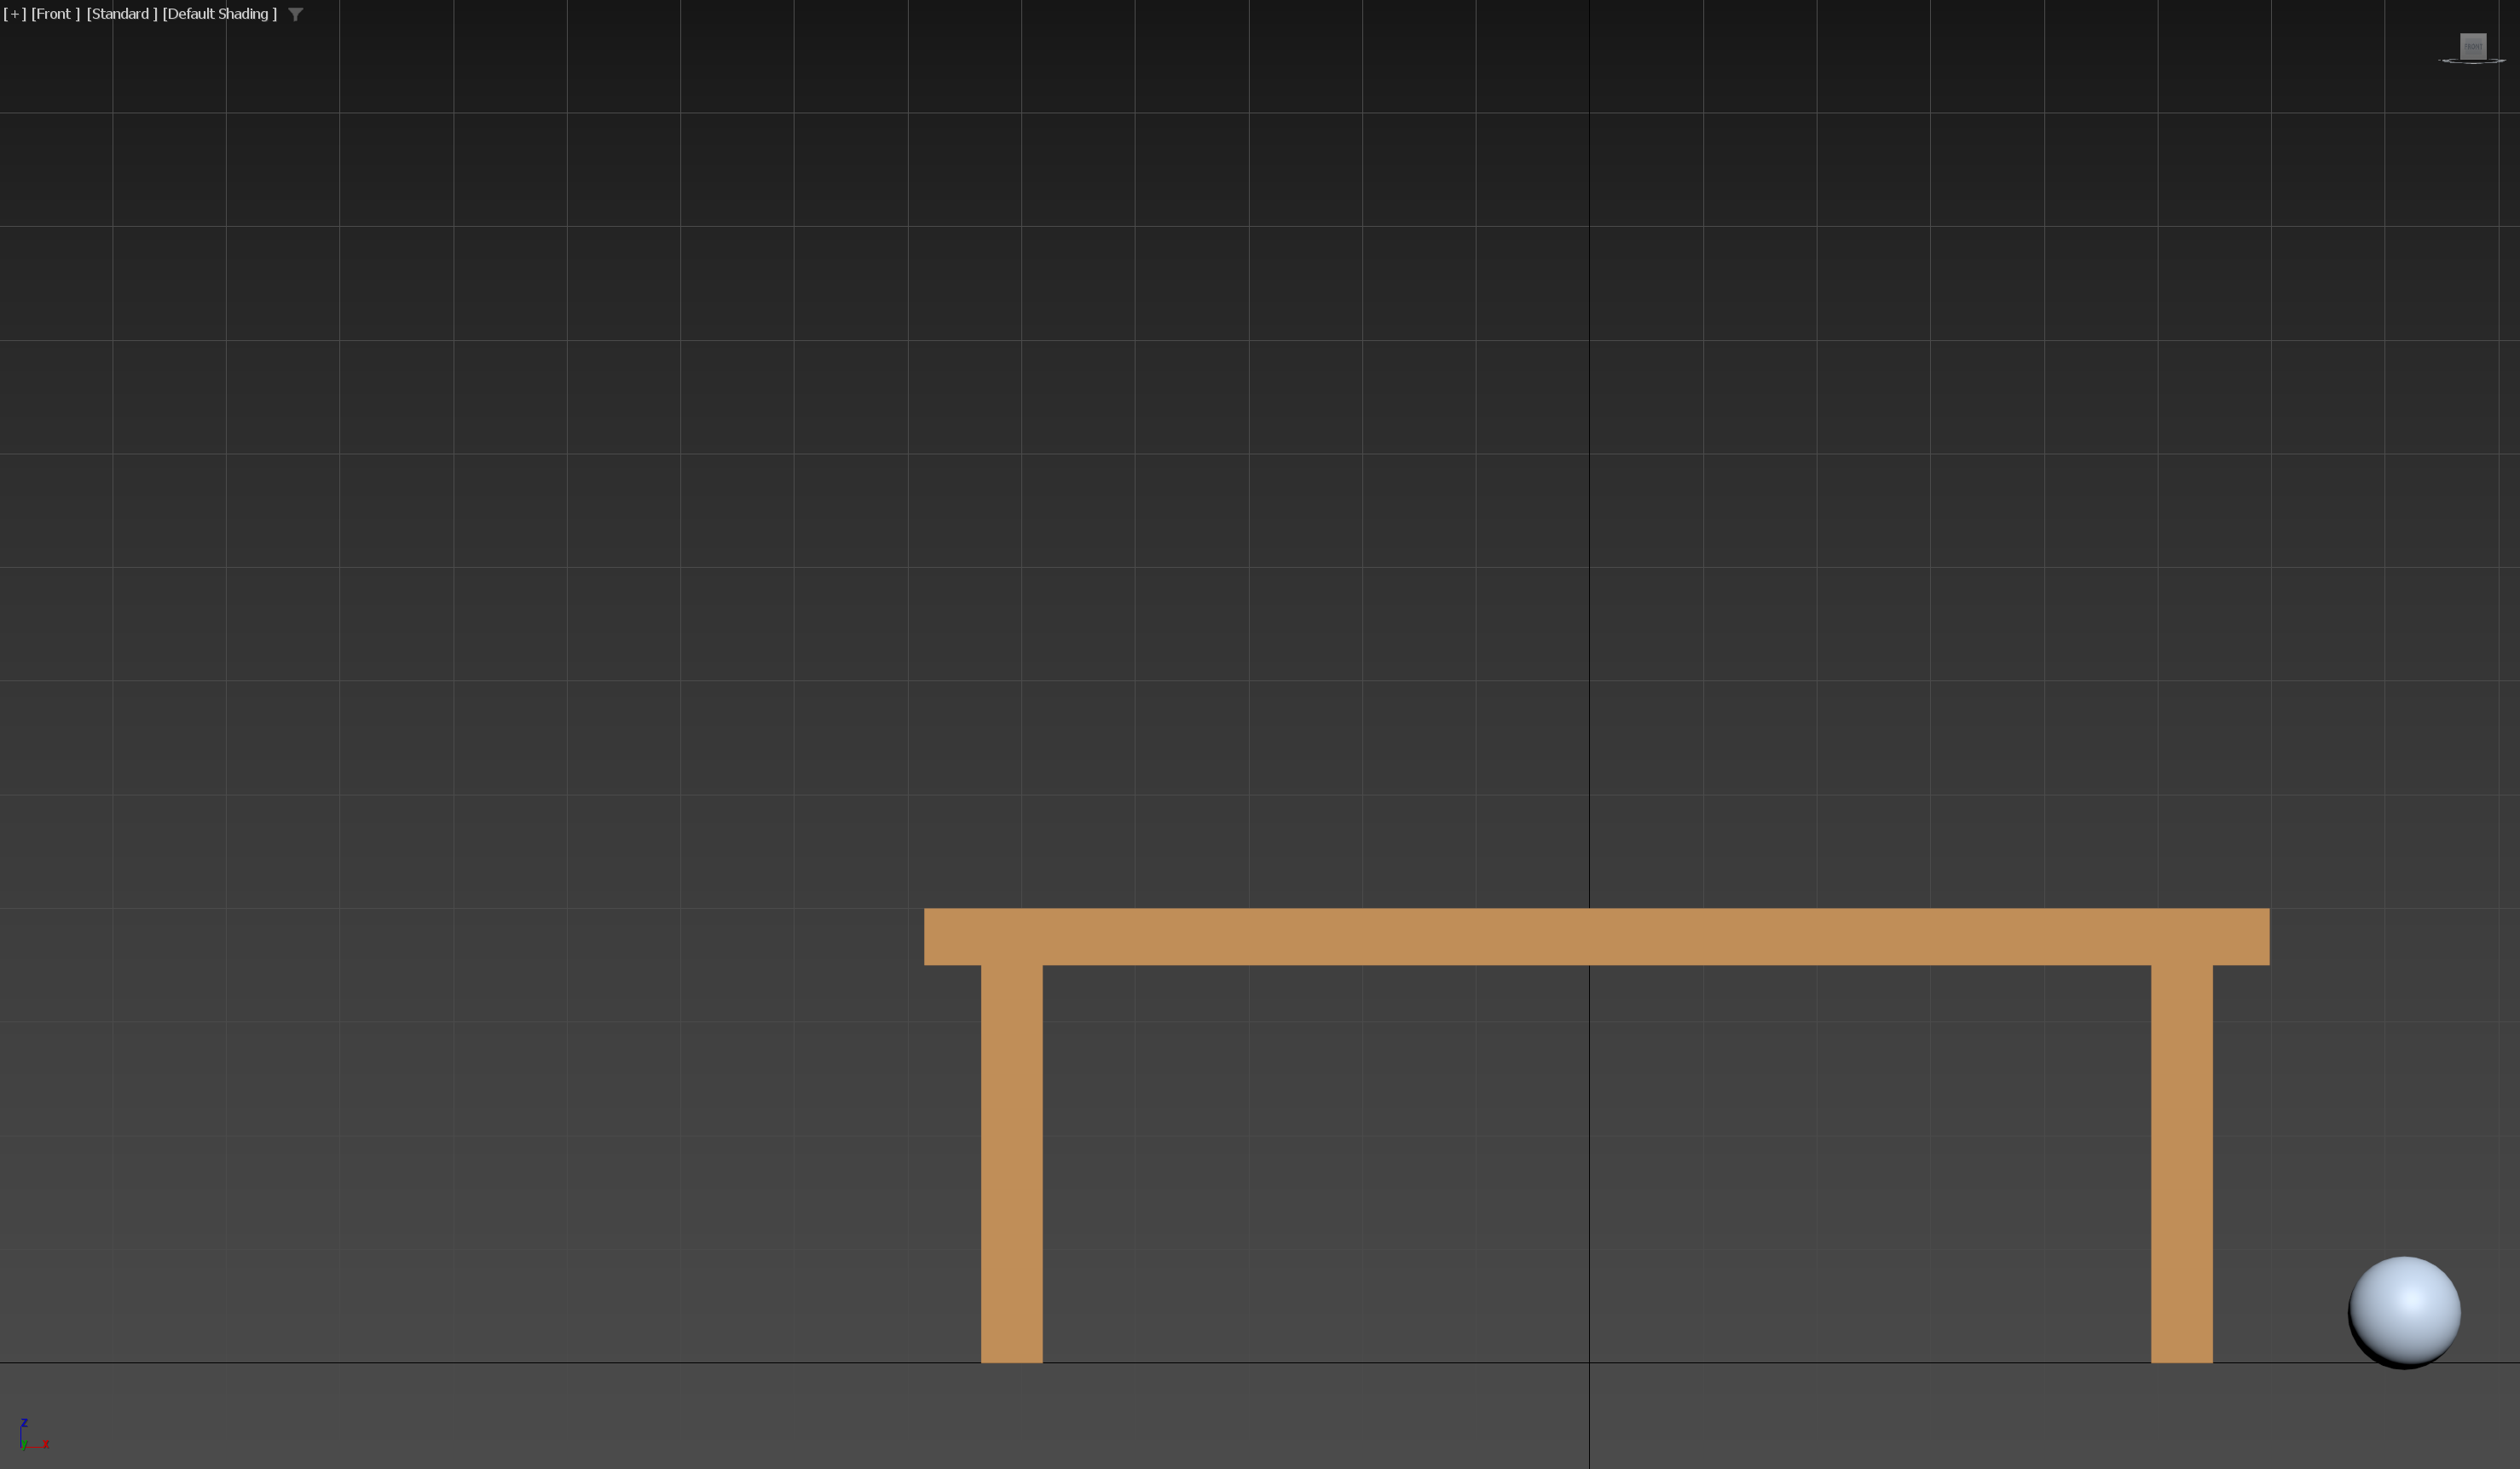
\includegraphics[width=\textwidth]{imagenes/Ejercicio3/keyframes/84.png}
        \caption{Pelota en el instante 84.}
    \end{subfigure}
    \caption{\textit{Keyframes} utilizados para animar la pelota.}
\end{figure}
Y para animar los rebotes y el movimiento de manera realista, se han usado las siguientes curvas en la pelota:

% imagenes separadas de las curvas
\begin{figure}[H]
    \centering
    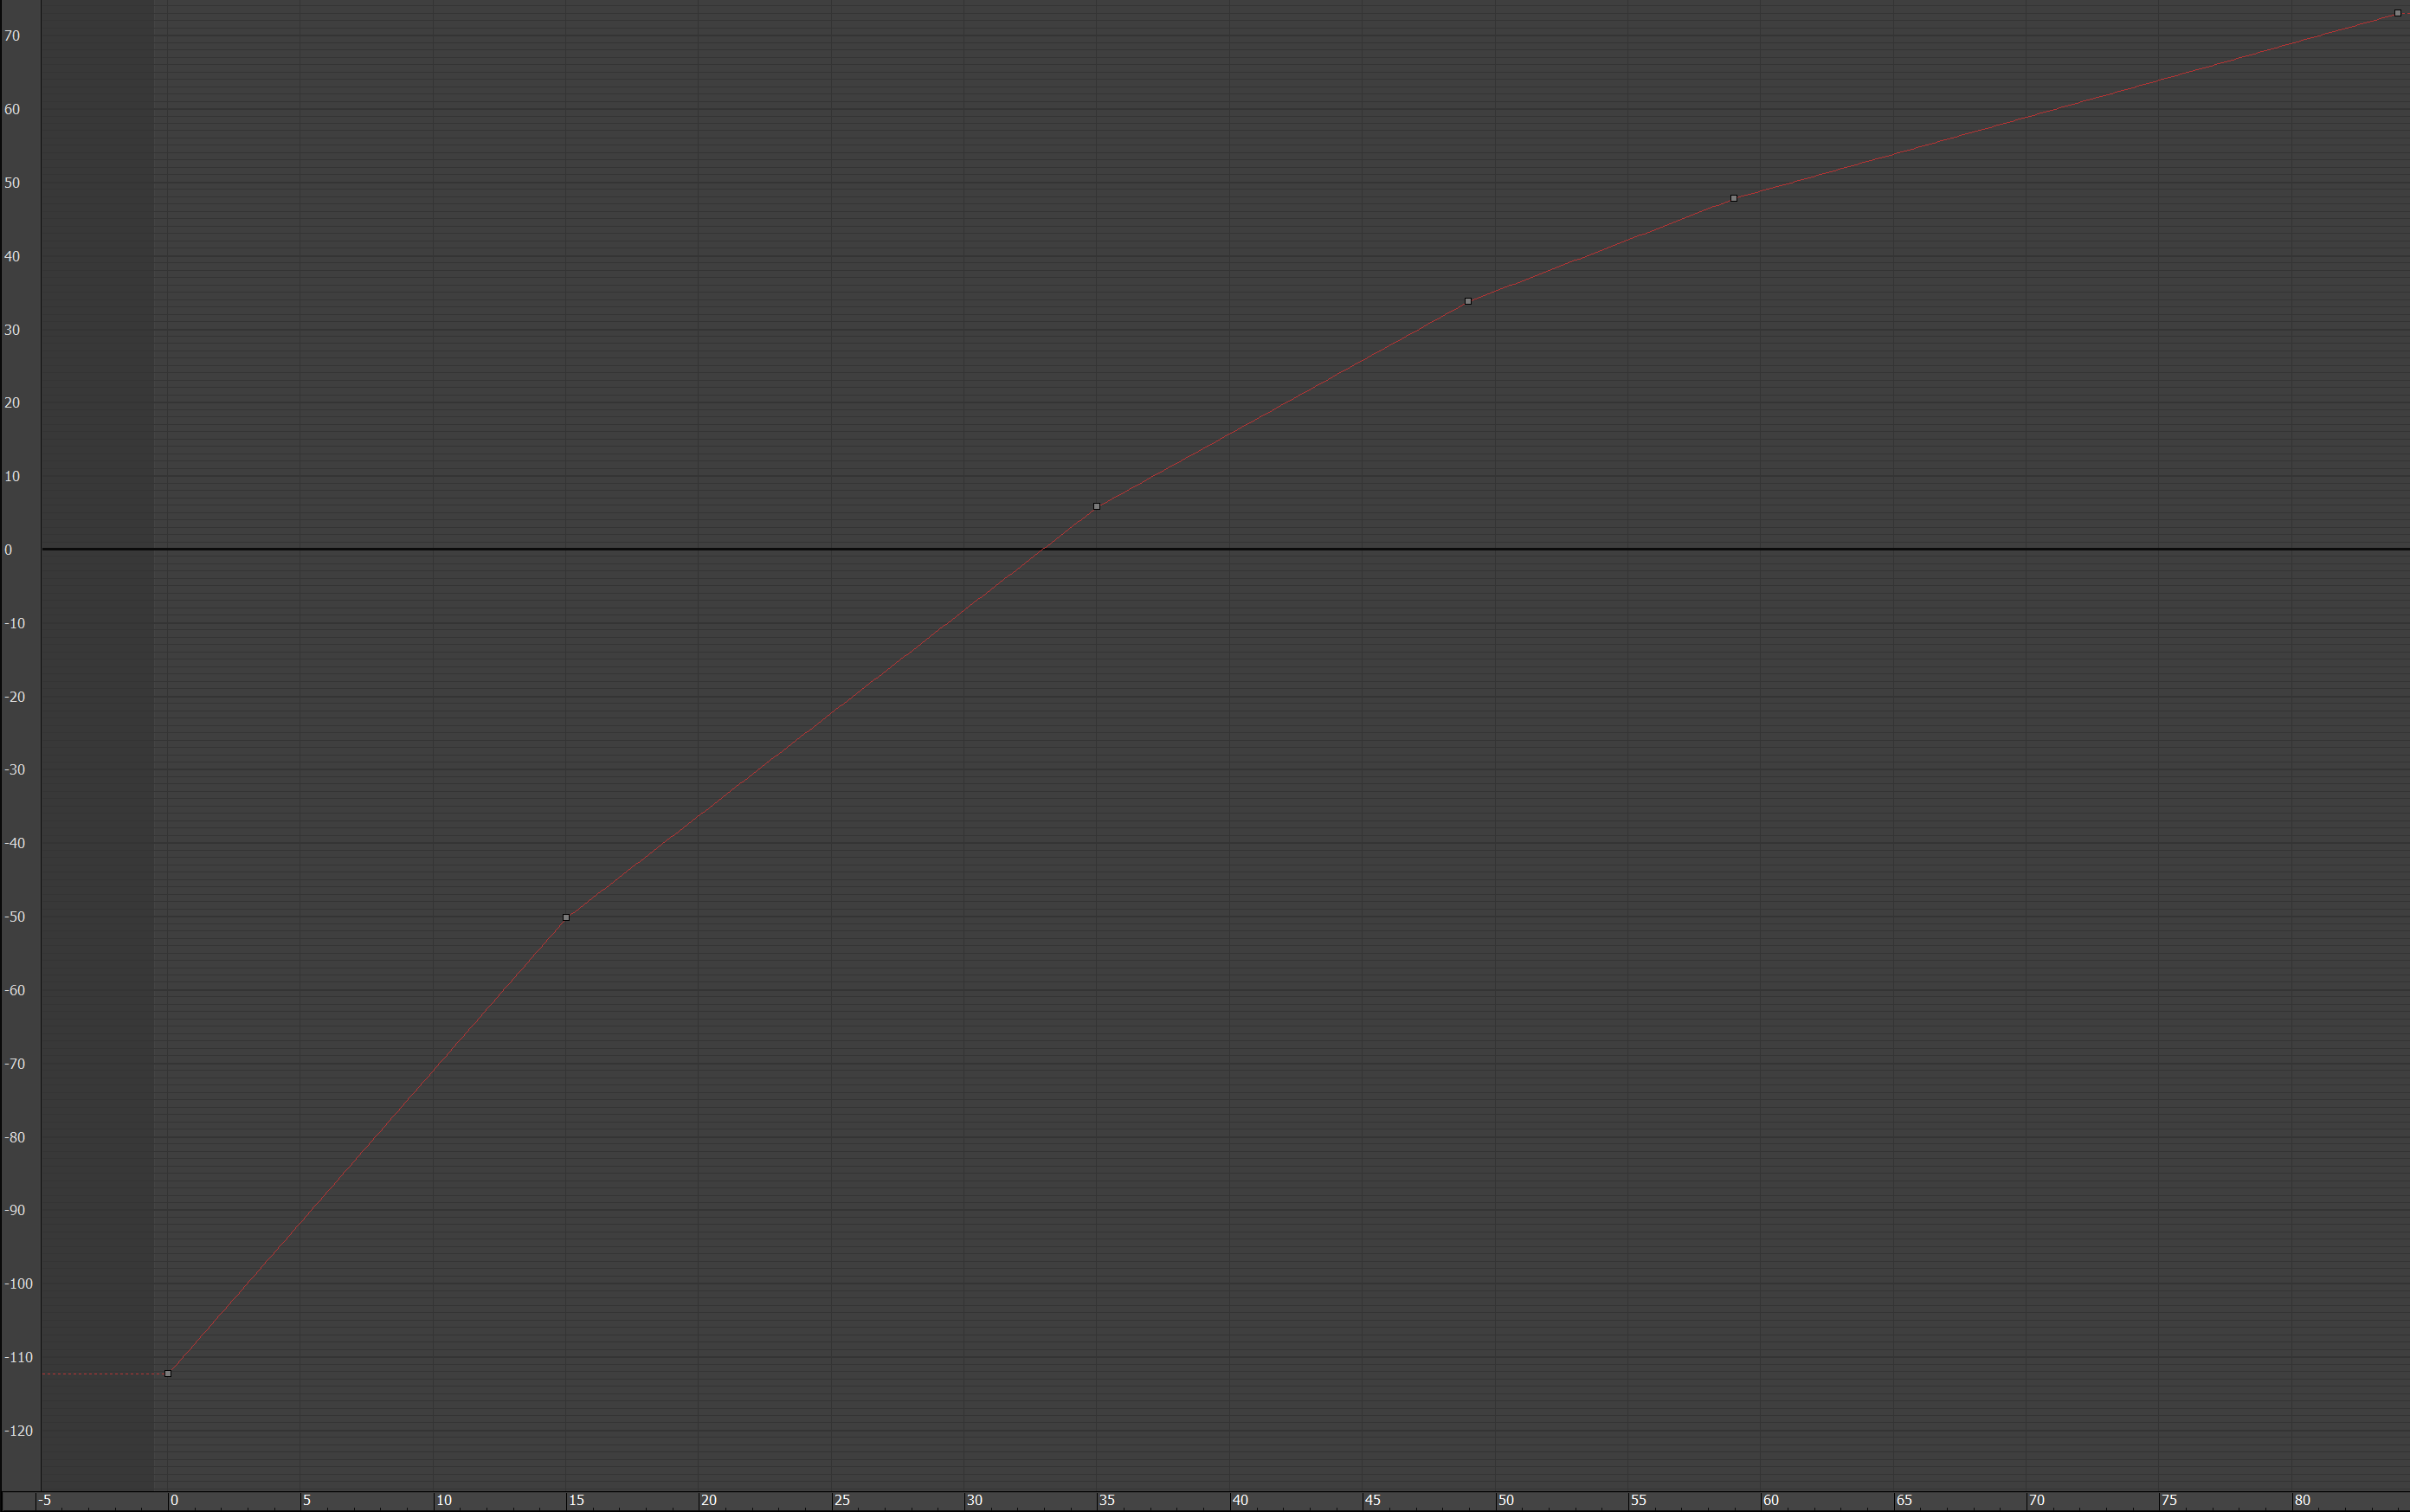
\includegraphics[width=0.8\textwidth]{imagenes/Ejercicio3/corregidas/curvas/red.png}
    \caption{Posición de la pelota en el eje X.}
\end{figure}

La curva de color rojo (Posición en el eje X) sigue una forma lineal para todos los \textit{keyframes}. También se puede observar como el conjunto de todos los \textit{keyframes}, al seguir el factor 2, tiene una forma exponencial, haciendo que en la animación la pelota vaya recorriendo cada vez menos distancia para la misma cantidad de tiempo.

\bigskip

Un aspecto importante a tener en cuenta es que esta curva se podría haber hecho con menos \textit{keyframes}, pero para darle más realismo he decidido implementar un factor de 2, al igual que en la altura. Por lo que realmente todos los \textit{keyframes} que aparecen son necesarios.

\newpage

Además, he eliminado los \textit{keyframes} relativos a cuando la pelota estaba en el aire, ya que no tenían ningún sentido. Esto se puede ver en la siguiente imagen:

\begin{figure}[H]
    \centering
    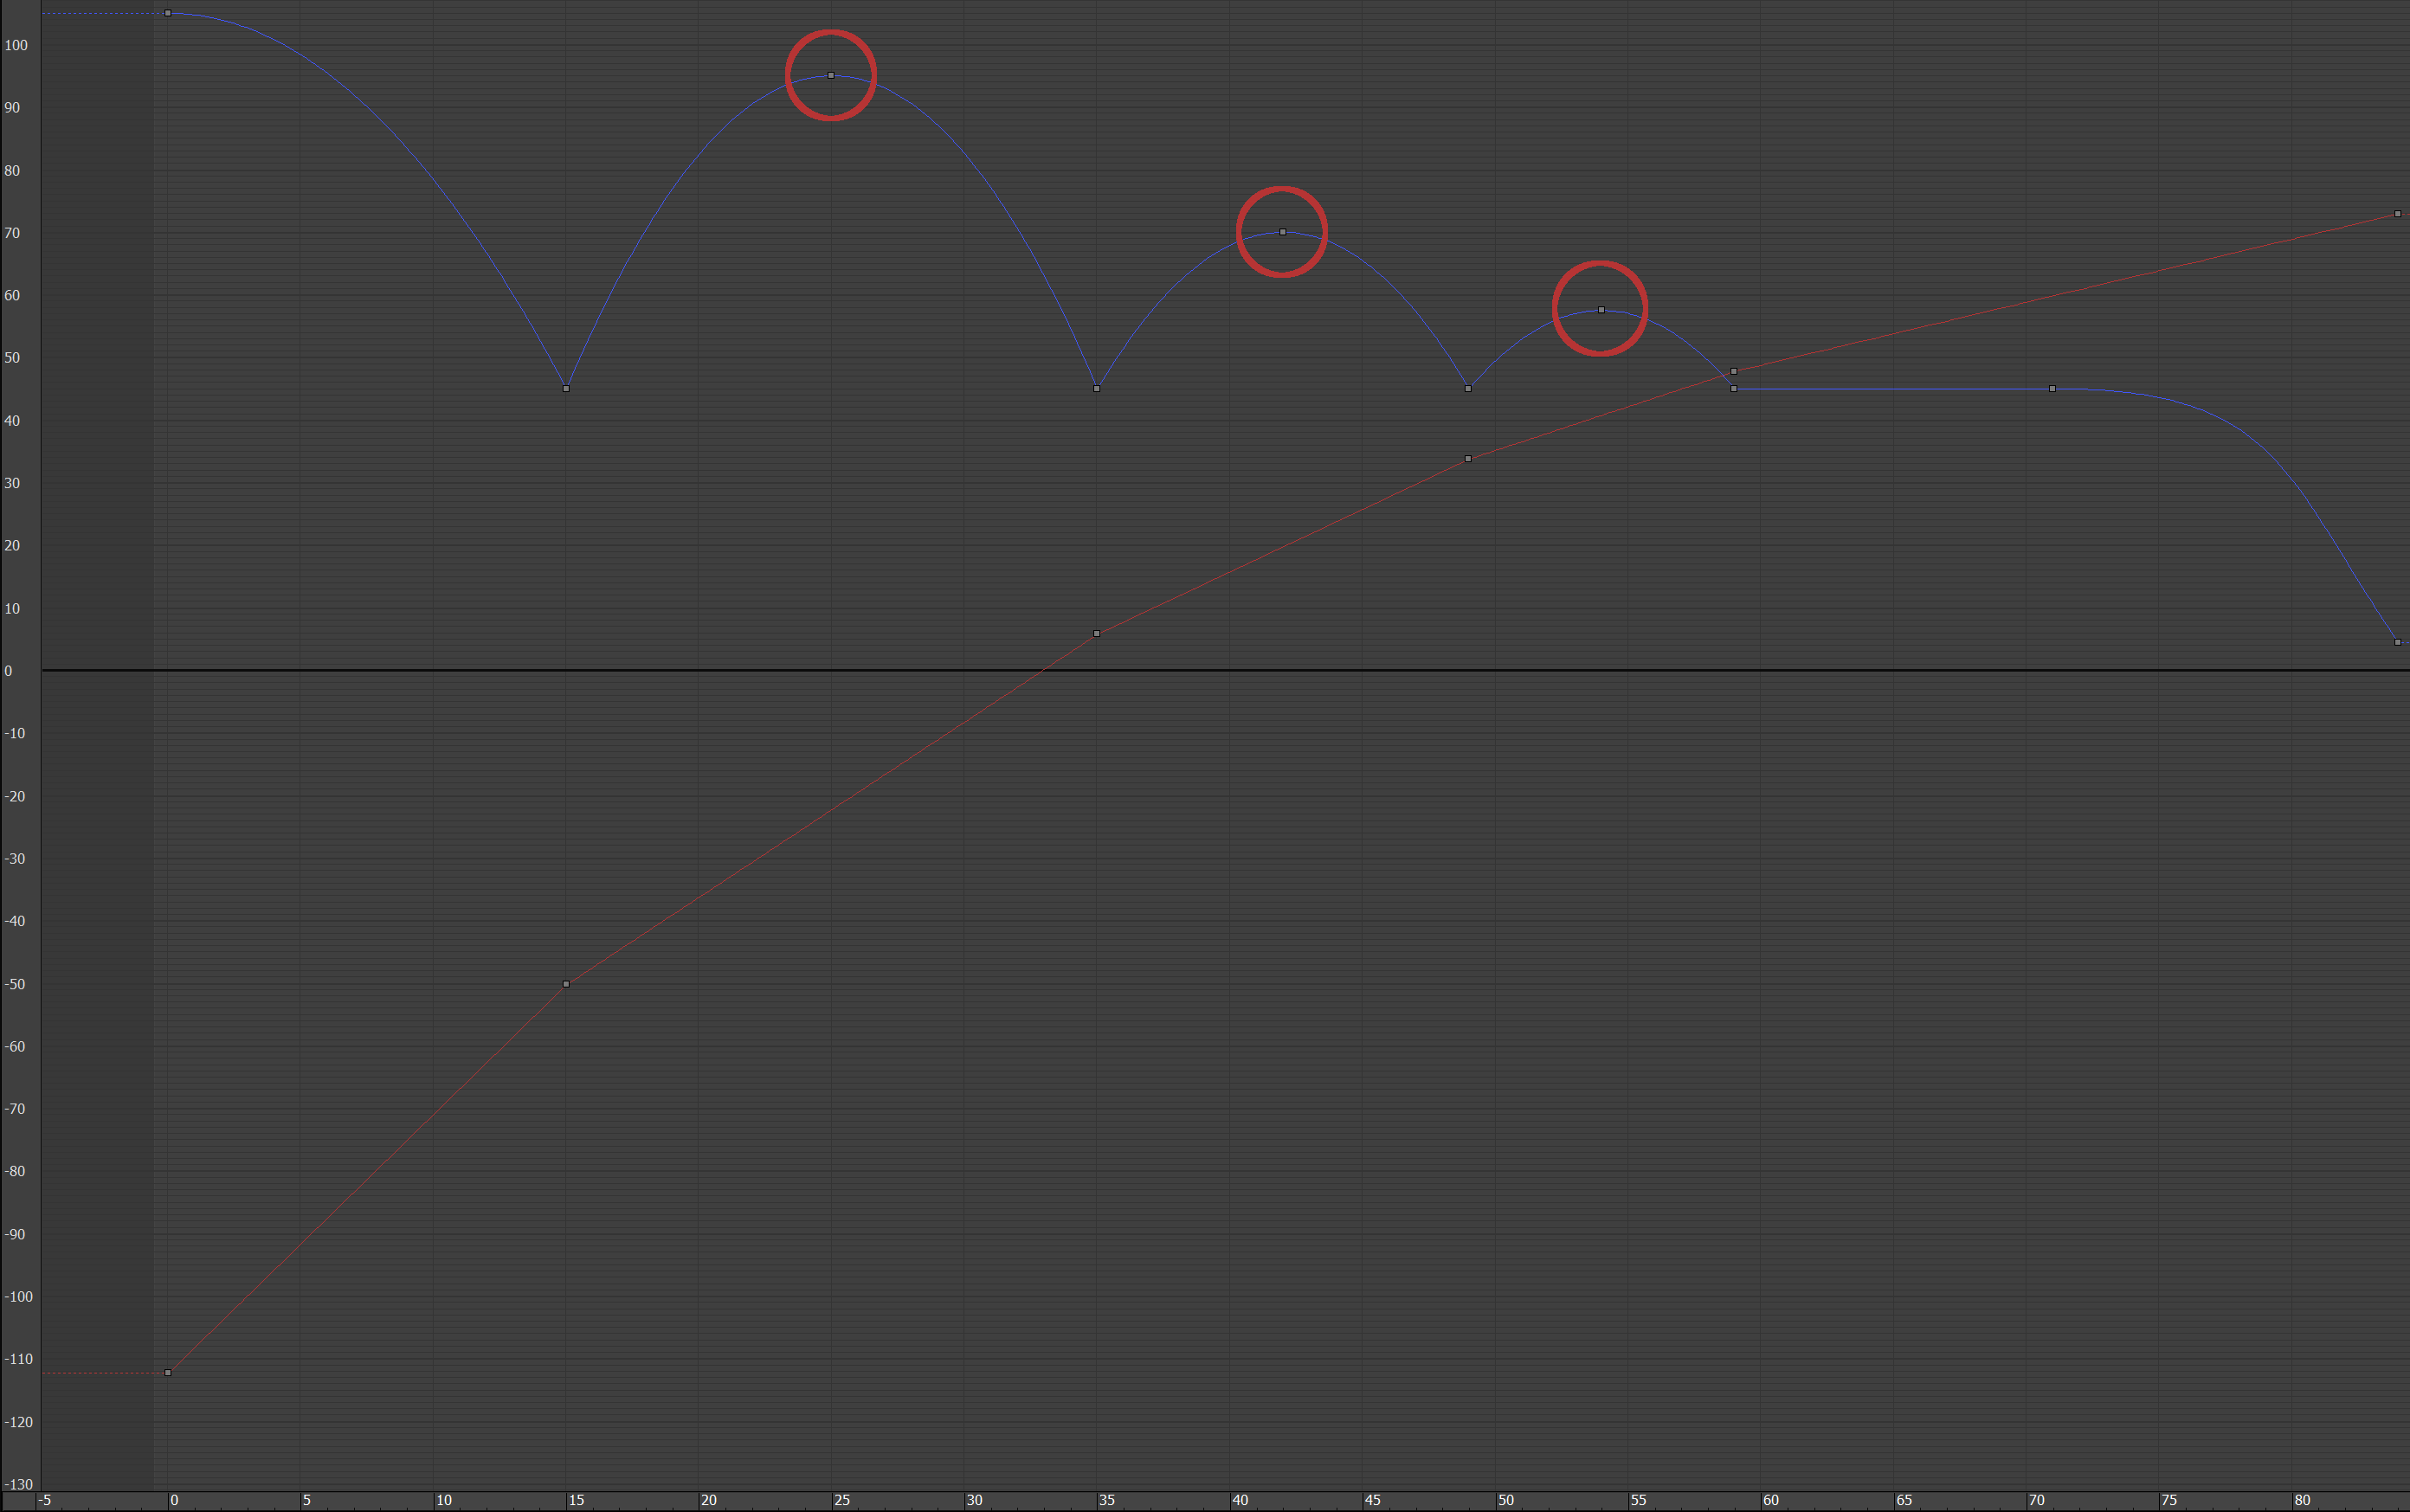
\includegraphics[width=0.8\textwidth]{imagenes/Ejercicio3/corregidas/curvas/both.png}
    \caption{Se puede apreciar como la curva roja no tiene \textit{keyframes} en los instantes rodeados en rojo.}
\end{figure}

\begin{figure}[H]
    \centering
    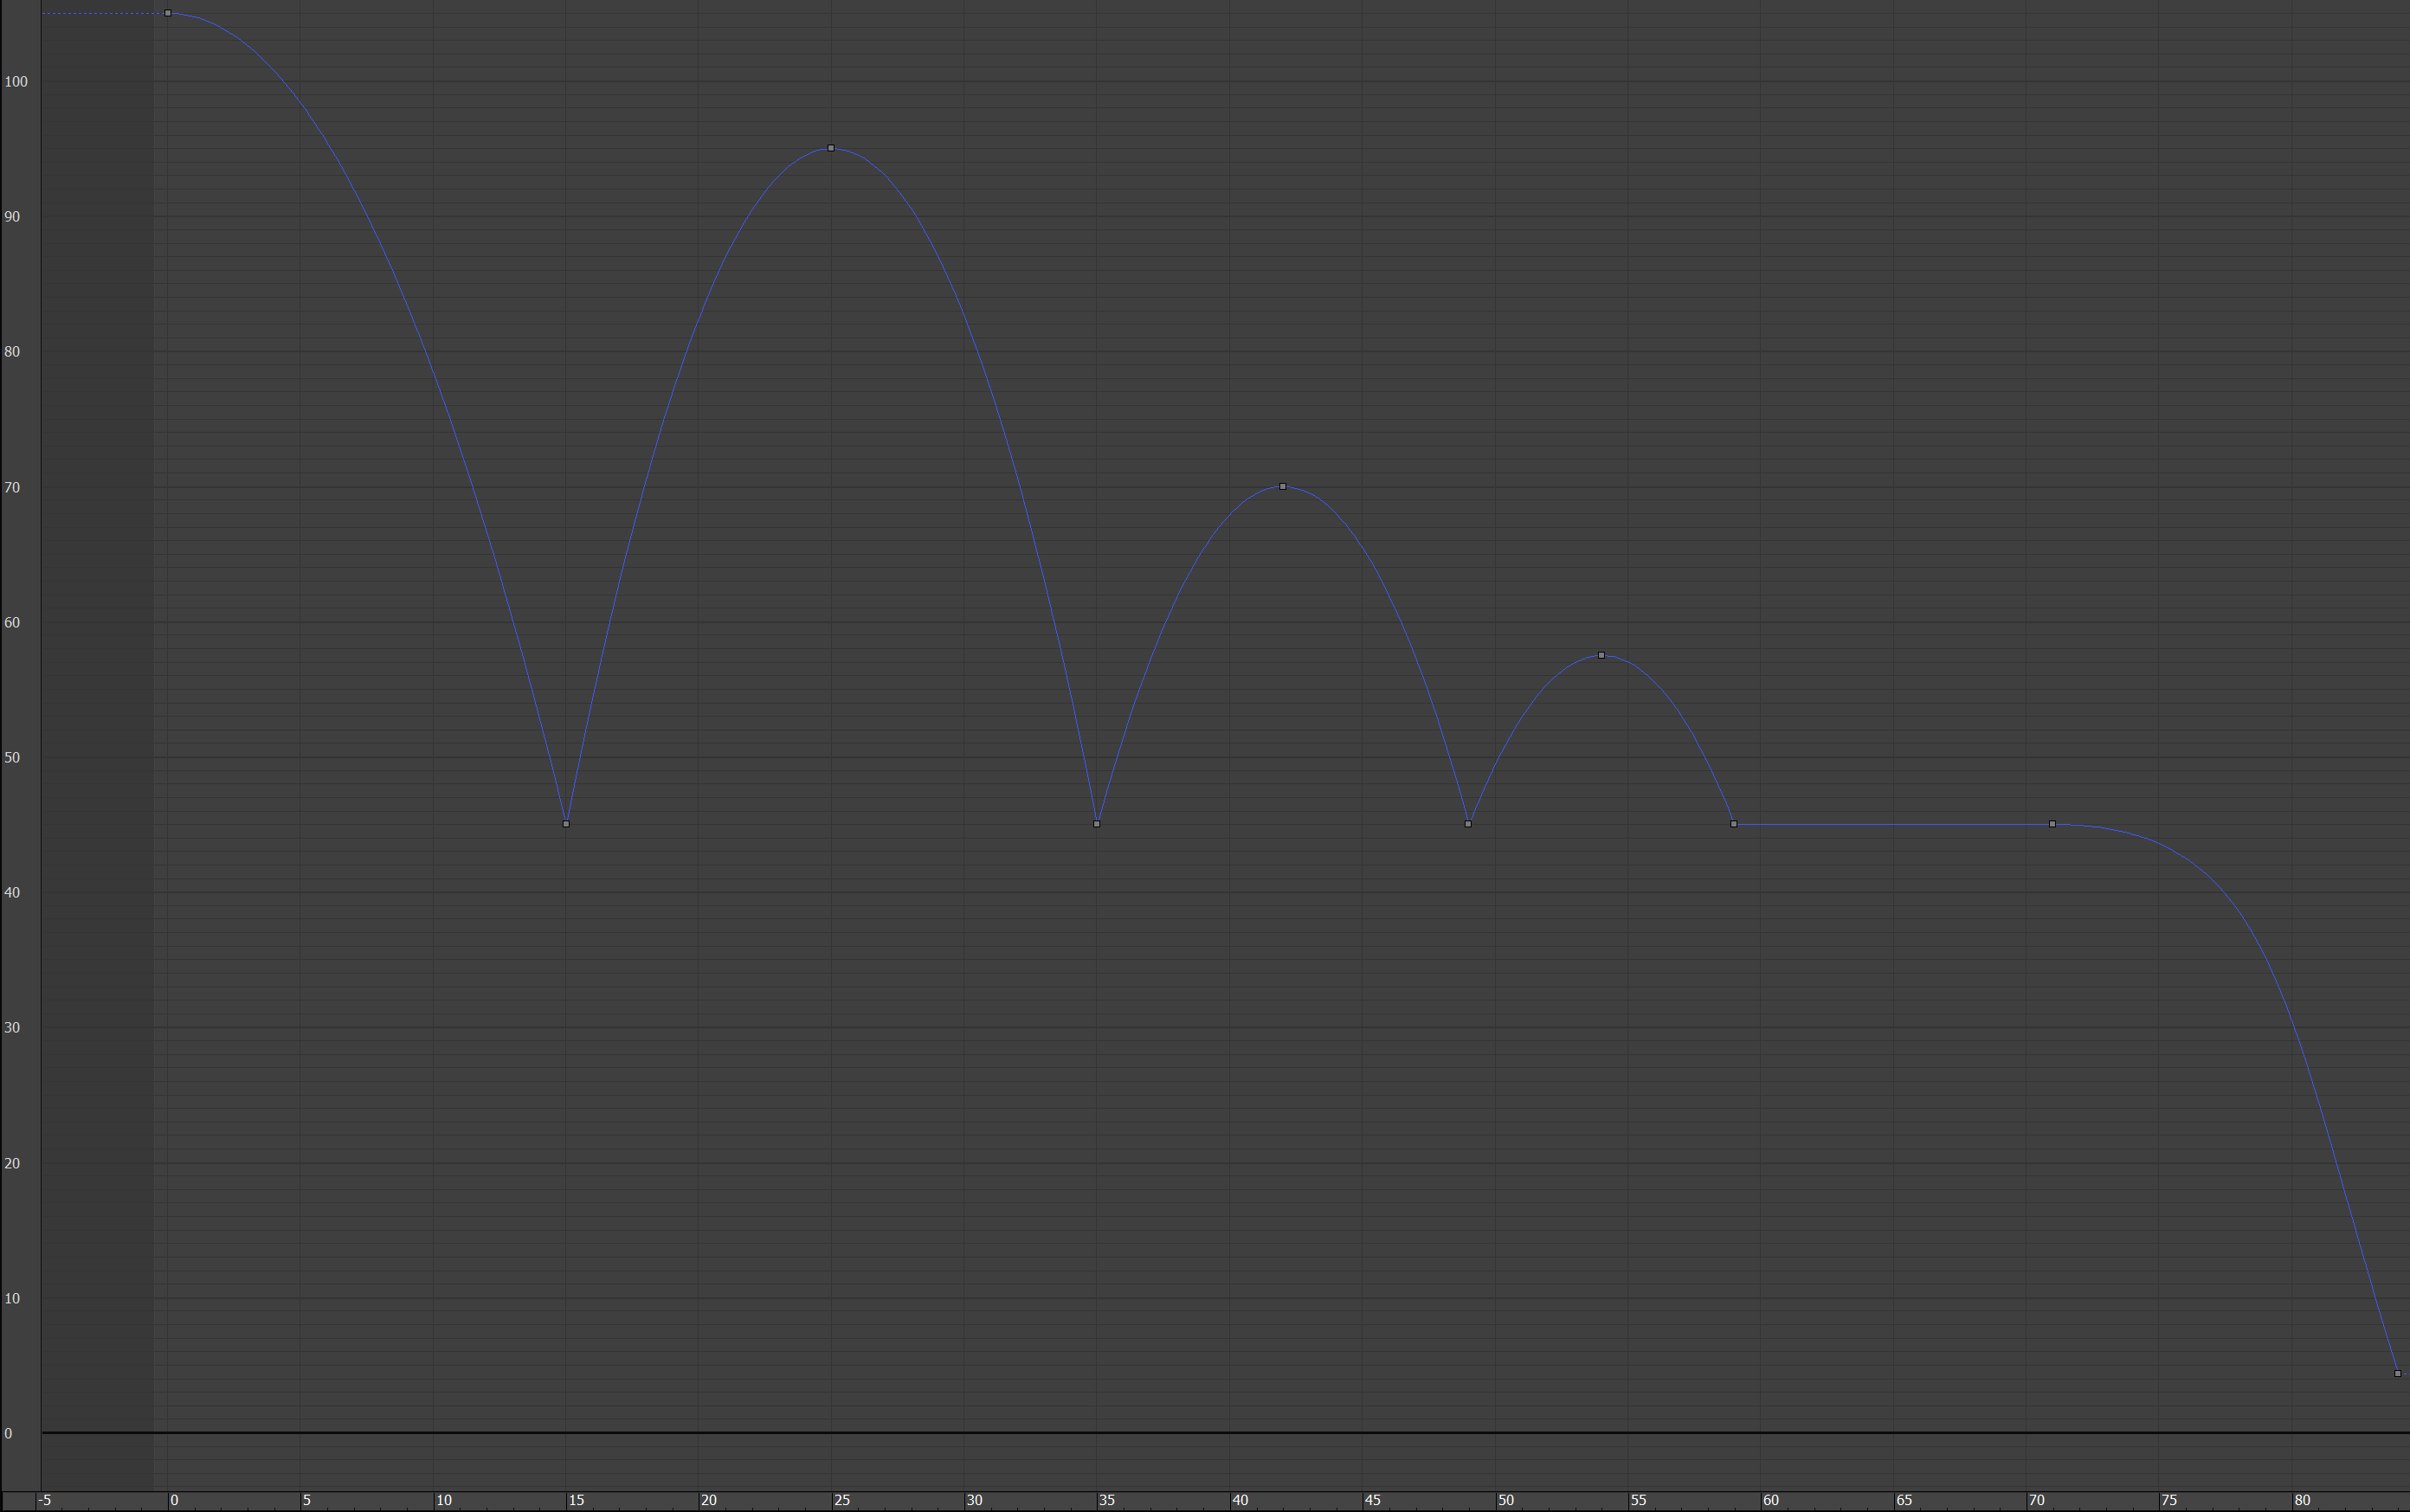
\includegraphics[width=0.8\textwidth]{imagenes/Ejercicio3/corregidas/curvas/blue.png}
    \caption{Posición de la pelota en el eje Z.}
\end{figure}

La curva de color azul (Posición en el eje Z) sigue las trayectorias que hace la bola. Para que los rebotes sean realistas, he utilizado una curva de desaceleración en la subida y otro de aceleración en la bajada, para simular el efecto de la gravedad en la pelota. Cuando cae de la mesa se sigue la misma curva de aceleración anteriormente mencionada.

\newpage

\section{Ejercicio 4 - Montacargas}

En este ejercicio se pide animar un montacargas que se desplaza desde la izquierda hasta la derecha y se detiene bruscamente al final, aplicando el principio de \textit{Overlap \& Follow Through}. Por tanto, la cadena del montacargas debe ser ``arrastrada'' por la plataforma y, cuando esta pare, la cadena debe dar un latigazo en el sentido contrario antes de detenerse en su lugar final.

\bigskip

Para crear la figura del montacargas se ha utilizado un cubo achatado como plataforma y para la cadena se ha empleado un cilindro y una esfera para la articulación. Con estas dos figuras, se han anidado las distintas secciones de la cadena, de modo que el segmento inferior es el hijo y el superior el padre, logrando así que el hijo herede las transformaciones del padre.

%foto de la jerarquia
\begin{figure}[H]
    \centering
    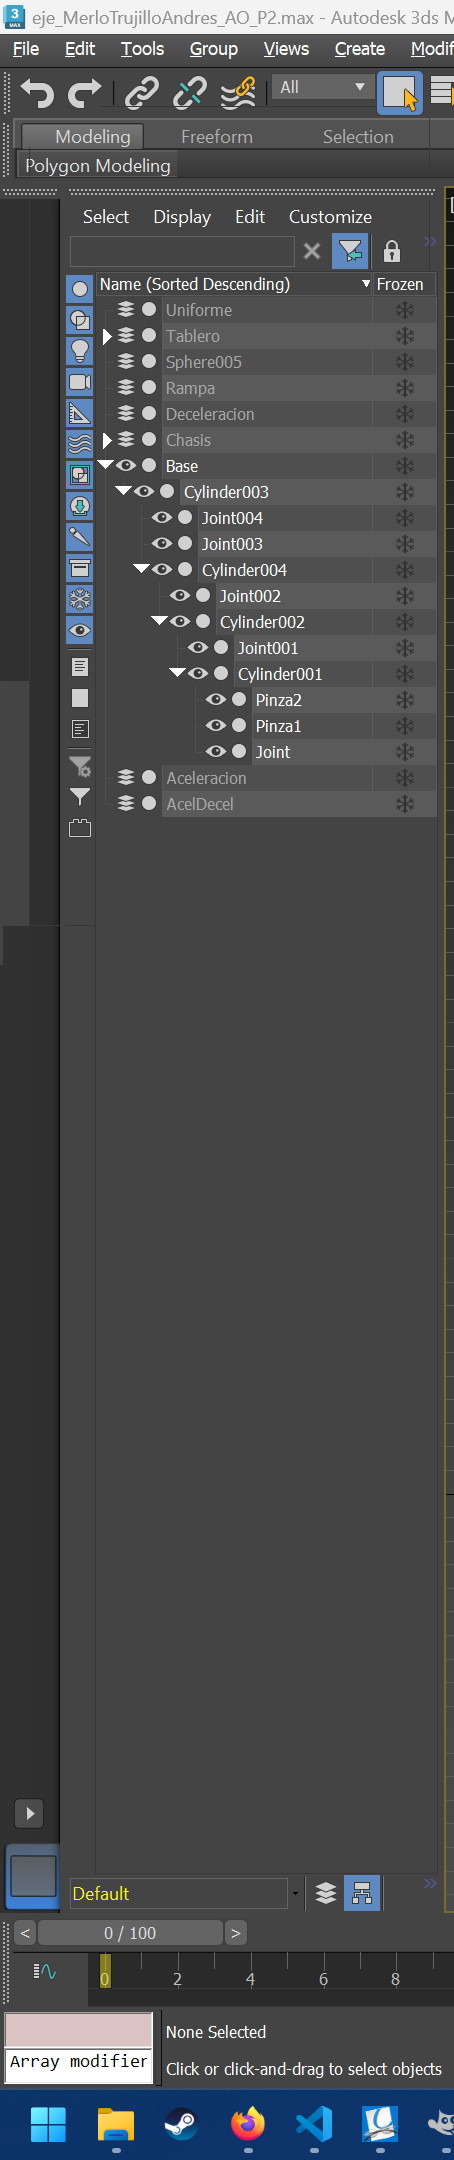
\includegraphics[width=0.5\textwidth]{imagenes/Ejercicio4/jerarquia.png}
    \caption{Jerarquía de las distintas partes del montacargas.}
\end{figure}

En cuanto a la animación, ha sido necesario utilizar 2 \textit{keyframes} para la plataforma y 7 \textit{keyframes} para cada una de las partes de la cadena, pero estas realizan la misma animación.

\bigskip

\textit{Keyframes} de la plataforma:

\begin{enumerate}
    \item \textbf{Instante 0:} Posición inicial, a la izquierda del todo.
    \item \textbf{Instante 30:} Posición final, a la derecha del todo.
\end{enumerate}

\bigskip

\textit{Keyframes} generales de la cadena:

\begin{enumerate}
    \item \textbf{Instante 0:} Se encuentra el segmento en reposo; es decir, en vertical.
    \item \textbf{Instante 18:} Se encuentra cada segmento de la cadena rotado al máximo, siendo arrastrado por la plataforma en movimiento.
    \item \textbf{Instante 30:} Exactamente igual que antes, pero en este caso la plataforma ya ha parado.
    \item \textbf{Instante 47:} Cada segmento de la cadena ahora se encuentra rotado al lado contrario, como resultado de la parada brusca de la plataforma, lo que provoca un latigazo en la cadena.
    \item \textbf{Instante 64:} Cada segmento vuelve a estar rotado hacia el otro lado, pero esta vez con una rotación algo menor que la primera vez, simulando las distintas fuerzas que actúan.
    \item \textbf{Instante 80:} Los segmentos vuelven a estar rotados al lado contrario, pero con una cantidad de rotación mucho menor, casi vertical.
    \item \textbf{Instante 96:} Los segmentos se encuentran de nuevo verticales, como en el instante 0.
\end{enumerate}
%keyframes
\bigskip

A modo visual, los \textit{keyframes} son los siguientes:
\begin{figure}[H]
    \centering
    \begin{subfigure}[H]{0.48\textwidth}
        \centering
        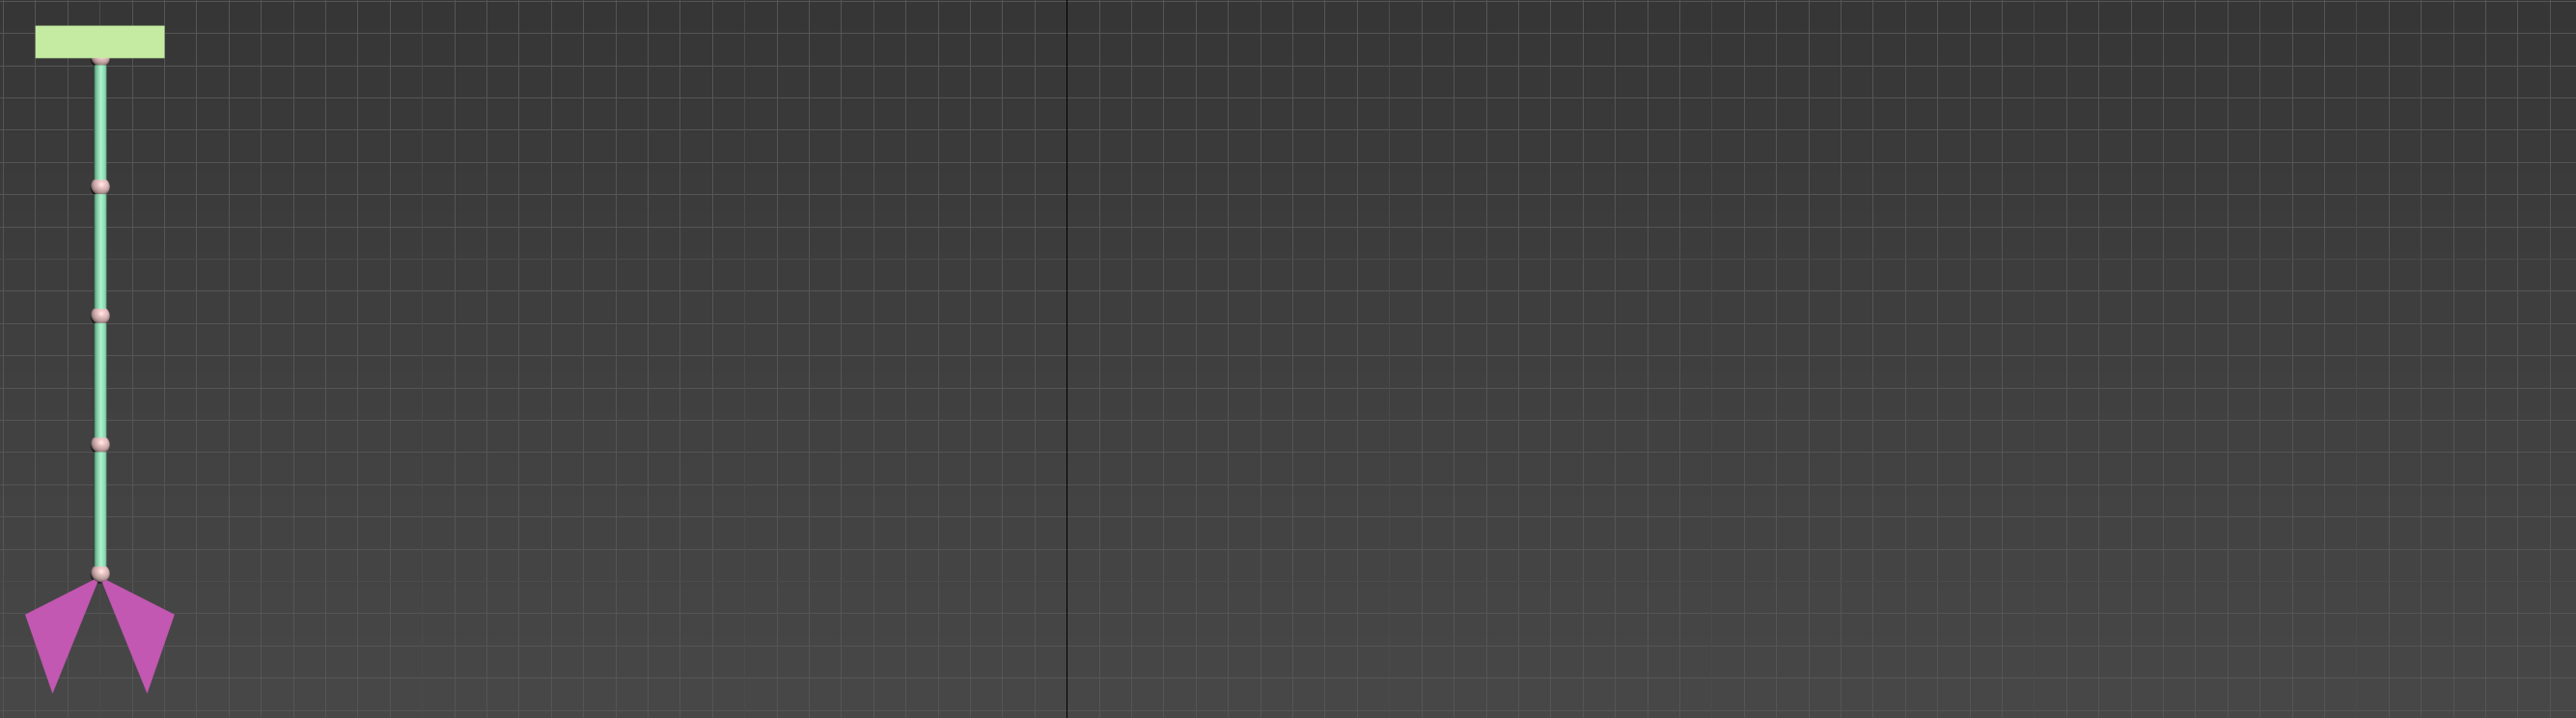
\includegraphics[width=\textwidth]{imagenes/Ejercicio4/keyframes/0.png}
        \caption{Rotación de los segmentos de la cadena en el instante 0. También es el \textit{keyframe} de la plataforma.}
    \end{subfigure}
    \hfill
    \begin{subfigure}[H]{0.48\textwidth}
        \centering
        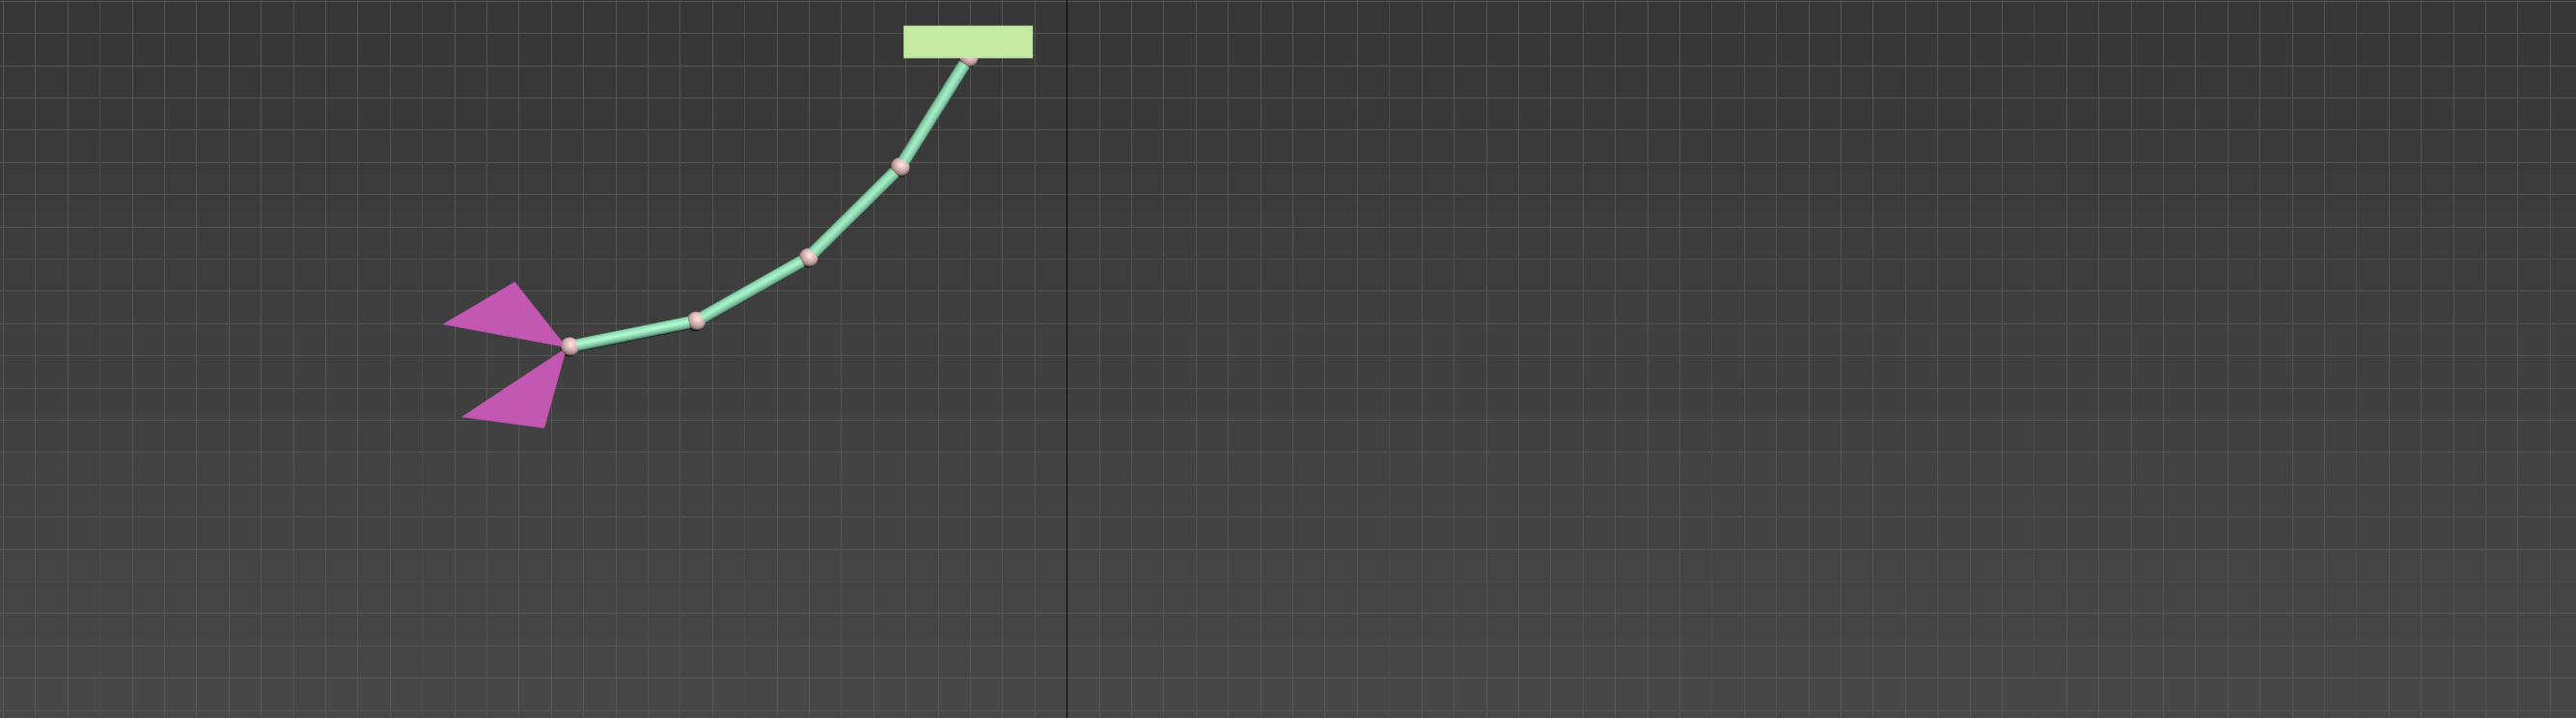
\includegraphics[width=\textwidth]{imagenes/Ejercicio4/keyframes/18.png}
        \caption{Rotación de los segmentos de la cadena en el instante 18.}
    \end{subfigure}
    \par\bigskip
    \begin{subfigure}[H]{0.48\textwidth}
        \centering
        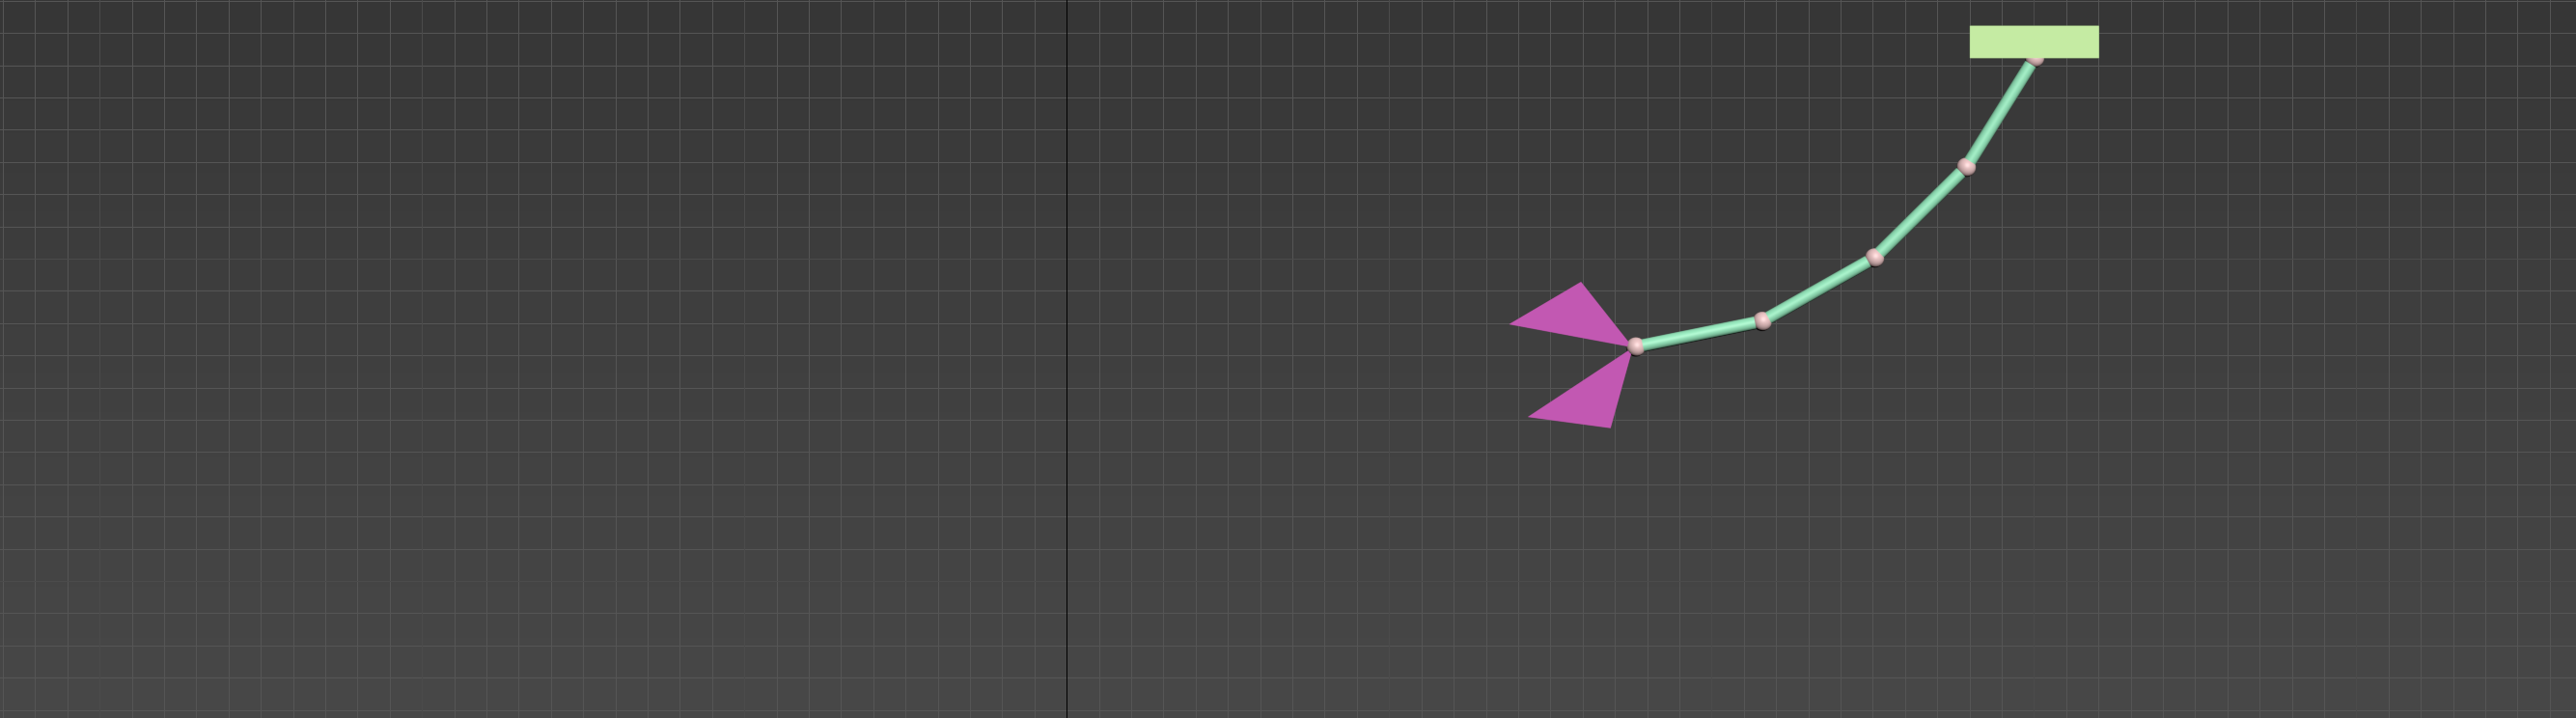
\includegraphics[width=\textwidth]{imagenes/Ejercicio4/keyframes/30.png}
        \caption{Rotación de los segmentos de la cadena en el instante 30. También es el \textit{keyframe} de la plataforma.}
    \end{subfigure}
    \hfill
    \begin{subfigure}[H]{0.48\textwidth}
        \centering
        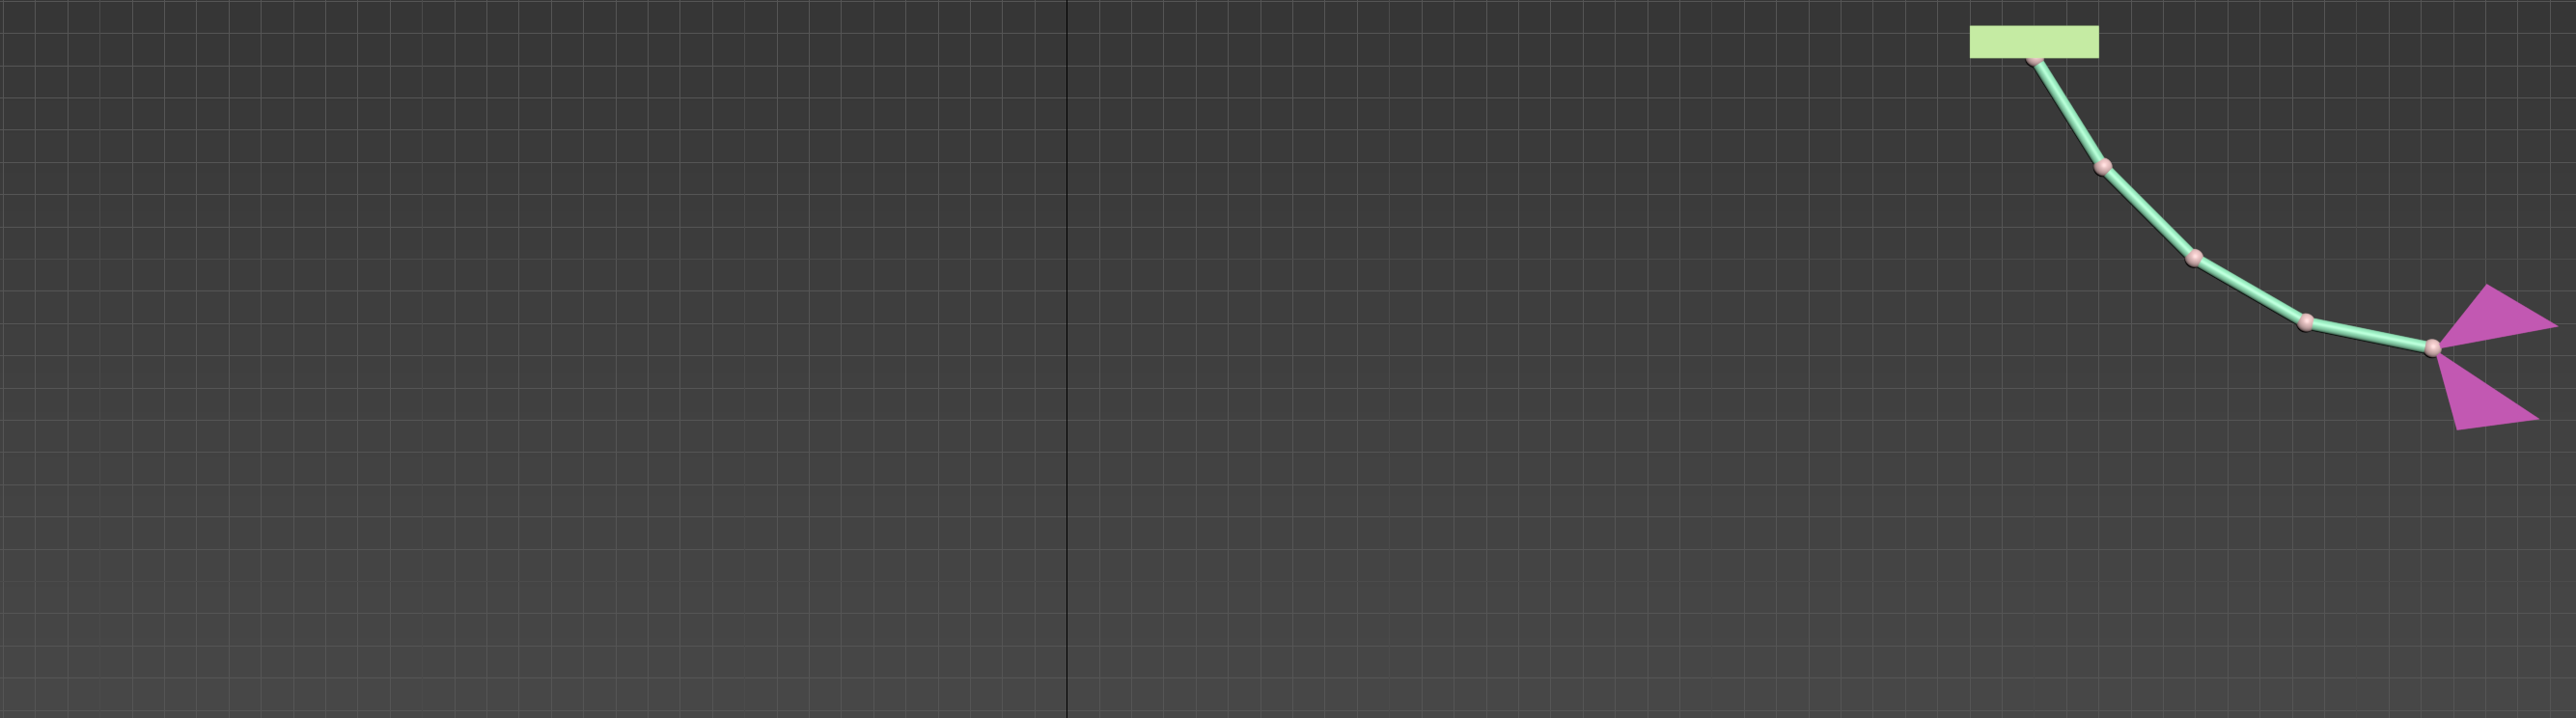
\includegraphics[width=\textwidth]{imagenes/Ejercicio4/keyframes/47.png}
        \caption{Rotación de los segmentos de la cadena en el instante 47.}
    \end{subfigure}
    \par\bigskip
    \begin{subfigure}[H]{0.48\textwidth}
        \centering
        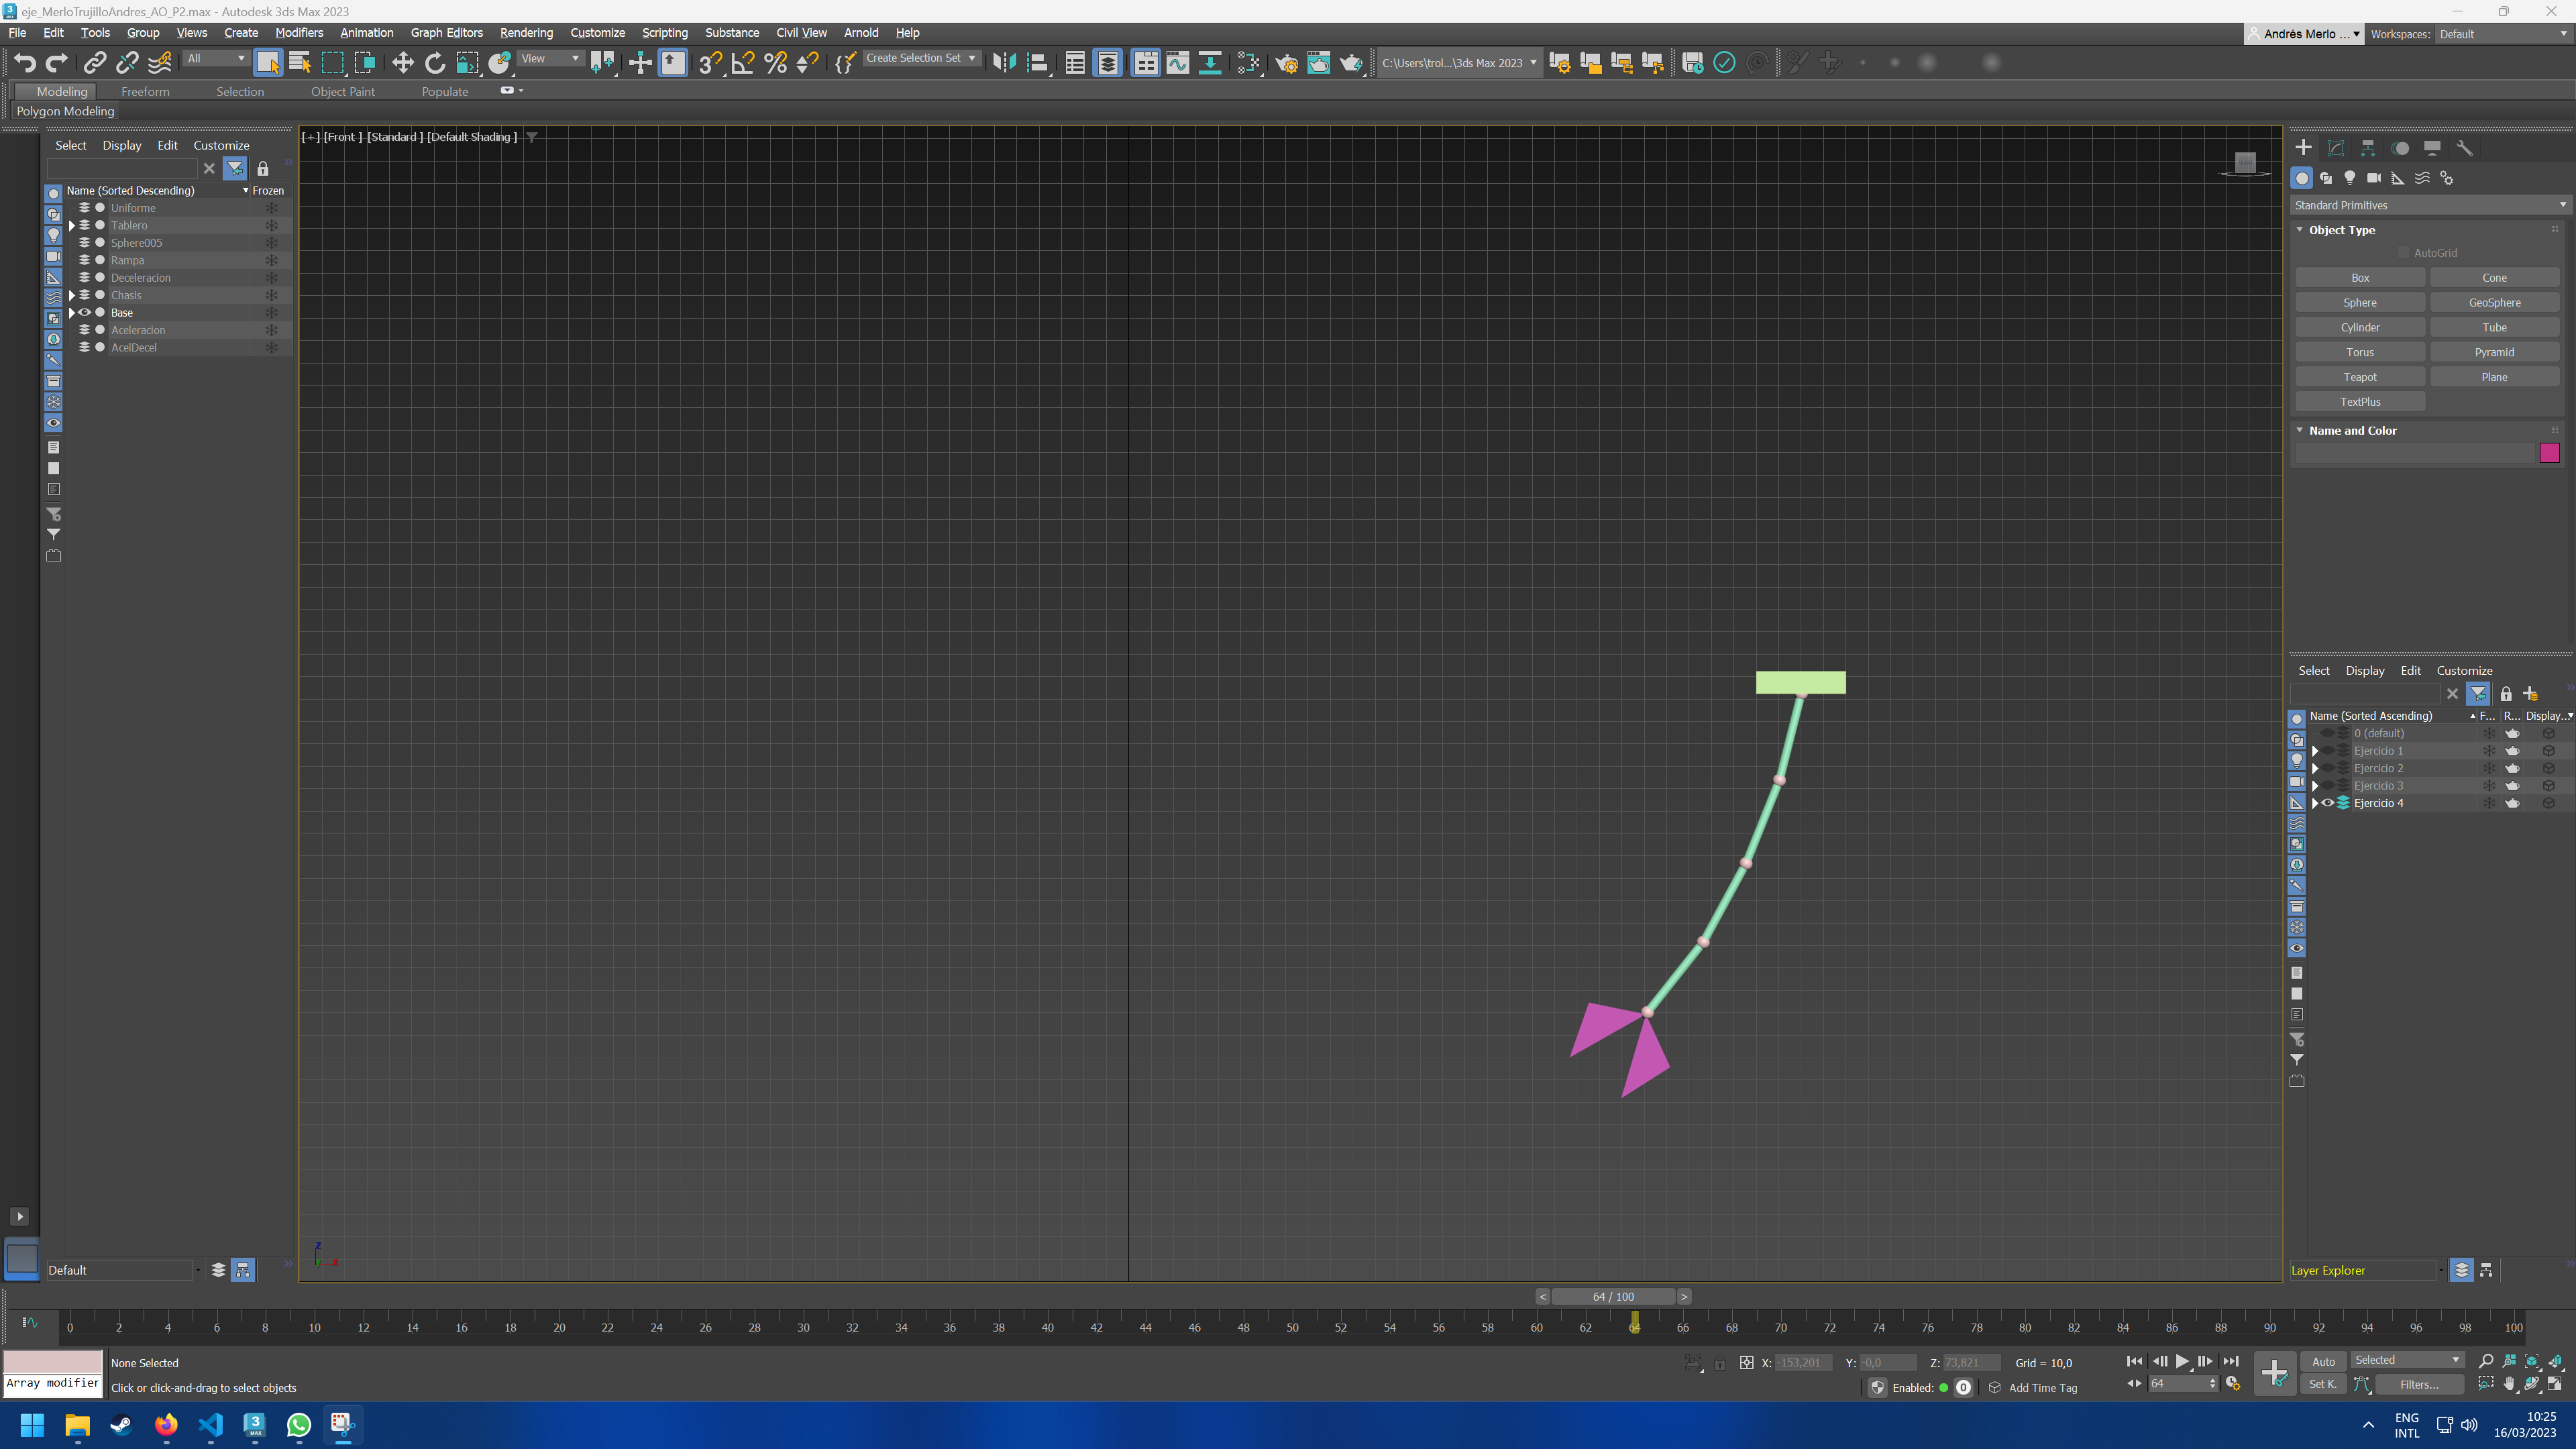
\includegraphics[width=\textwidth]{imagenes/Ejercicio4/keyframes/64.png}
        \caption{Rotación de los segmentos de la cadena en el instante 64.}
    \end{subfigure}
    \hfill
    \begin{subfigure}[H]{0.48\textwidth}
        \centering
        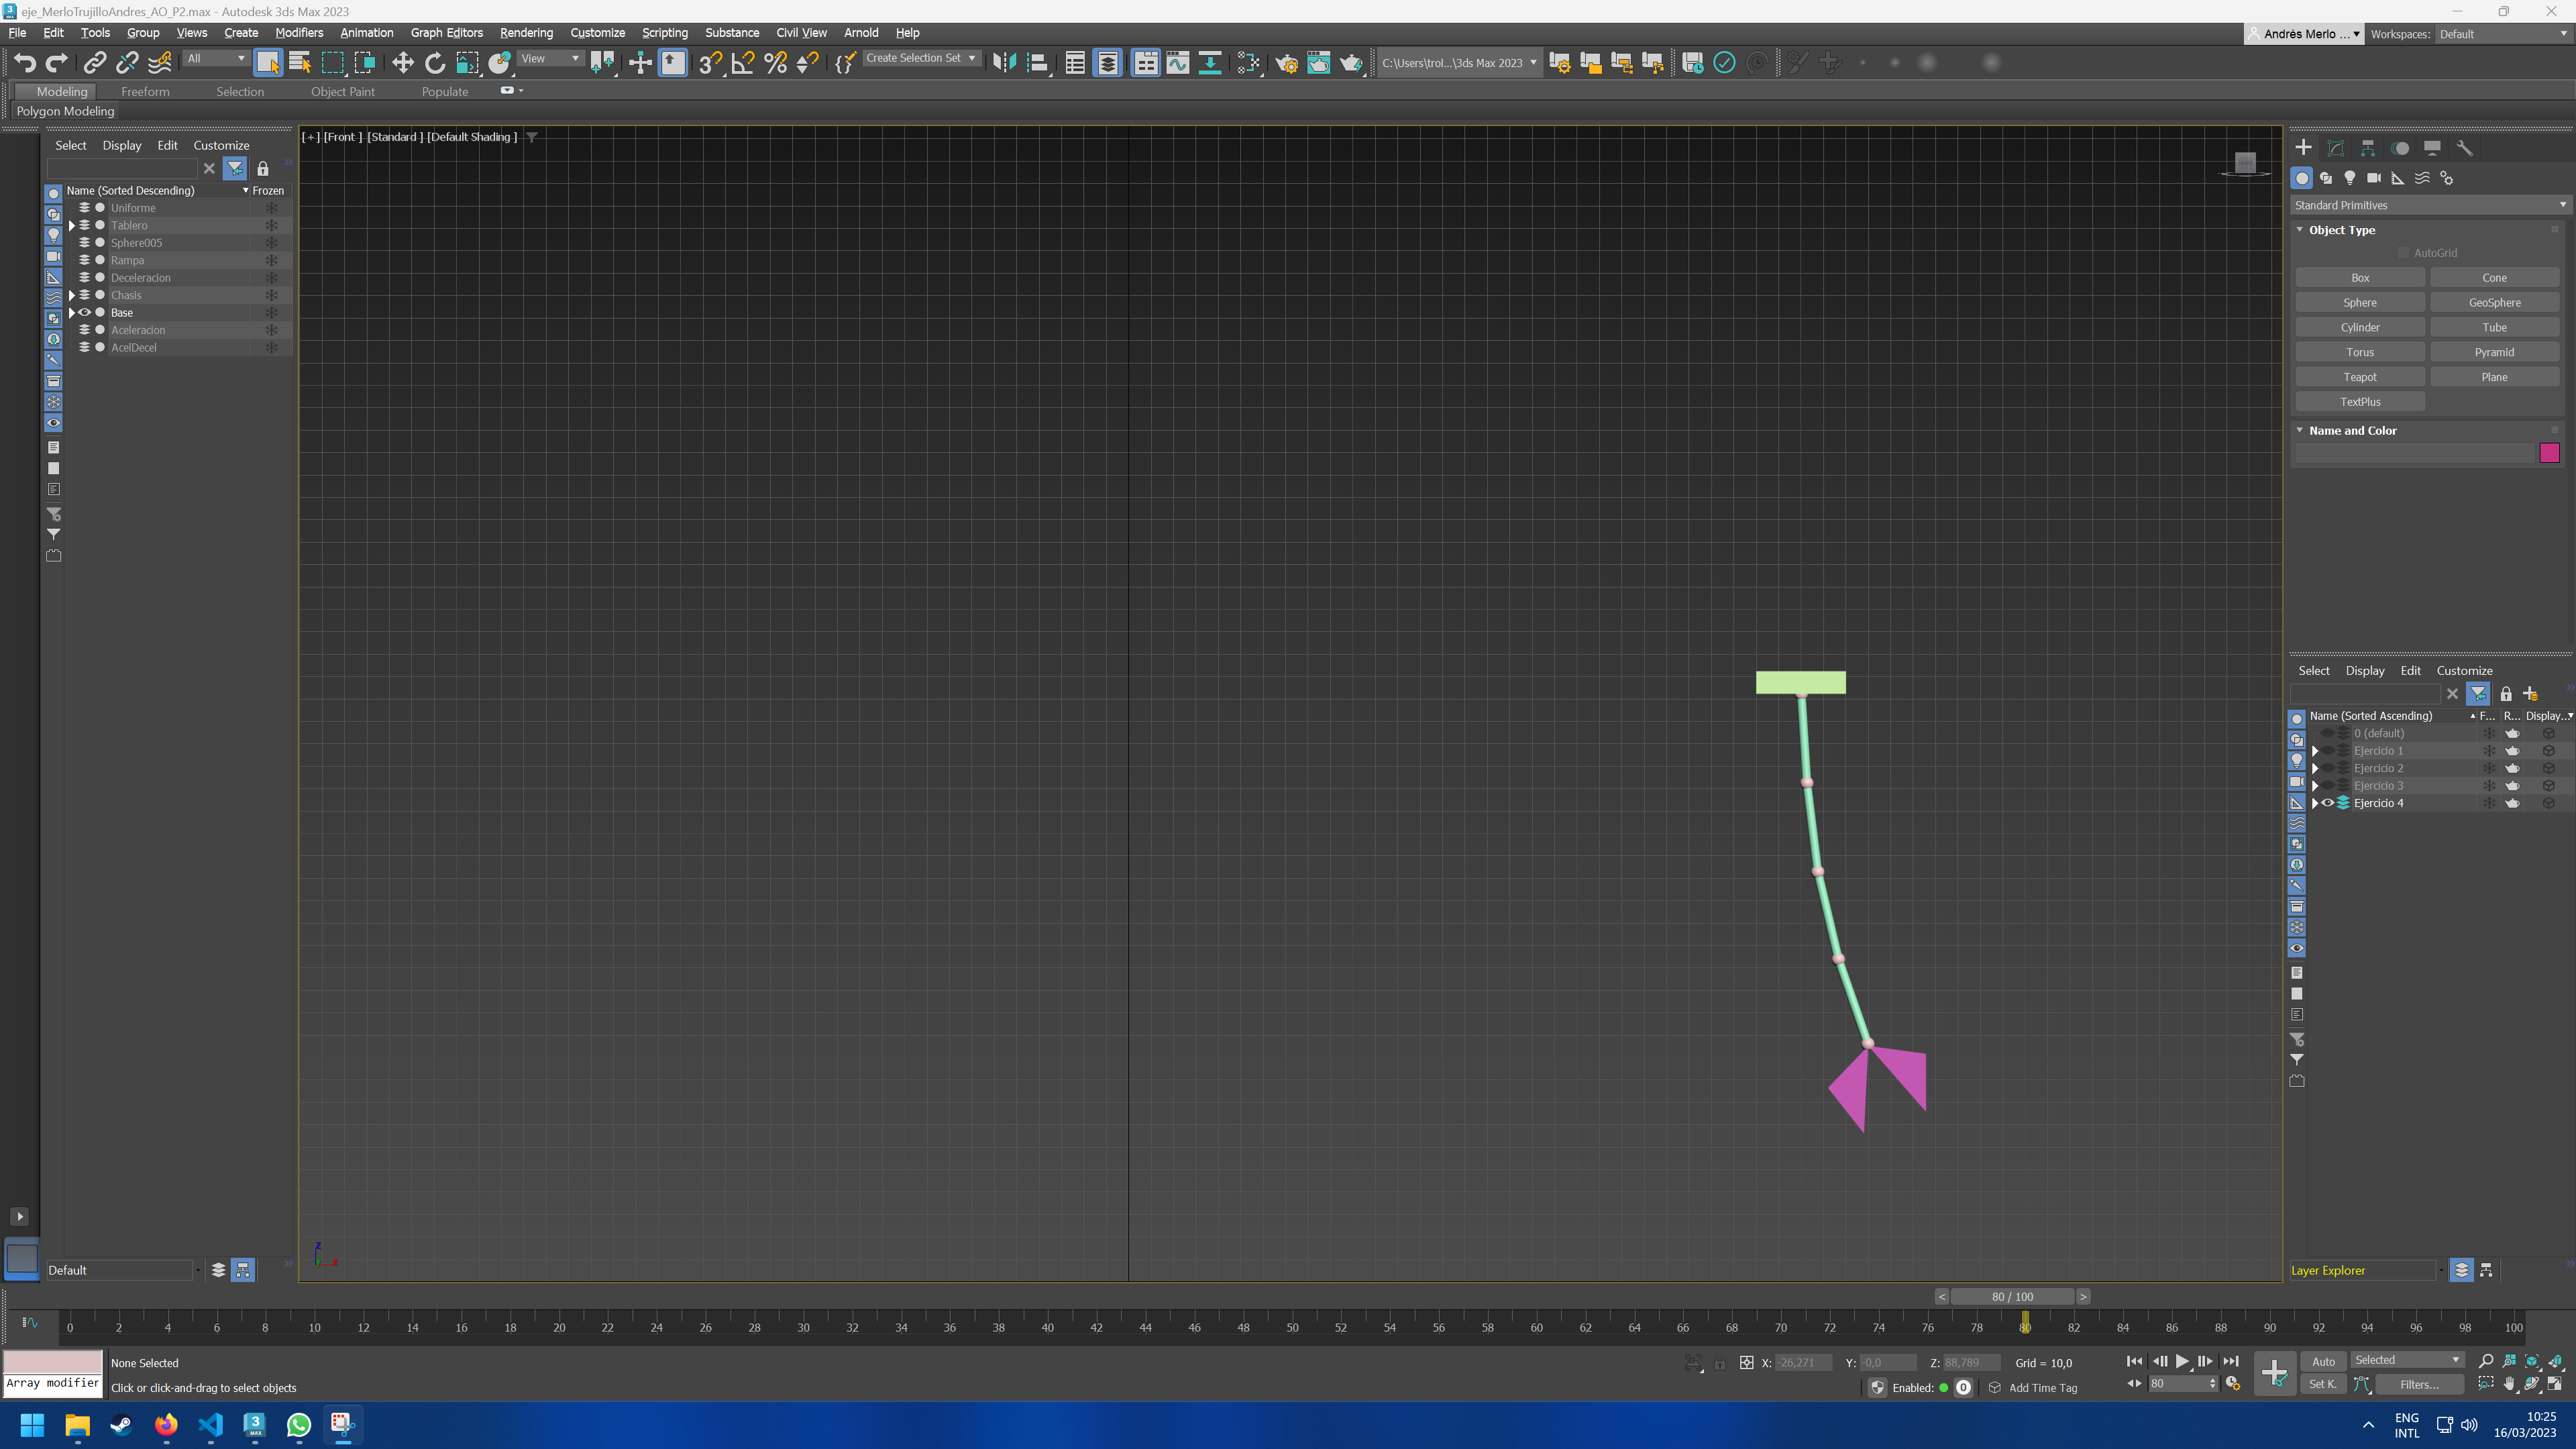
\includegraphics[width=\textwidth]{imagenes/Ejercicio4/keyframes/80.png}
        \caption{Rotación de los segmentos de la cadena en el instante 80.}
    \end{subfigure}
\end{figure}

\begin{figure}[H]\ContinuedFloat
    \centering
\begin{subfigure}[H]{0.48\textwidth}
    \centering
    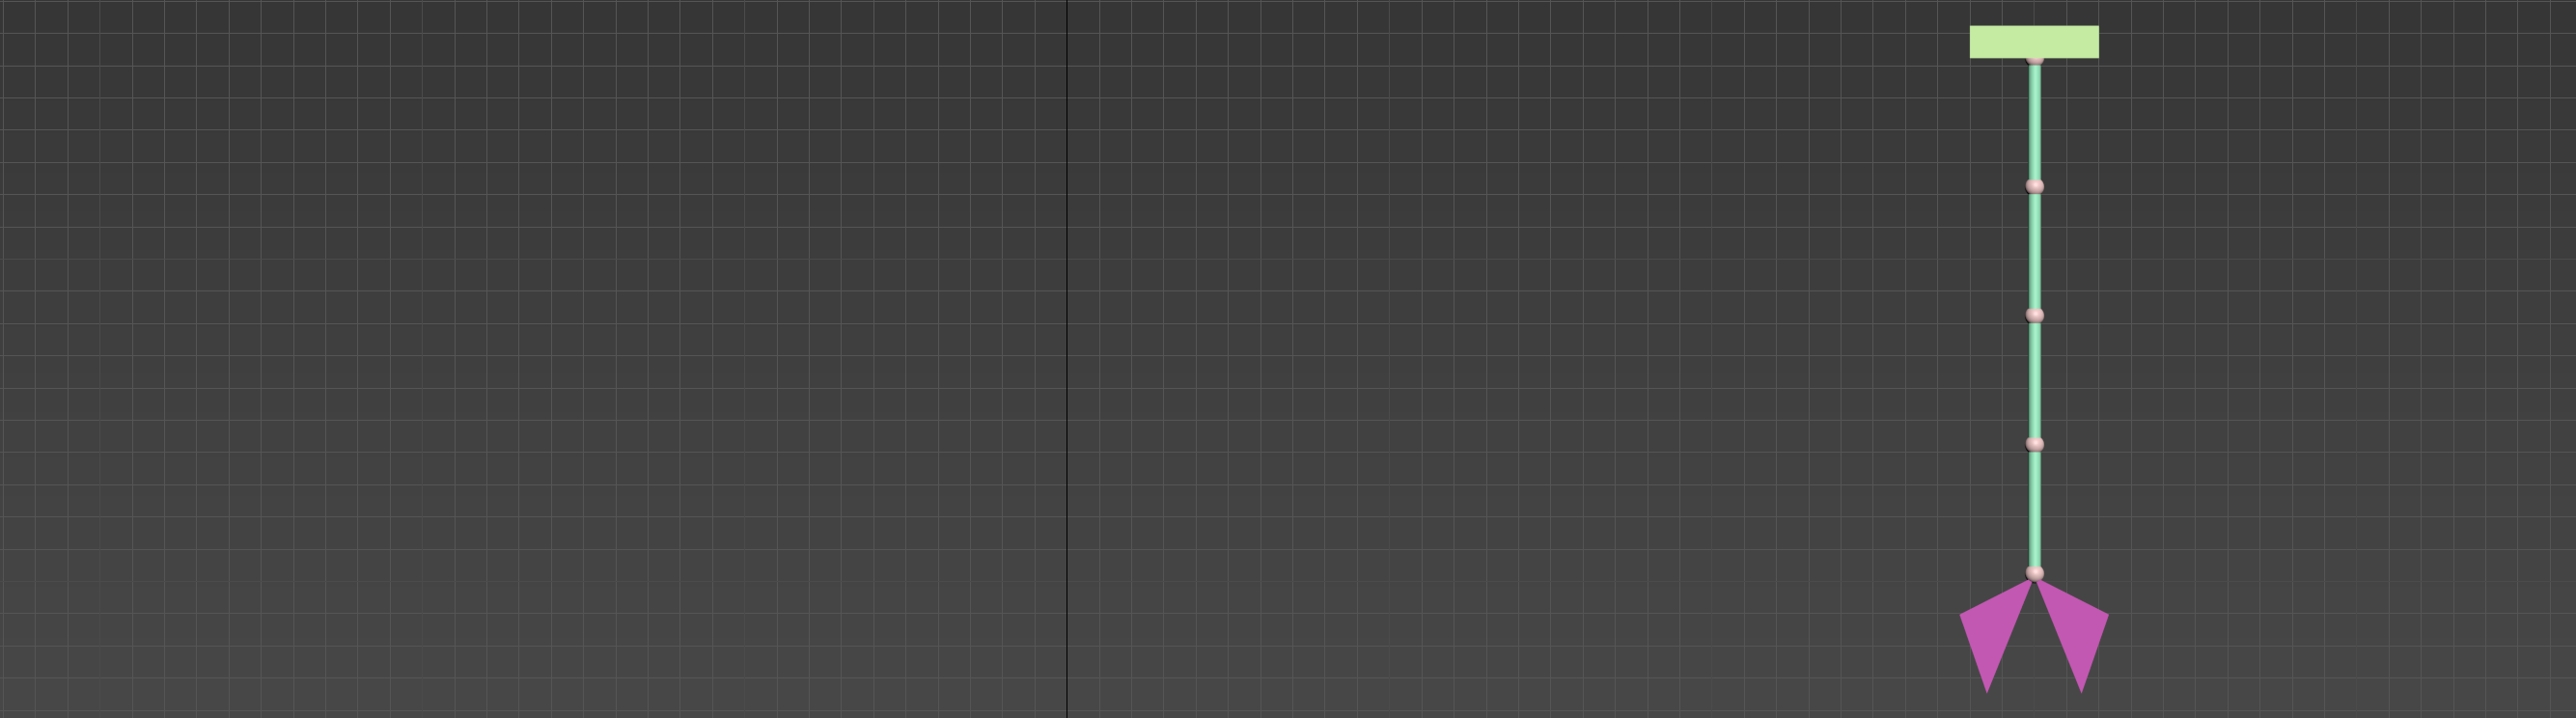
\includegraphics[width=\textwidth]{imagenes/Ejercicio4/keyframes/96.png}
    \caption{Rotación de los segmentos de la cadena en el instante 96.}
\end{subfigure}
\caption{\textit{Keyframes} de la plataforma y el brazo.}
\end{figure}

Se ha colocado el \textit{keyframe} en el instante 18, ya que sin él la animación de la rotación de la cadena debido a la velocidad no se completaría hasta que la plataforma se detuviera en el instante 30, lo que haría que la animación no fuera muy convincente. Al hacer esto, se ha logrado que la cadena rote completamente antes de que la plataforma se detenga.

\newpage
%curva
La curva para la animación de la plataforma es la siguiente:

%foto de la curva
\begin{figure}[H]
    \centering
    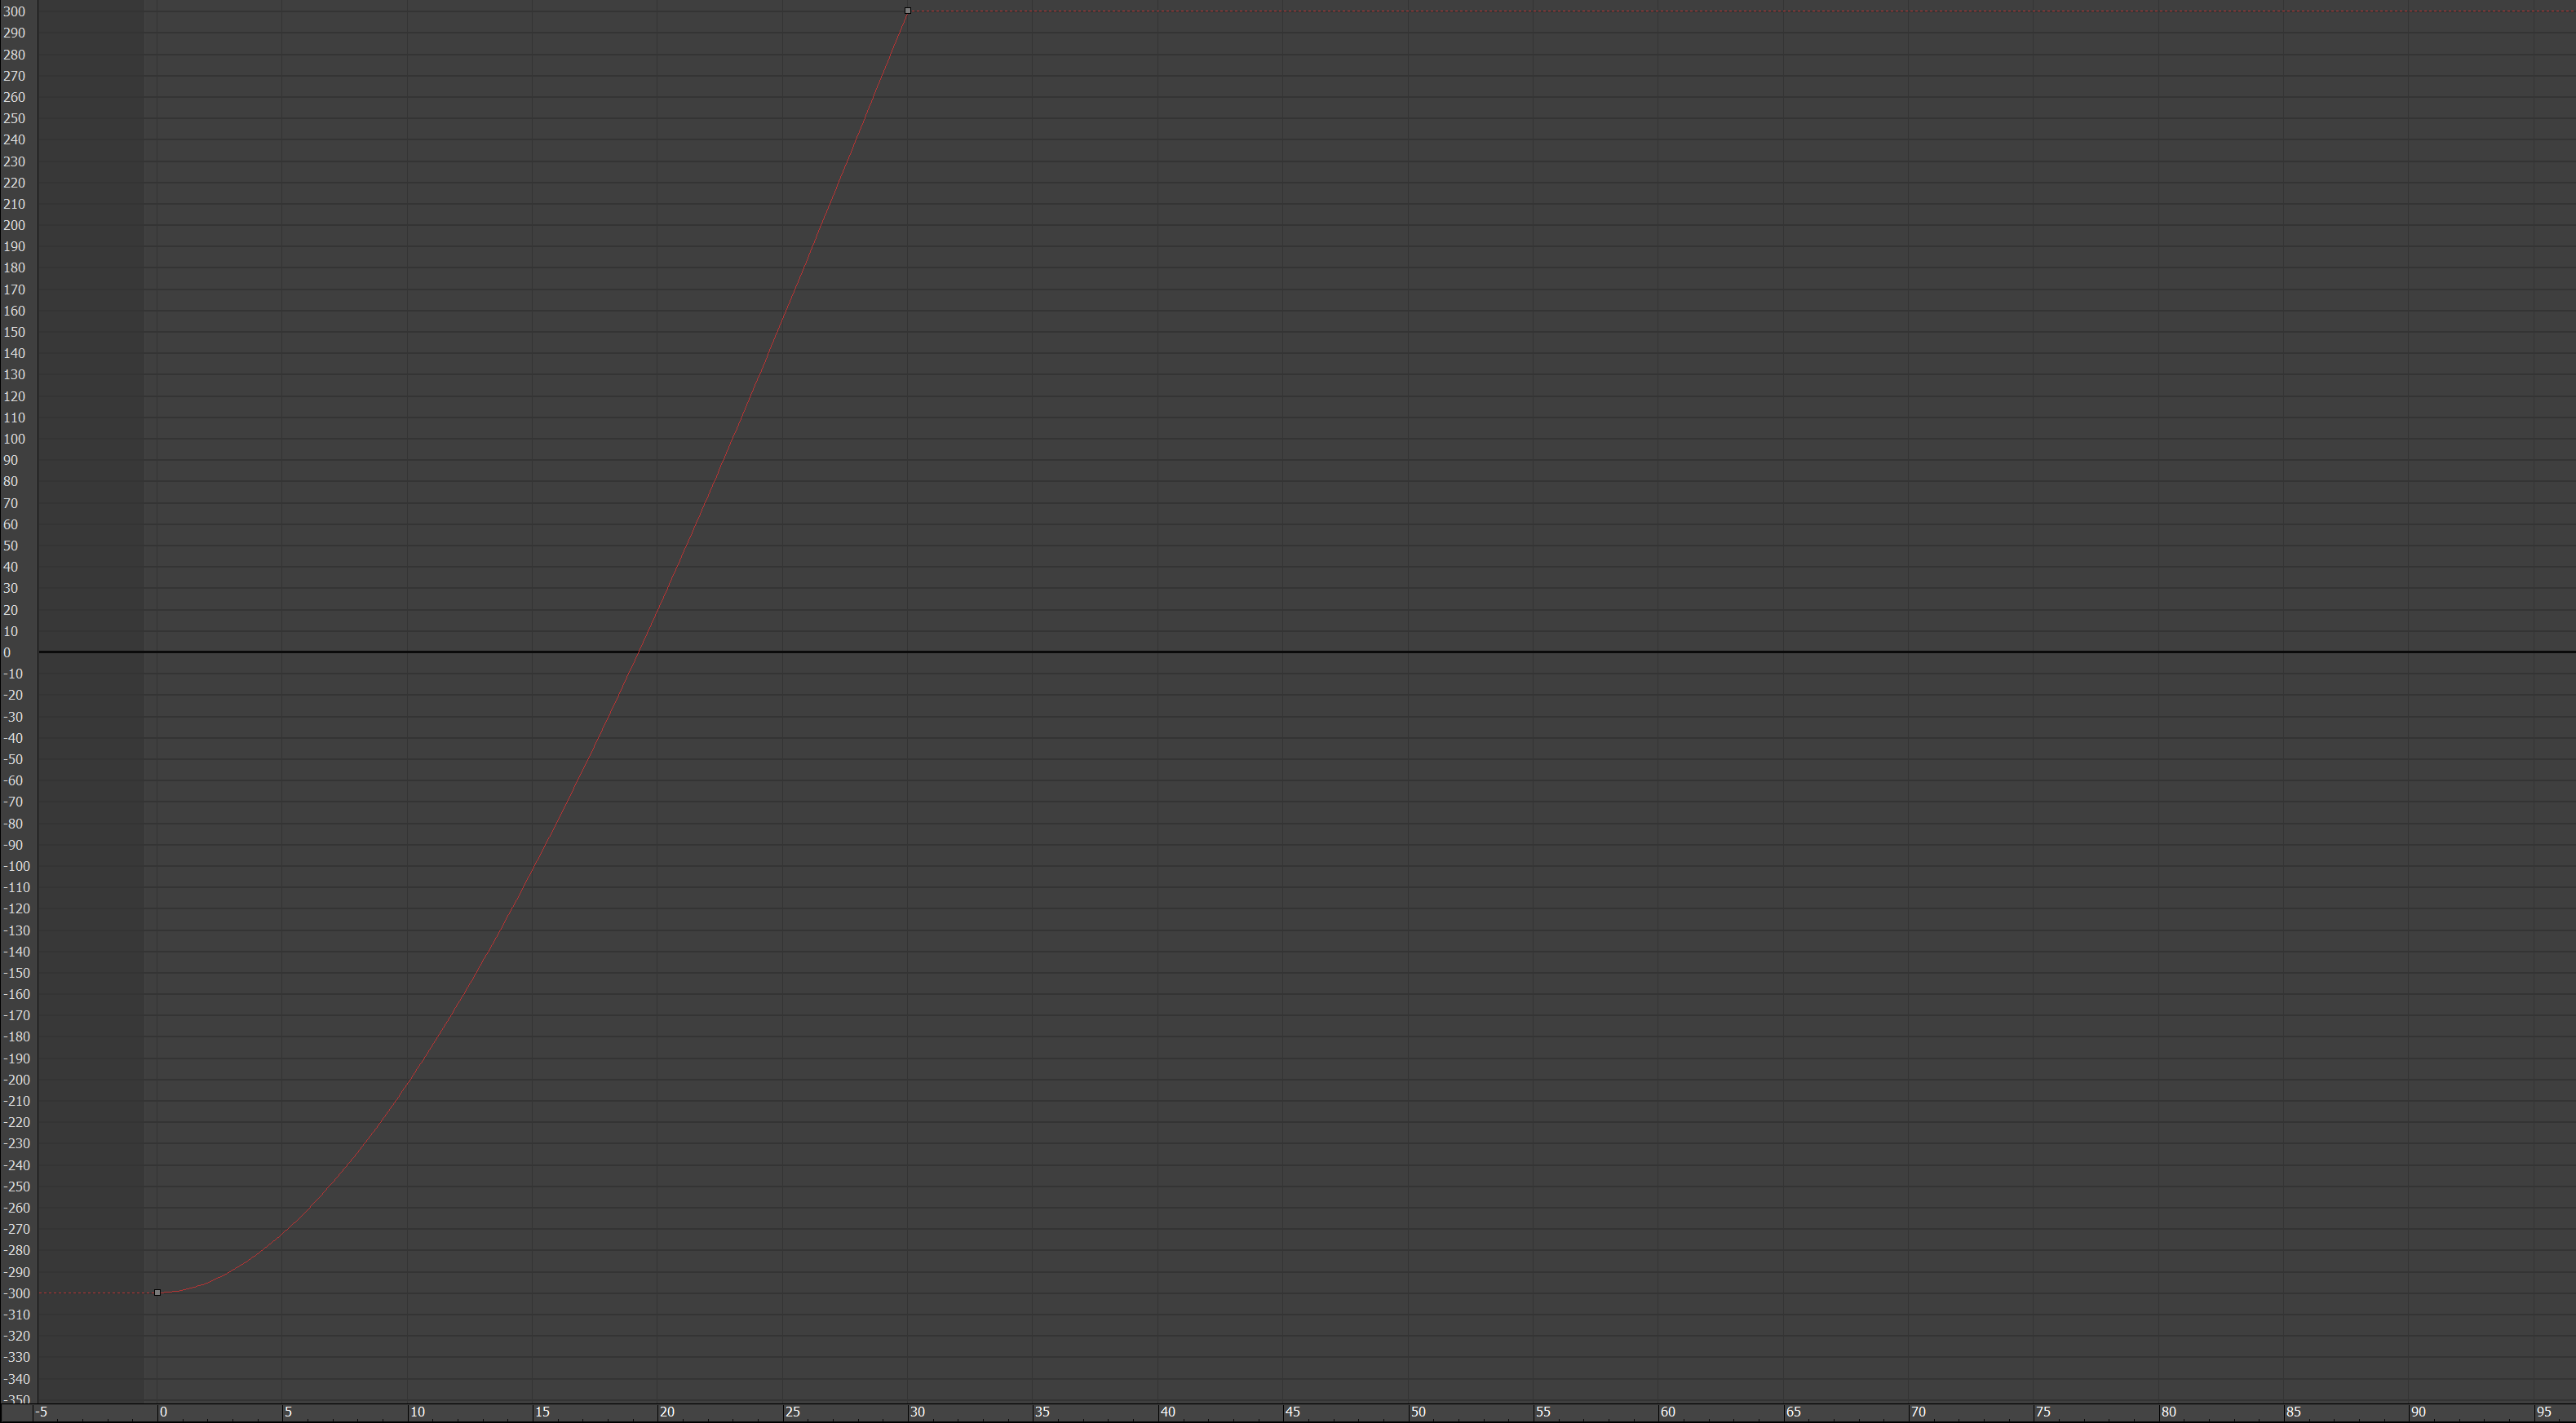
\includegraphics[width=0.8\textwidth]{imagenes/Ejercicio4/curvas/base/red.png}
    \caption{Curva de la posición en el eje X de la plataforma con respecto al tiempo.}
\end{figure}

Esta curva hace que la plataforma acelere al principio y se detenga bruscamente al llegar al punto final (mediante una cura lineal). Se ha realizado de esta manera para lograr que el latigazo que realiza la cadena parezca más realista.

% \newpage
\bigskip

Las curvas de los segmentos de la cadena son muy similares entre sí, por lo que solo voy a mostrar uno.

%foto de la curva
\begin{figure}[H]
    \centering
    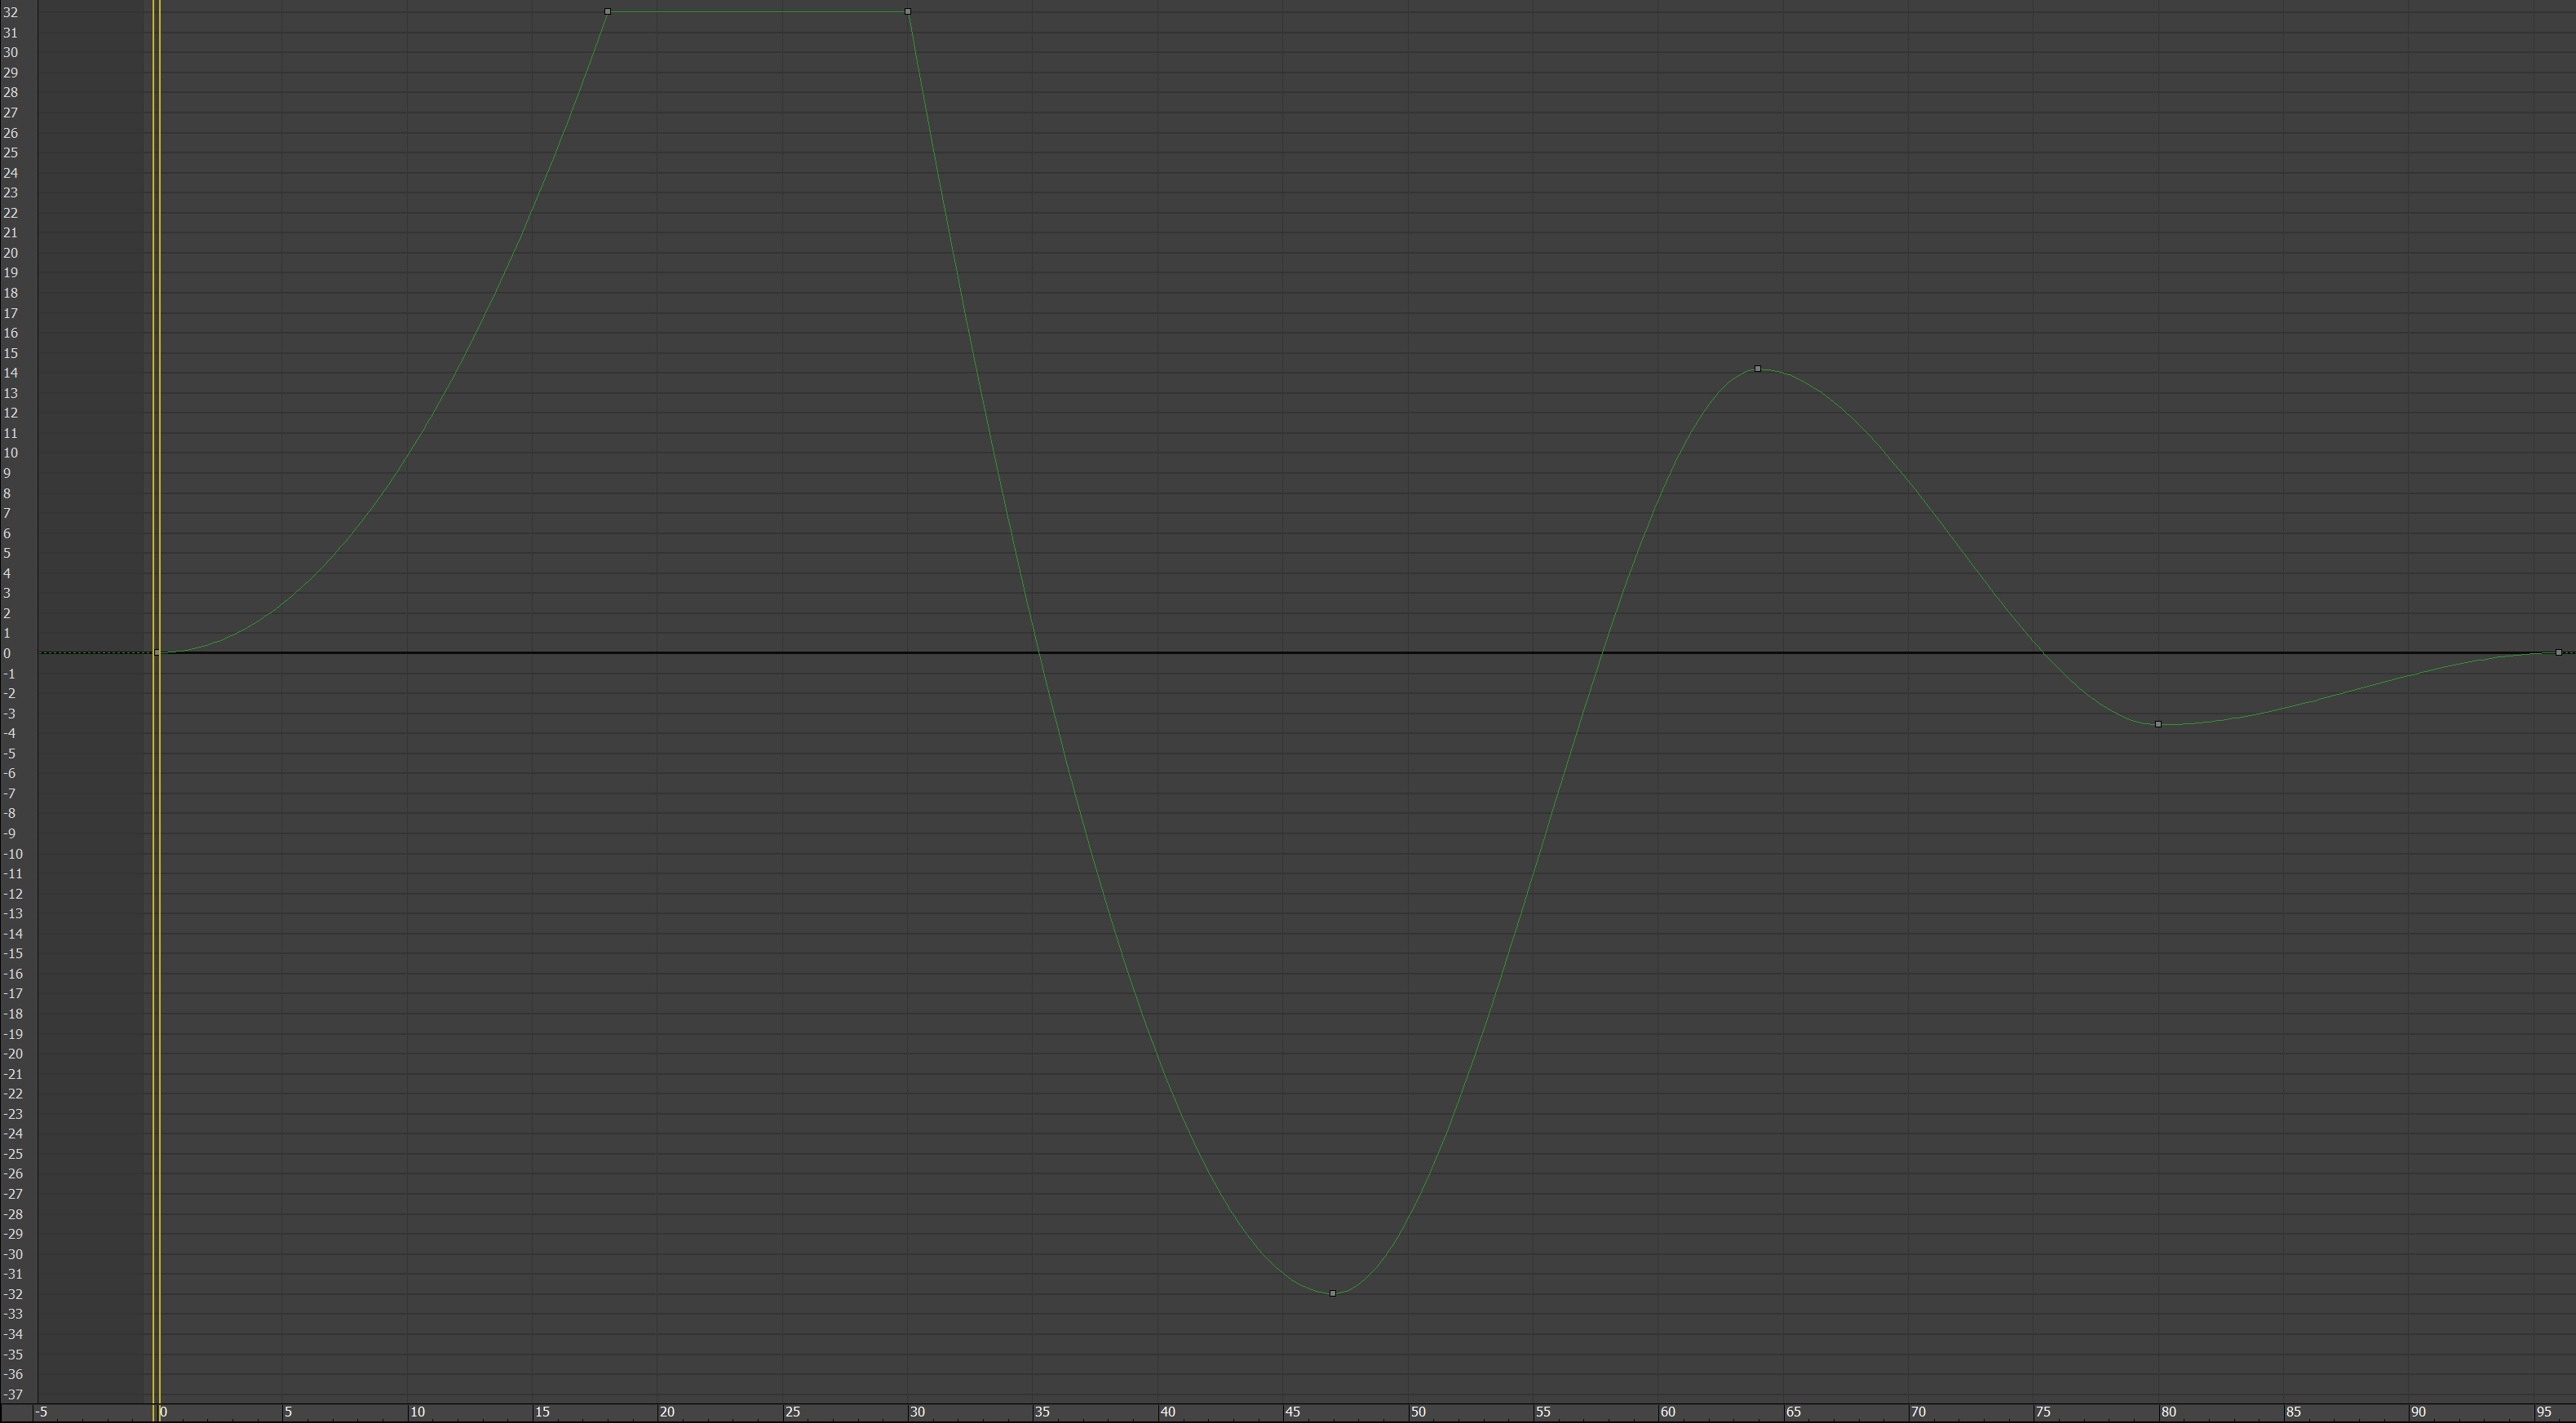
\includegraphics[width=0.8\textwidth]{imagenes/Ejercicio4/curvas/segmentos/green.png}
    \caption{Curva para la rotación en el eje Y de los segmentos con respecto el tiempo.}
\end{figure}

Esta curva sigue la misma aceleración que la plataforma al principio de la animación, logrando que el movimiento sea más natural. A partir del instante 18, la curva se mantiene constante al no requerir rotación. Cuando la plataforma se detiene, se utiliza una curva lineal, ya que la energía que tenía la plataforma se transfiere a la cadena y finalmente se utilizan curvas de aceleración, desaceleración y \textit{Slow in/Slow out} (combinación de ambas) para simular el vaivén que realiza la cadena antes de detenerse debido a las distintas fuerzas.


\end{document}
